\documentclass[10pt]{article}
\usepackage[utf8]{inputenc}
\usepackage[T1]{fontenc}
\usepackage{amsmath}
\usepackage{amsfonts}
\usepackage{amssymb}
\usepackage[version=4]{mhchem}
\usepackage{stmaryrd}
\usepackage{graphicx}
\usepackage[export]{adjustbox}
\graphicspath{ {./images/} }
\usepackage{bbold}
\usepackage{mathrsfs}

\title{Bias-Variance Decomposition }

\author{}
\date{}


\def\Perp{\perp\!\!\!\perp}

\begin{document}
\maketitle
Machine Learning Course - CS-433

Oct 11, 2023

Nicolas Flammarion

EPFL

\section*{Last time}
How can we judge if a given predictor is good?

How to select the best models of a family?

$\rightarrow$ Bound the difference between the true and empirical risks

$\rightarrow$ Split data into train and test sets (learn with the train and test on the test)

Motivation: Hyperparameters search (which often control the complexity)

But we haven't investigated the role of the complexity of the class

\section*{Today}
How does the risk behave as a function of the complexity of the model class?

$\Rightarrow$ Bias-Variance tradeoff

It will help us to decide how complex and rich we should make our model

Before: quantitative

Now: qualitative

\section*{A small experiment: 1D-regression}
True function

\begin{center}
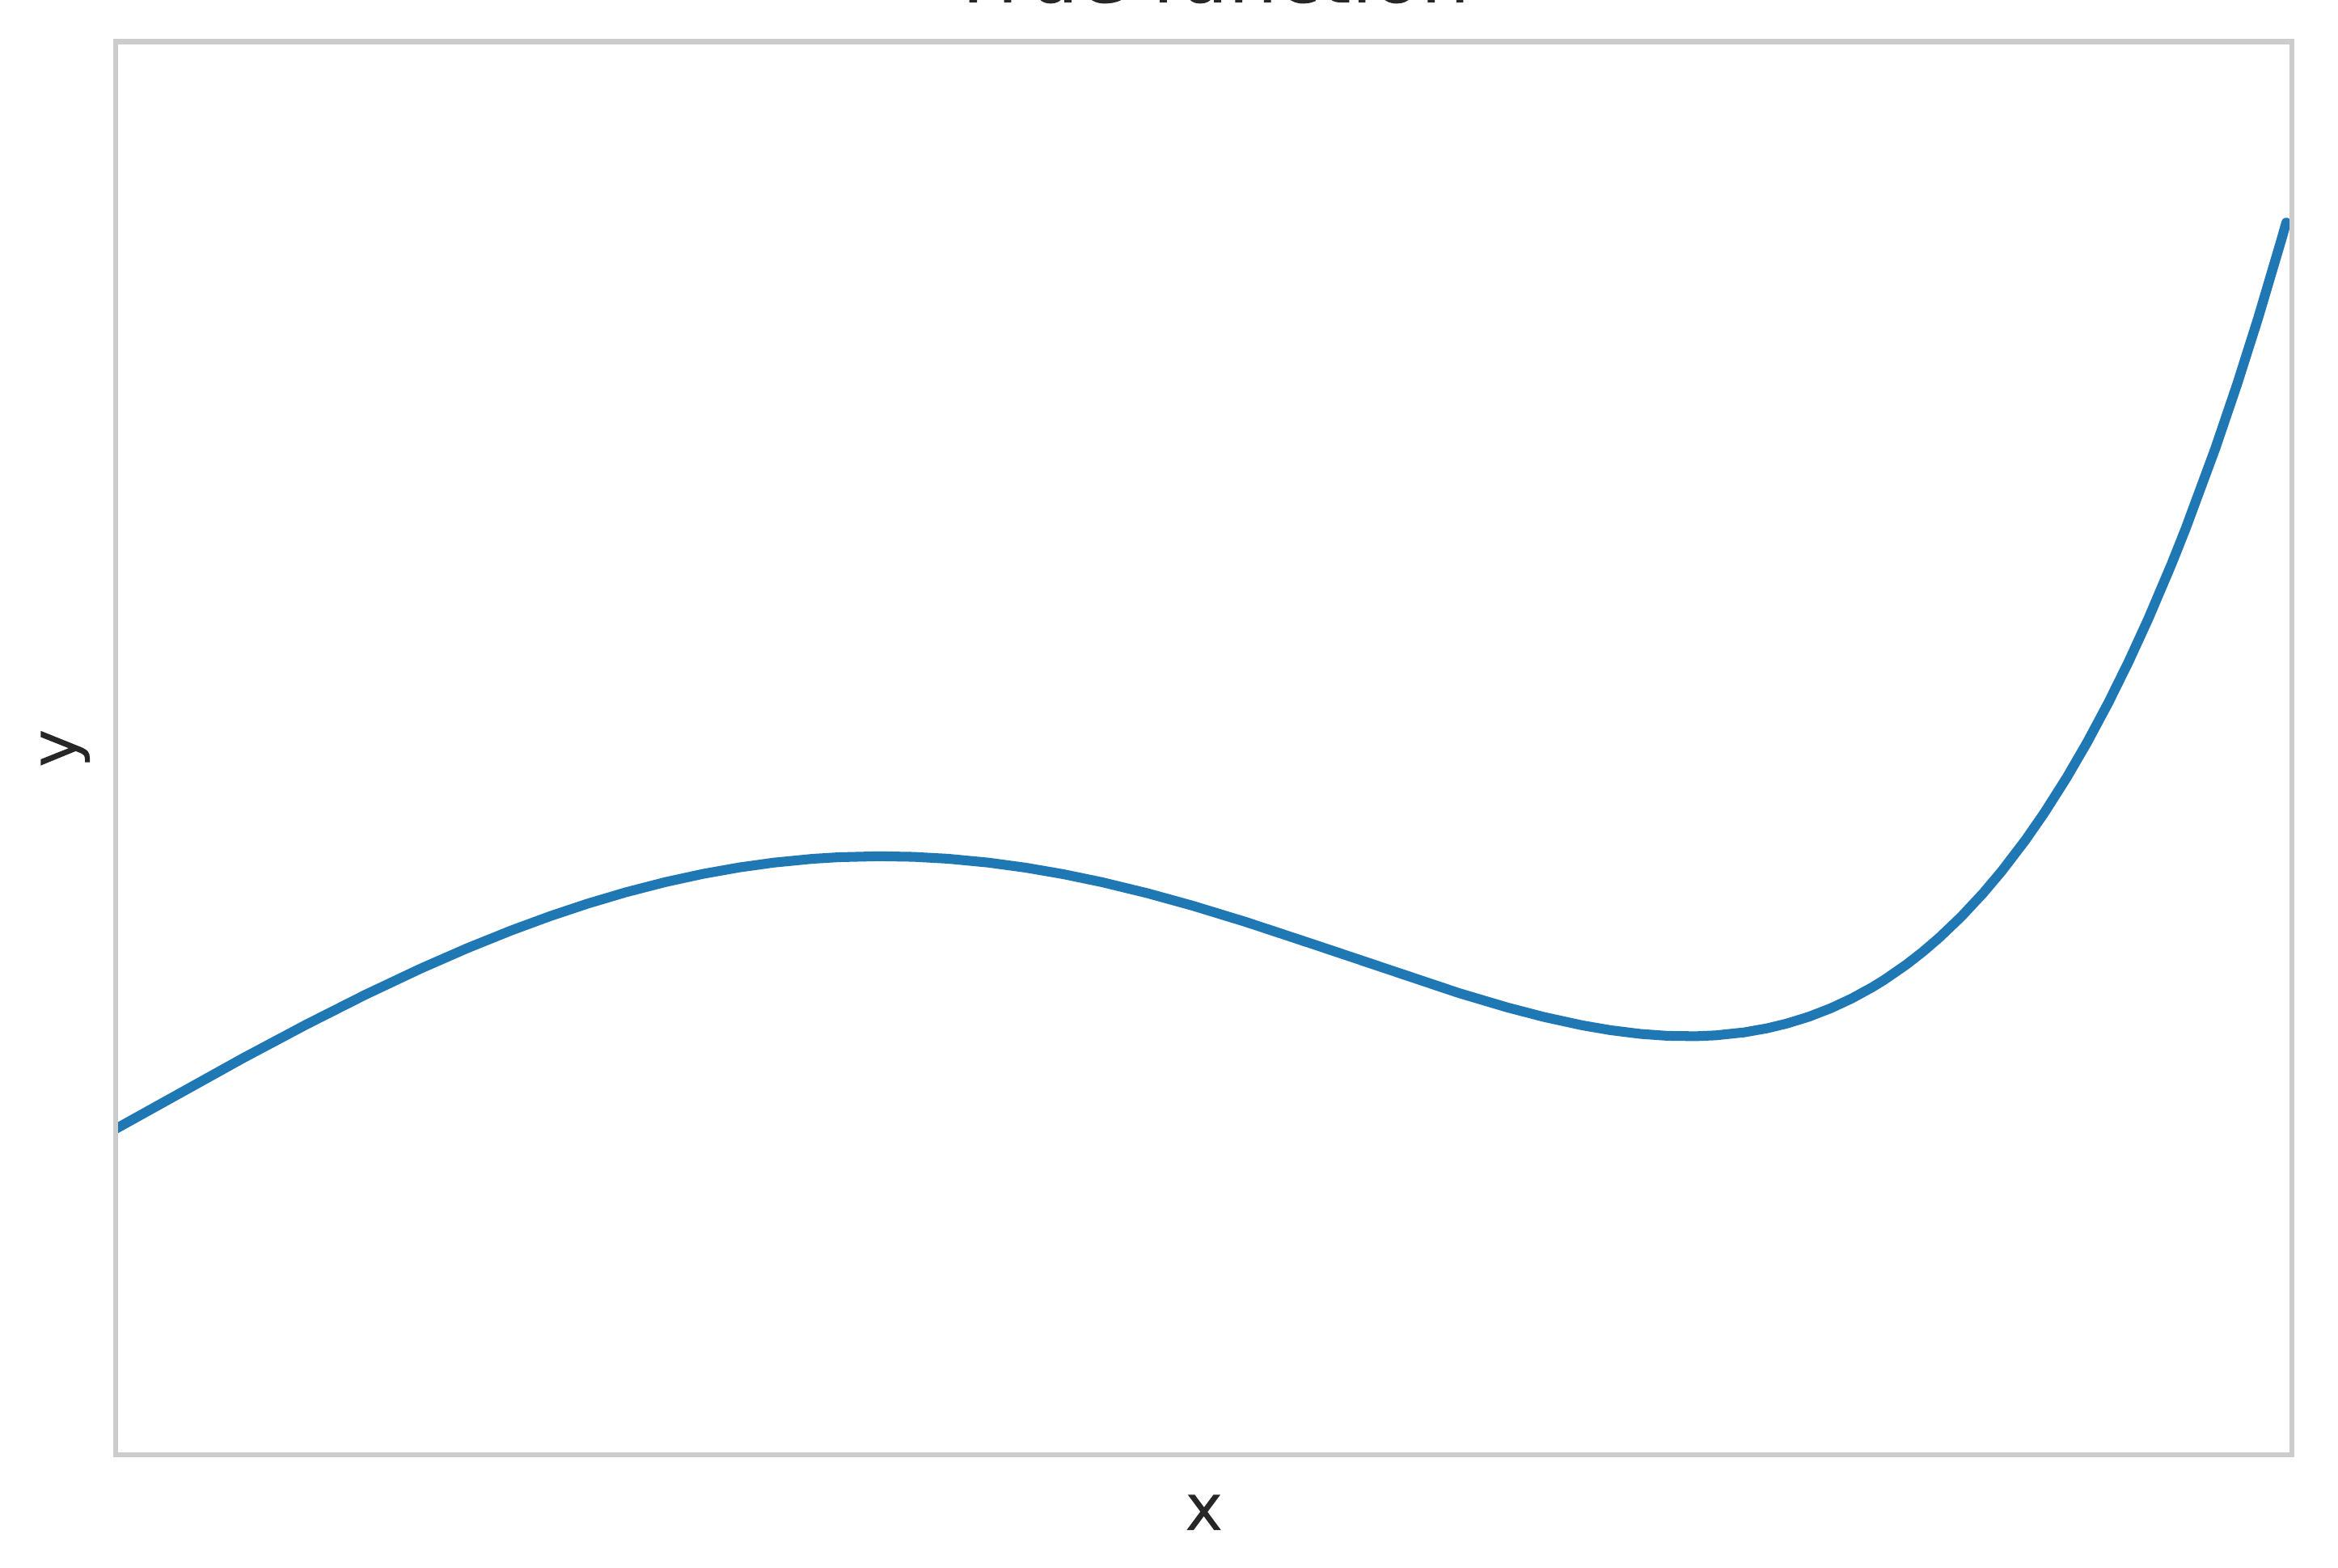
\includegraphics[max width=\textwidth]{2023_12_30_442f876157646883c2c9g-04}
\end{center}

\section*{A small experiment: 1D-regression}
Sampled training set

\begin{center}
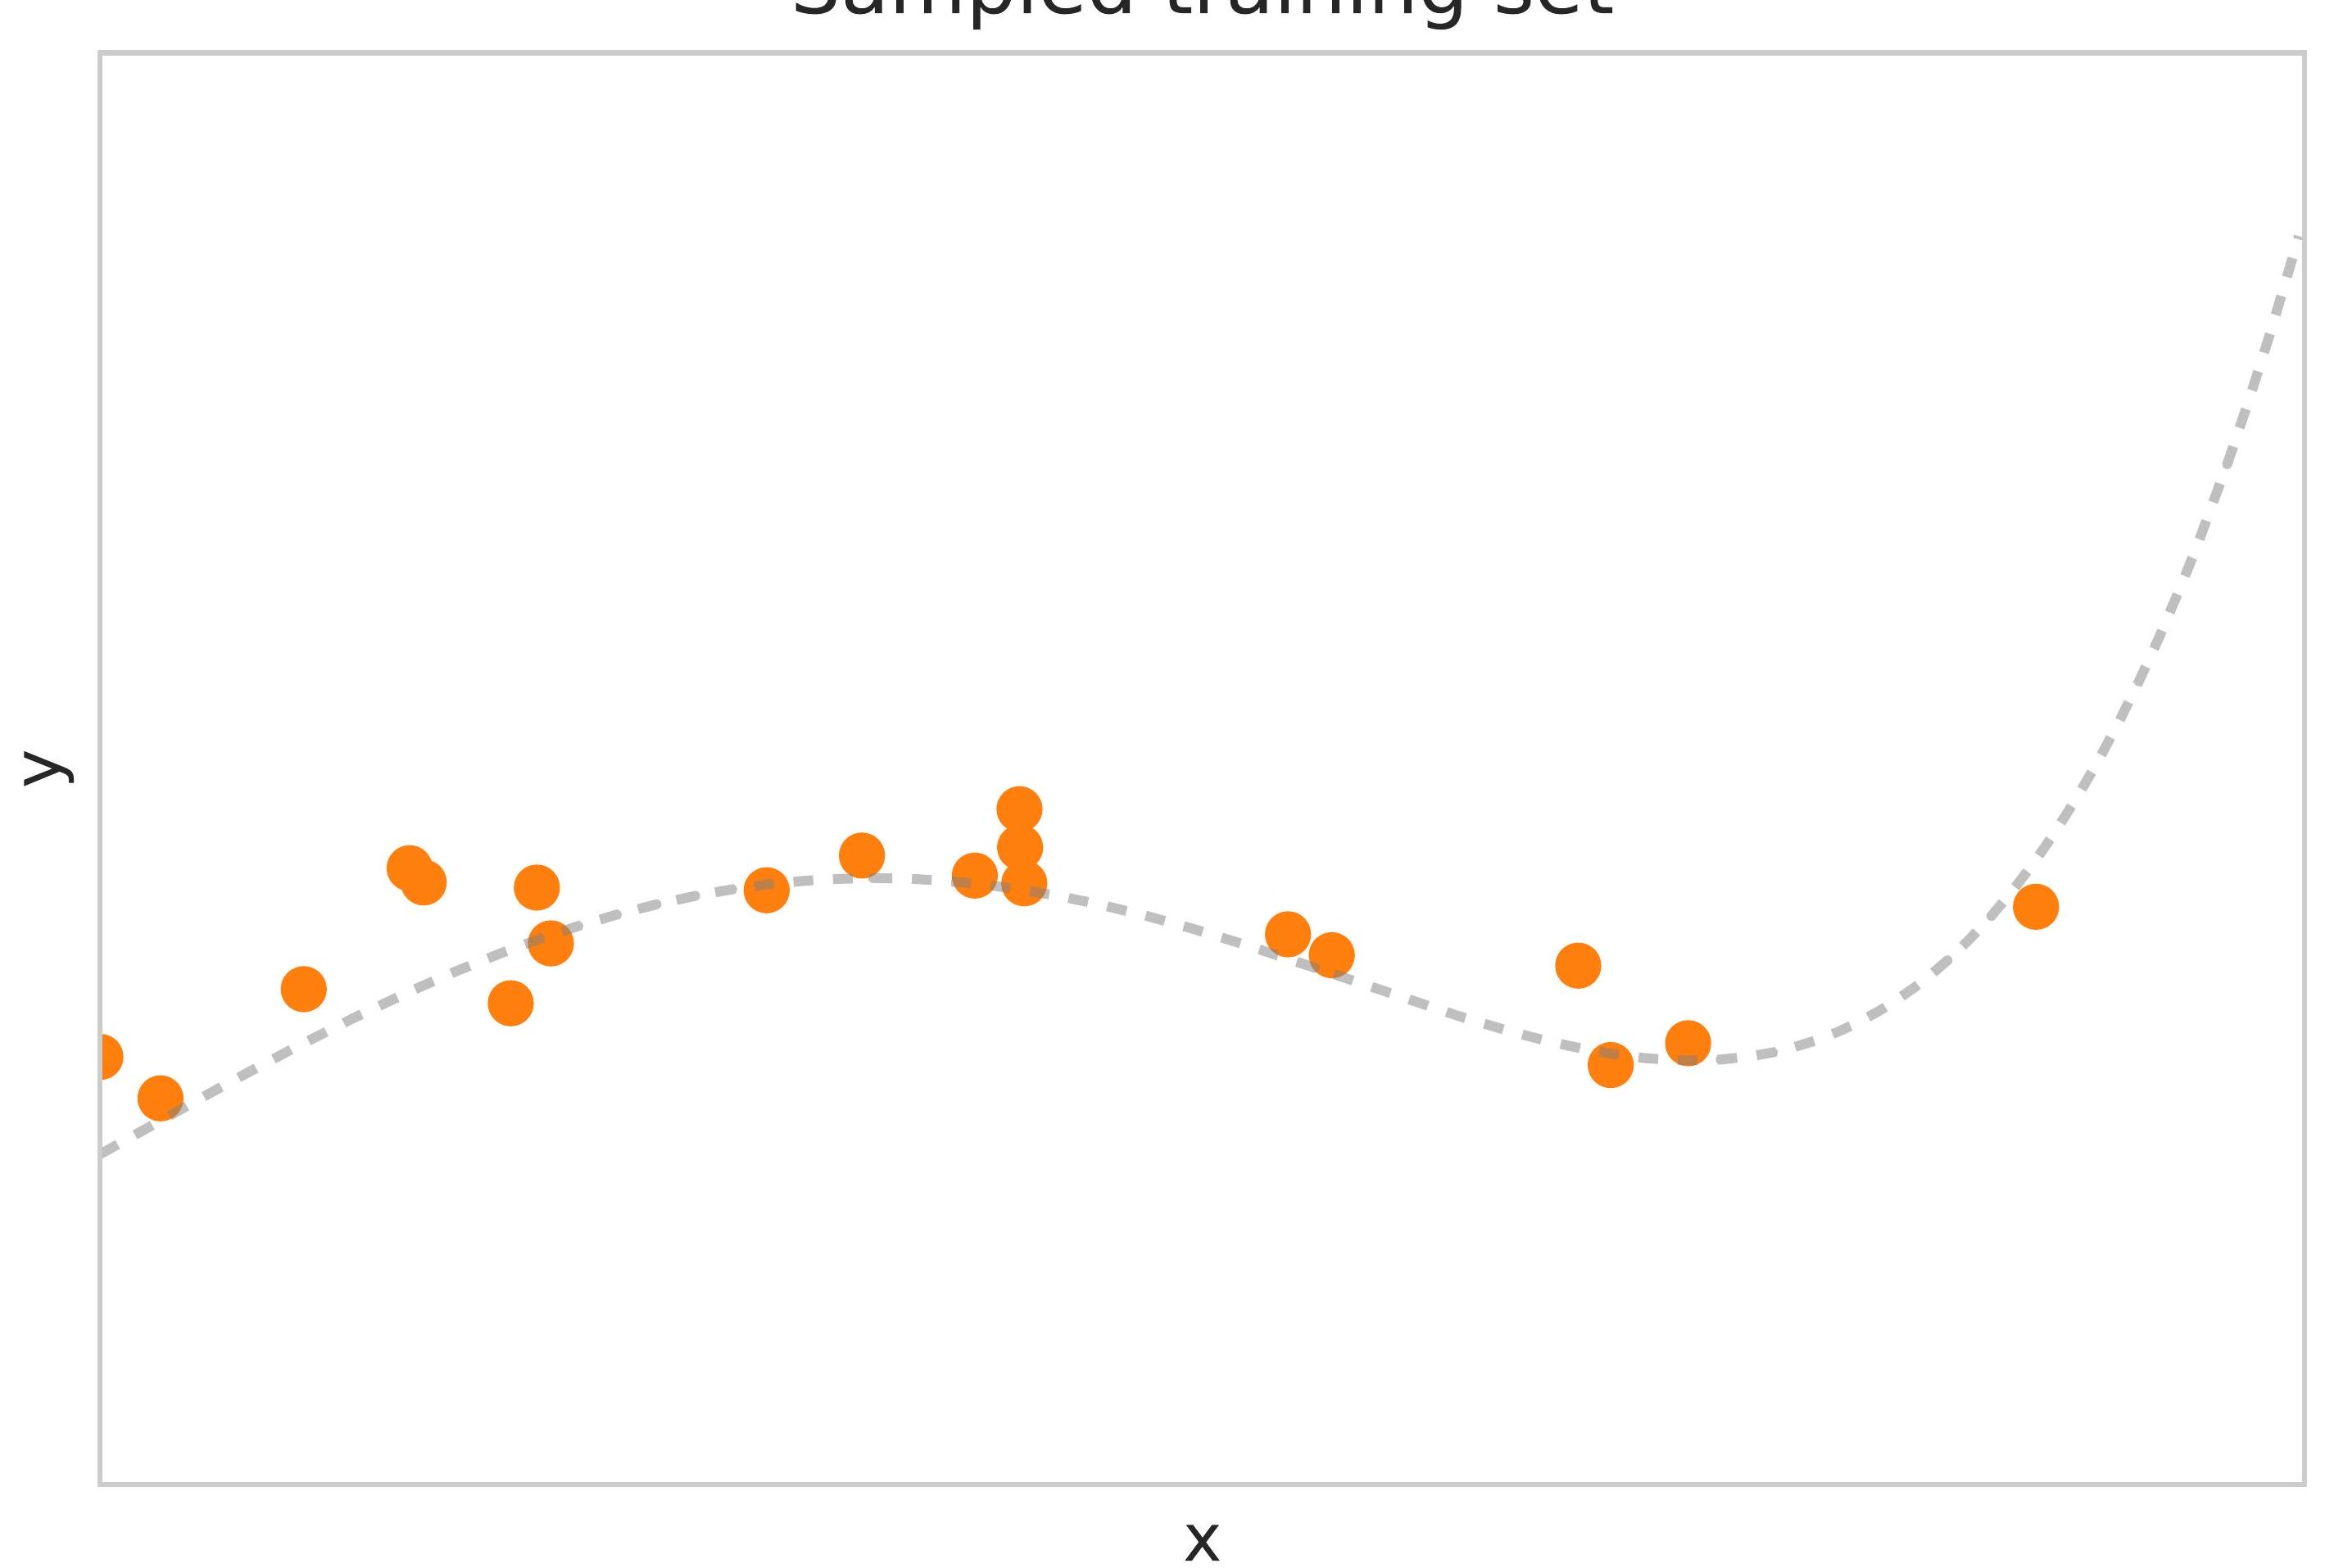
\includegraphics[max width=\textwidth]{2023_12_30_442f876157646883c2c9g-05}
\end{center}

Linear regression using polynomial feature expansion $\left(x, x^{2}, x^{3}, \cdots, x^{d}\right)$ The maximum degree $d$ measures the complexity of the class

$\Rightarrow$ How far should you go?

\section*{Simple model: bad fit}
Training fit (degree 1)

\begin{center}
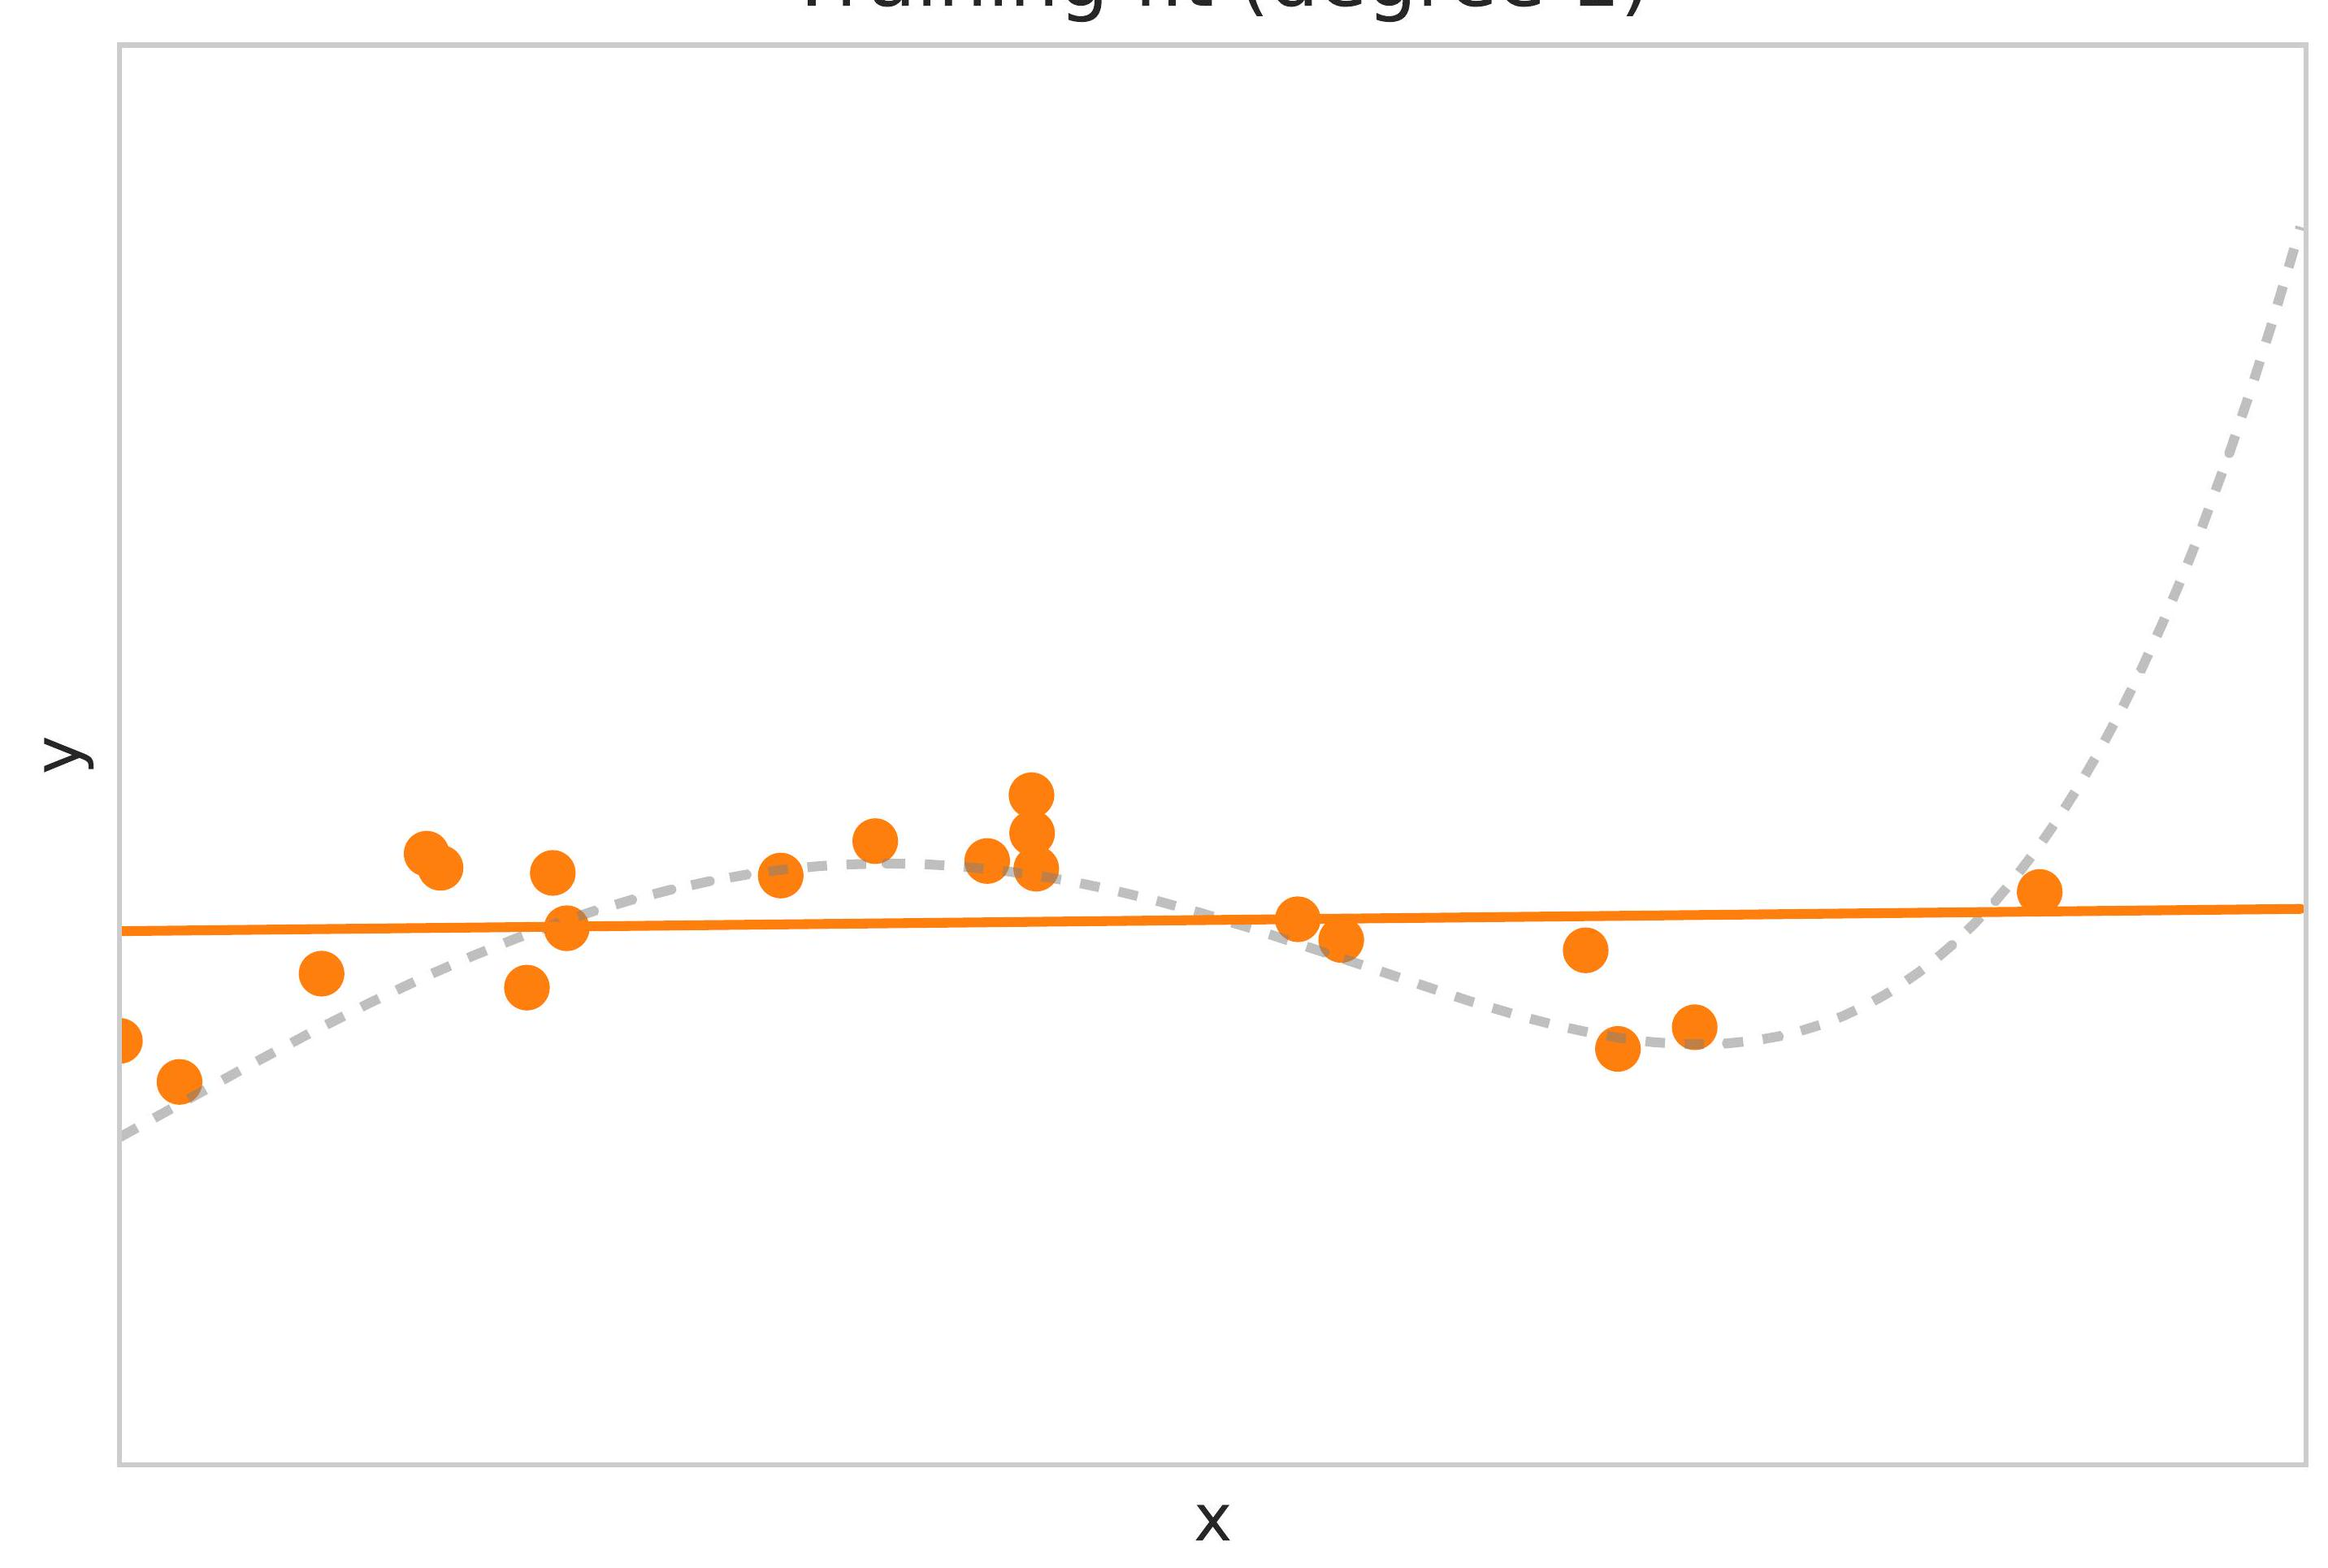
\includegraphics[max width=\textwidth]{2023_12_30_442f876157646883c2c9g-06}
\end{center}

No linear function would be a good predictor. The model class is not rich enough

\section*{Complex model: good fit?}
\begin{center}
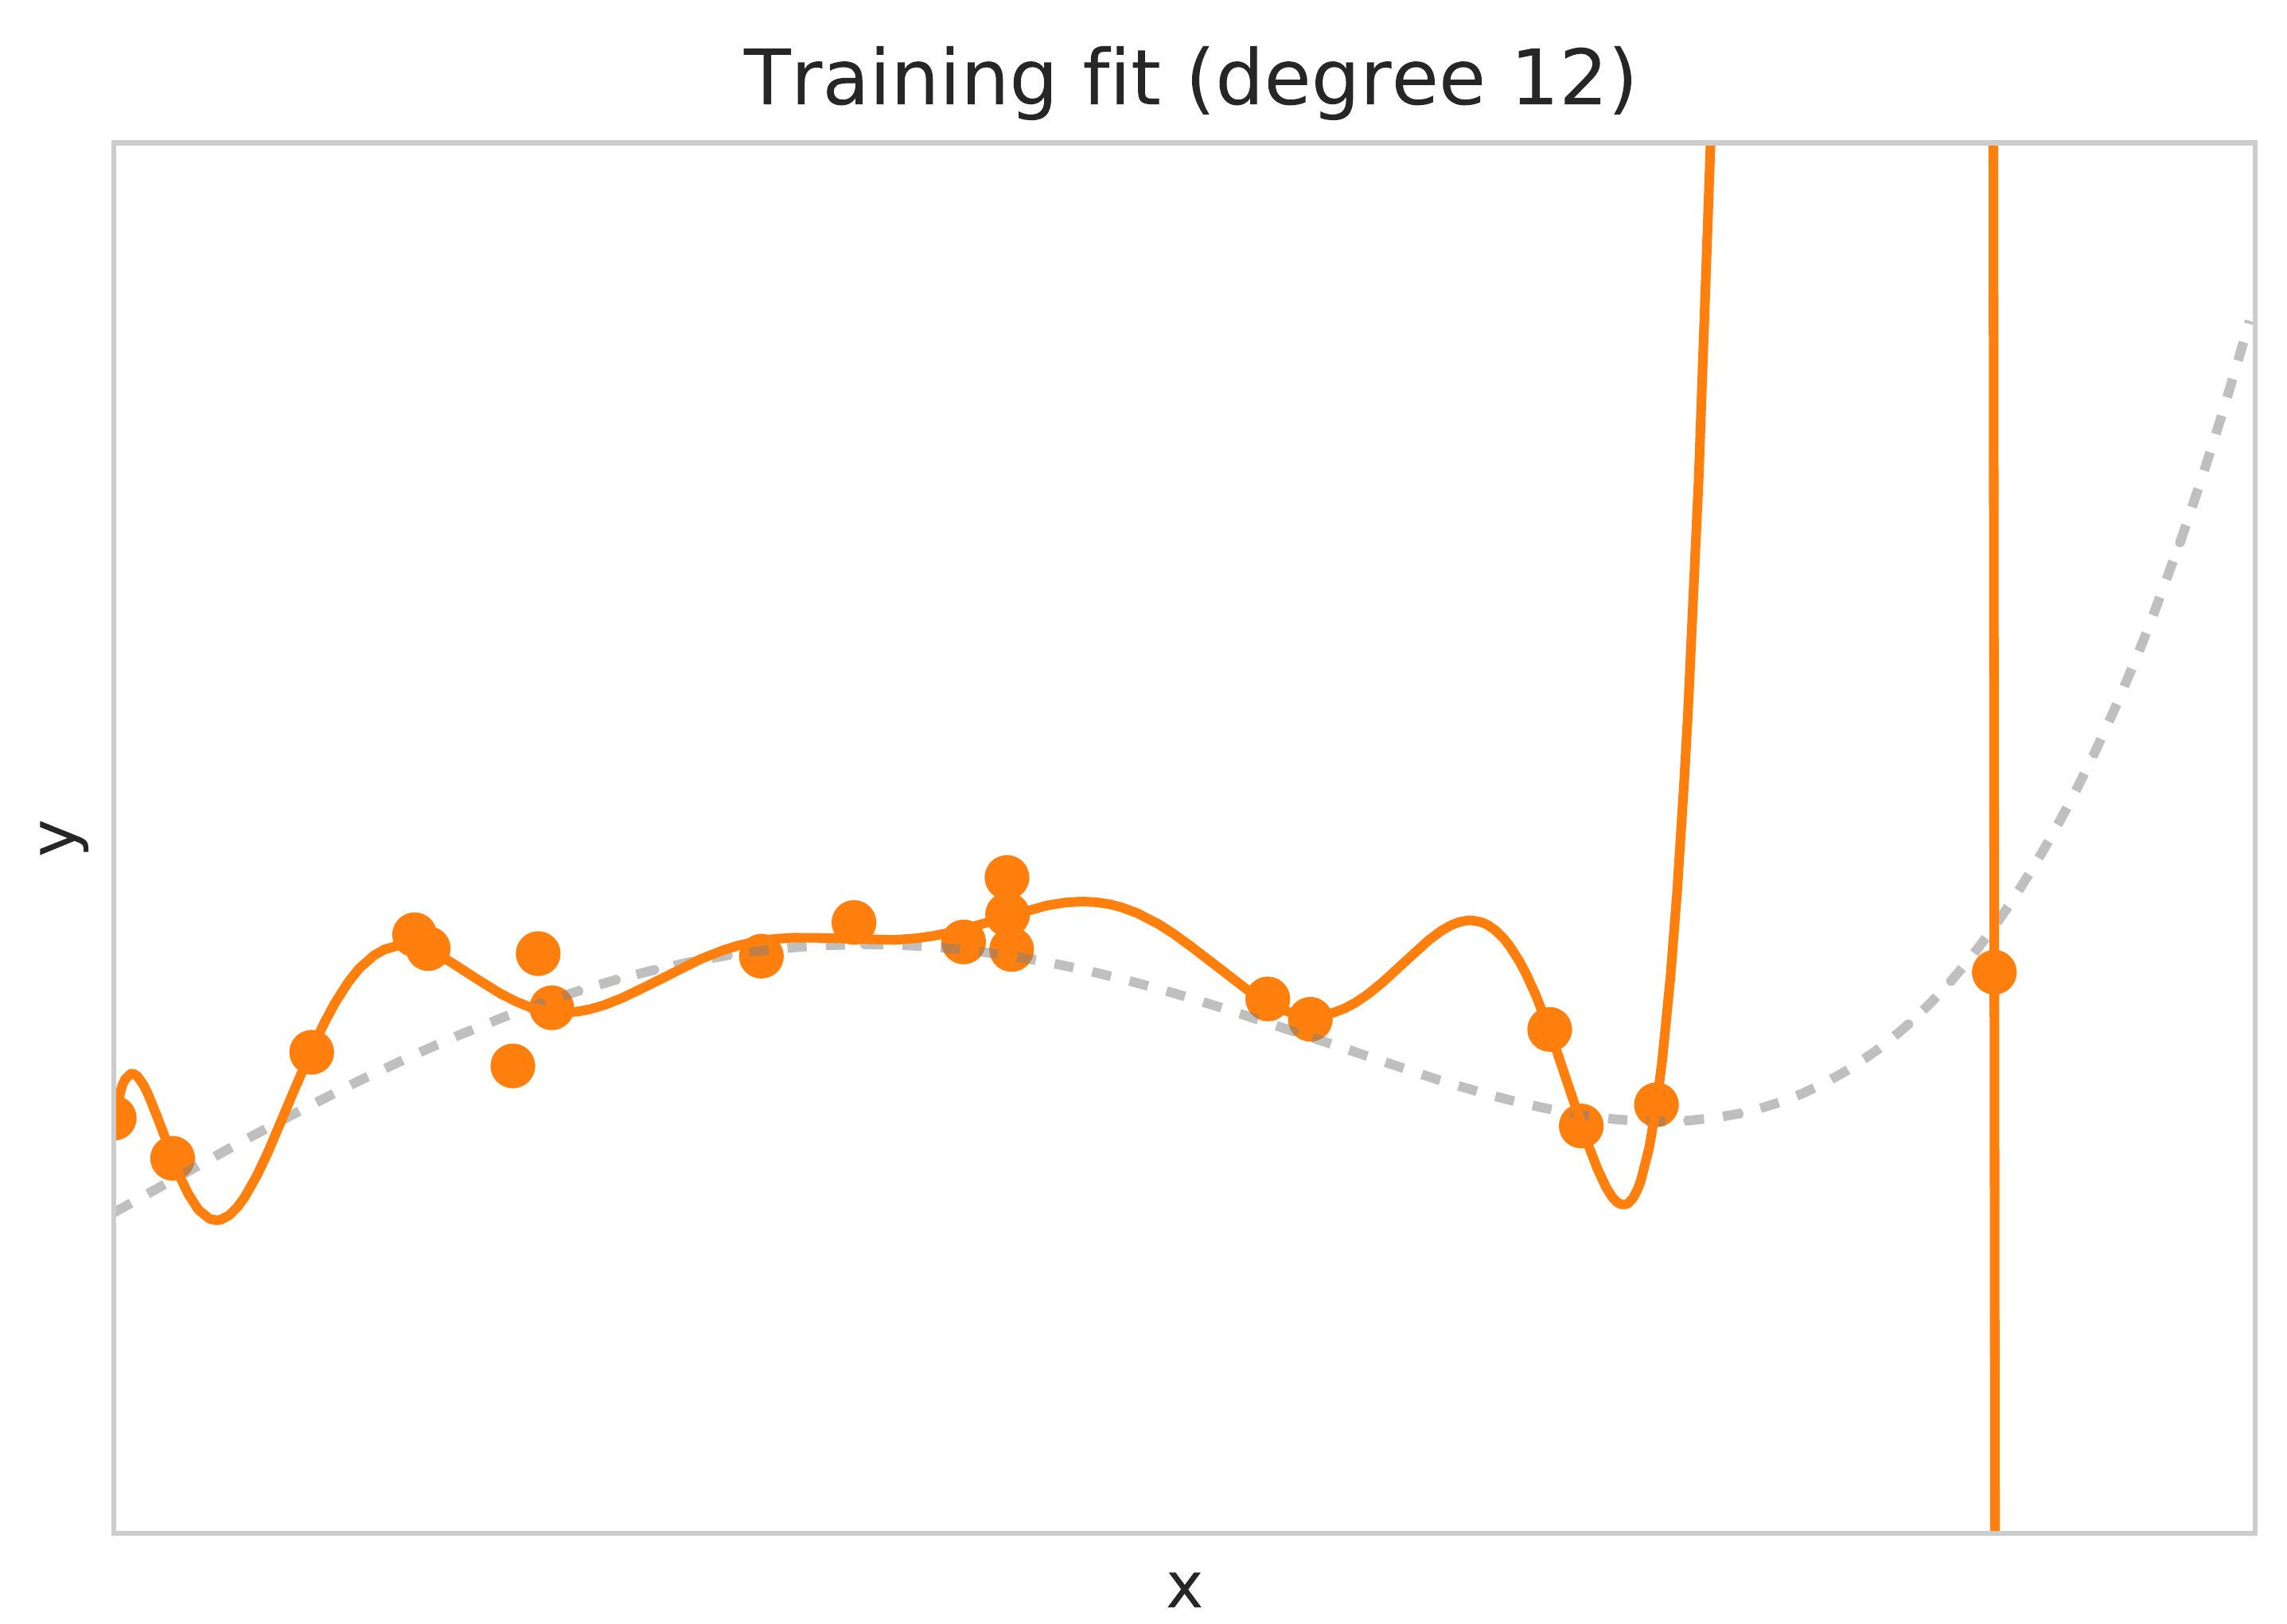
\includegraphics[max width=\textwidth]{2023_12_30_442f876157646883c2c9g-07}
\end{center}

High degree polynomial will be a good fit. But?

\section*{But there is randomness in the data}
Sampled training set

\begin{center}
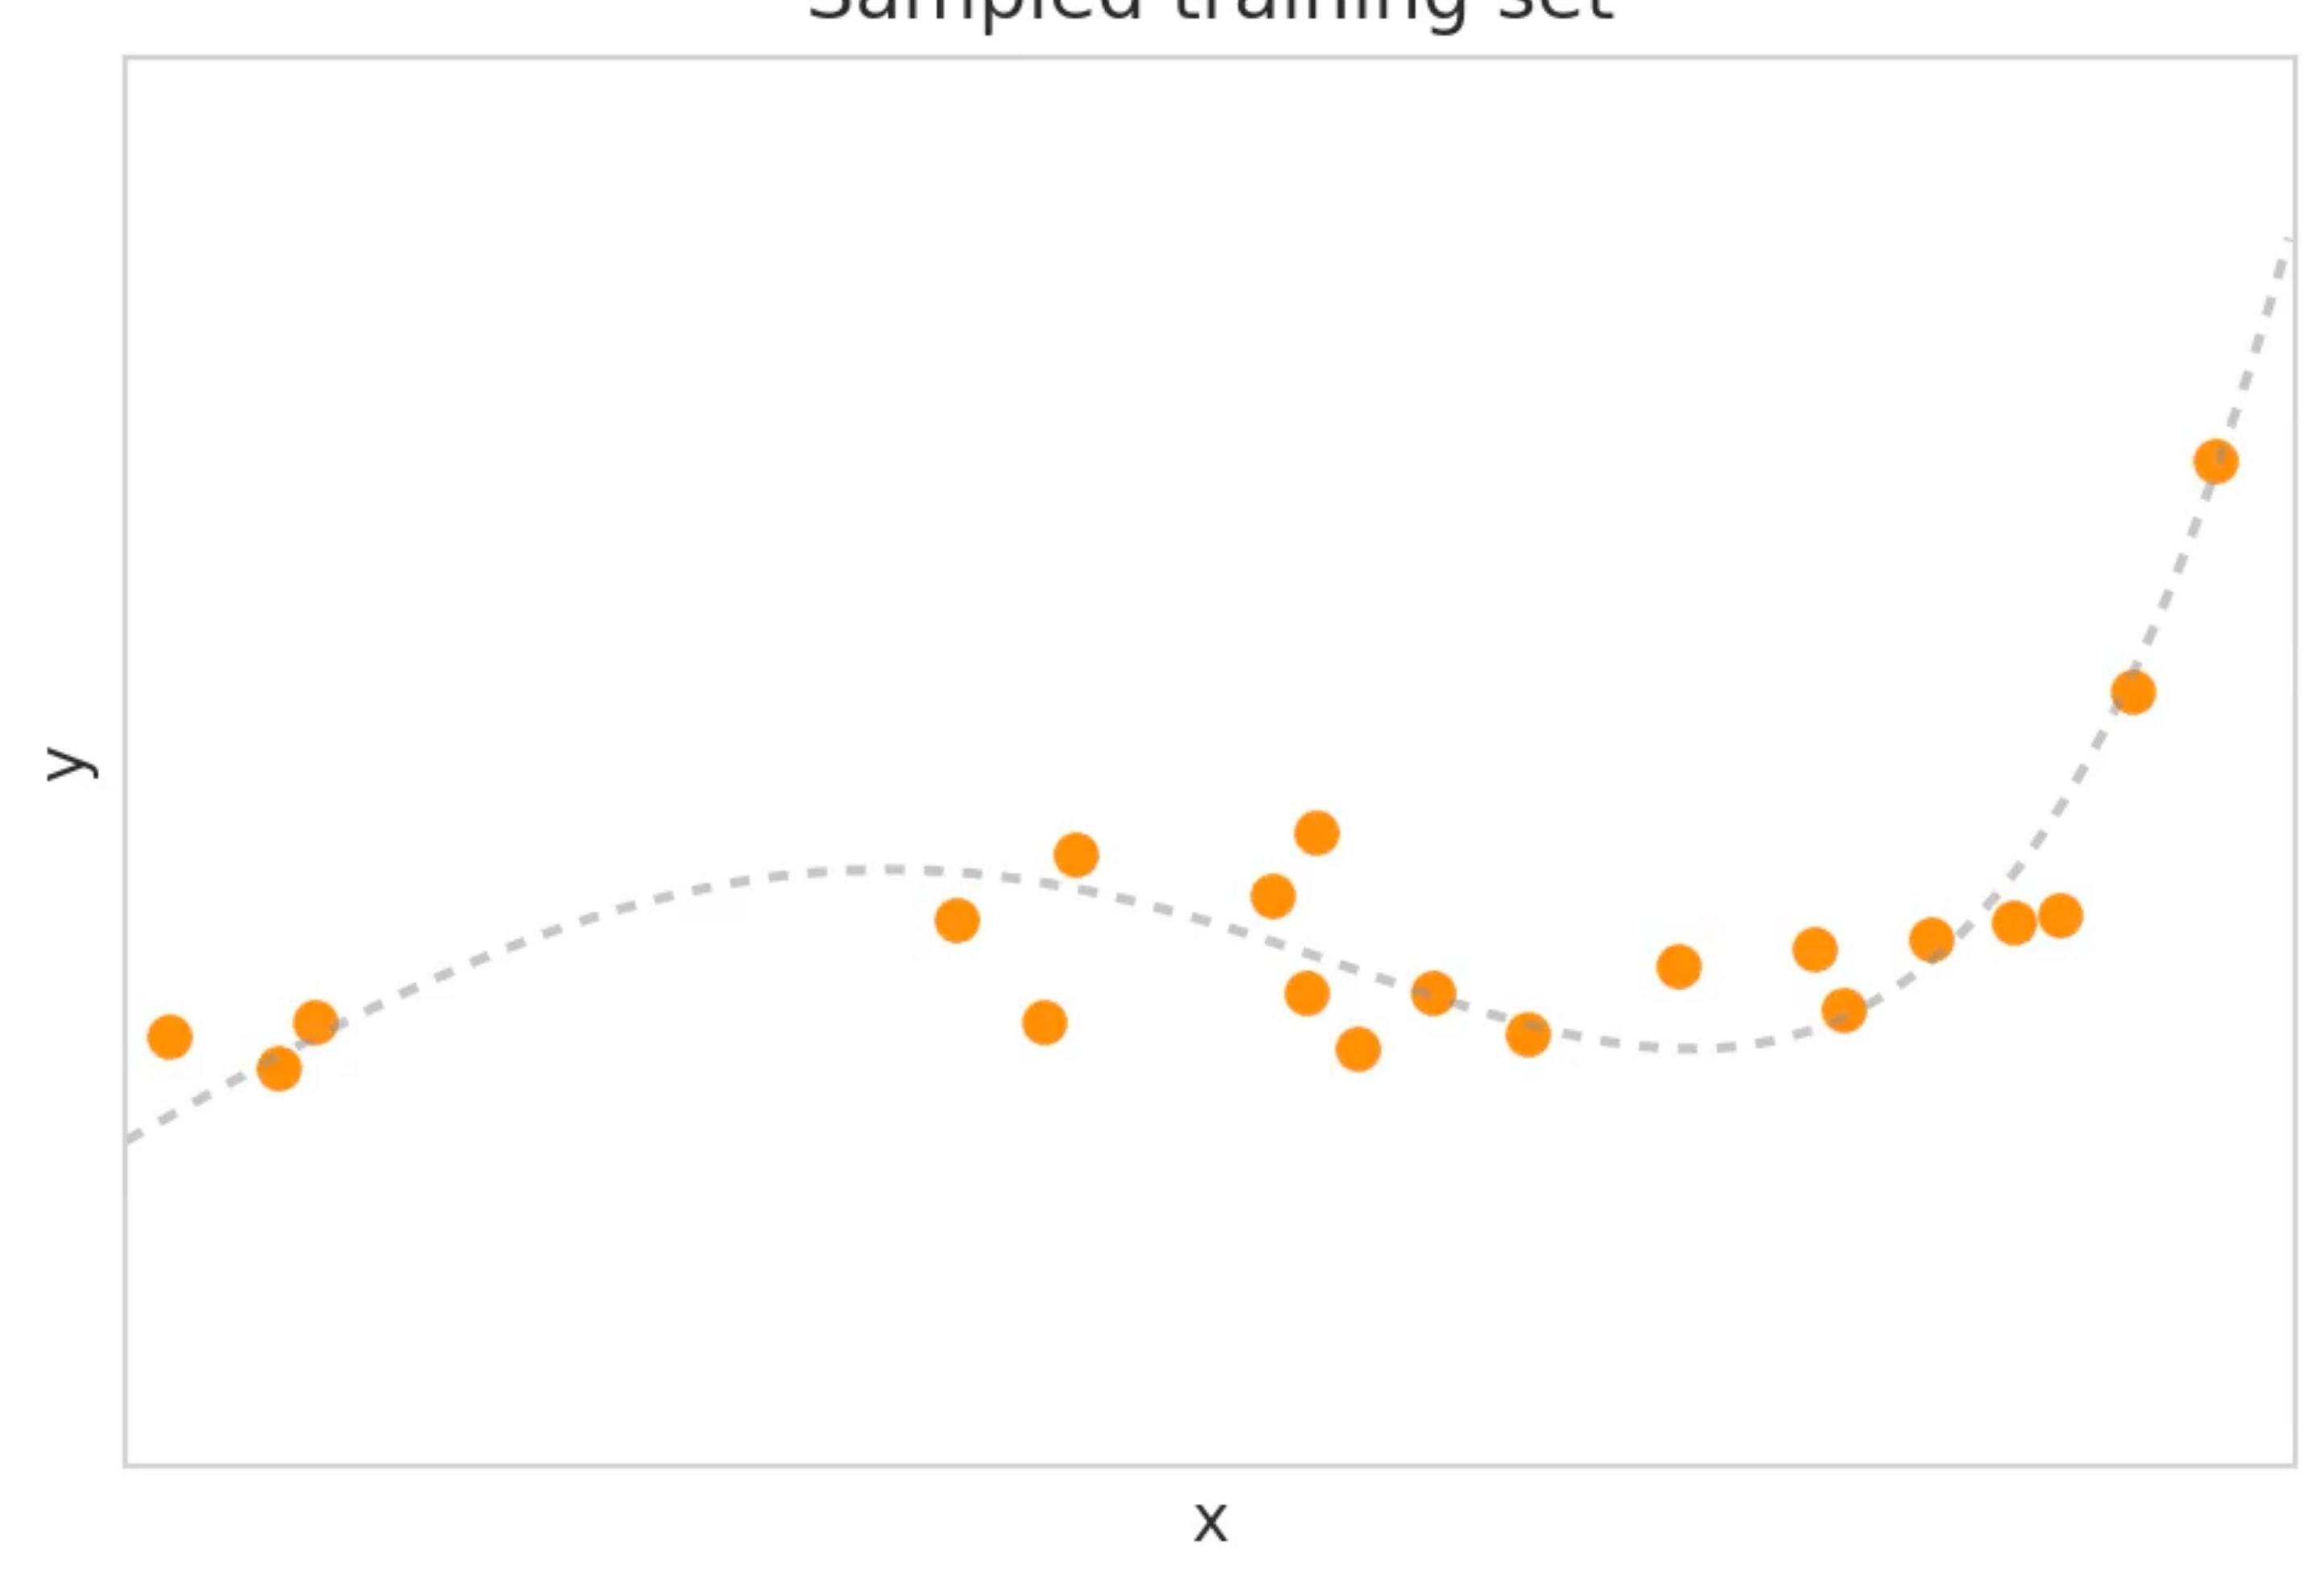
\includegraphics[max width=\textwidth]{2023_12_30_442f876157646883c2c9g-08}
\end{center}

We have observed one particular $S_{\text {train }}$ but we could have observed several others!

\section*{But there is randomness in the data}
Sampled training set

\begin{center}
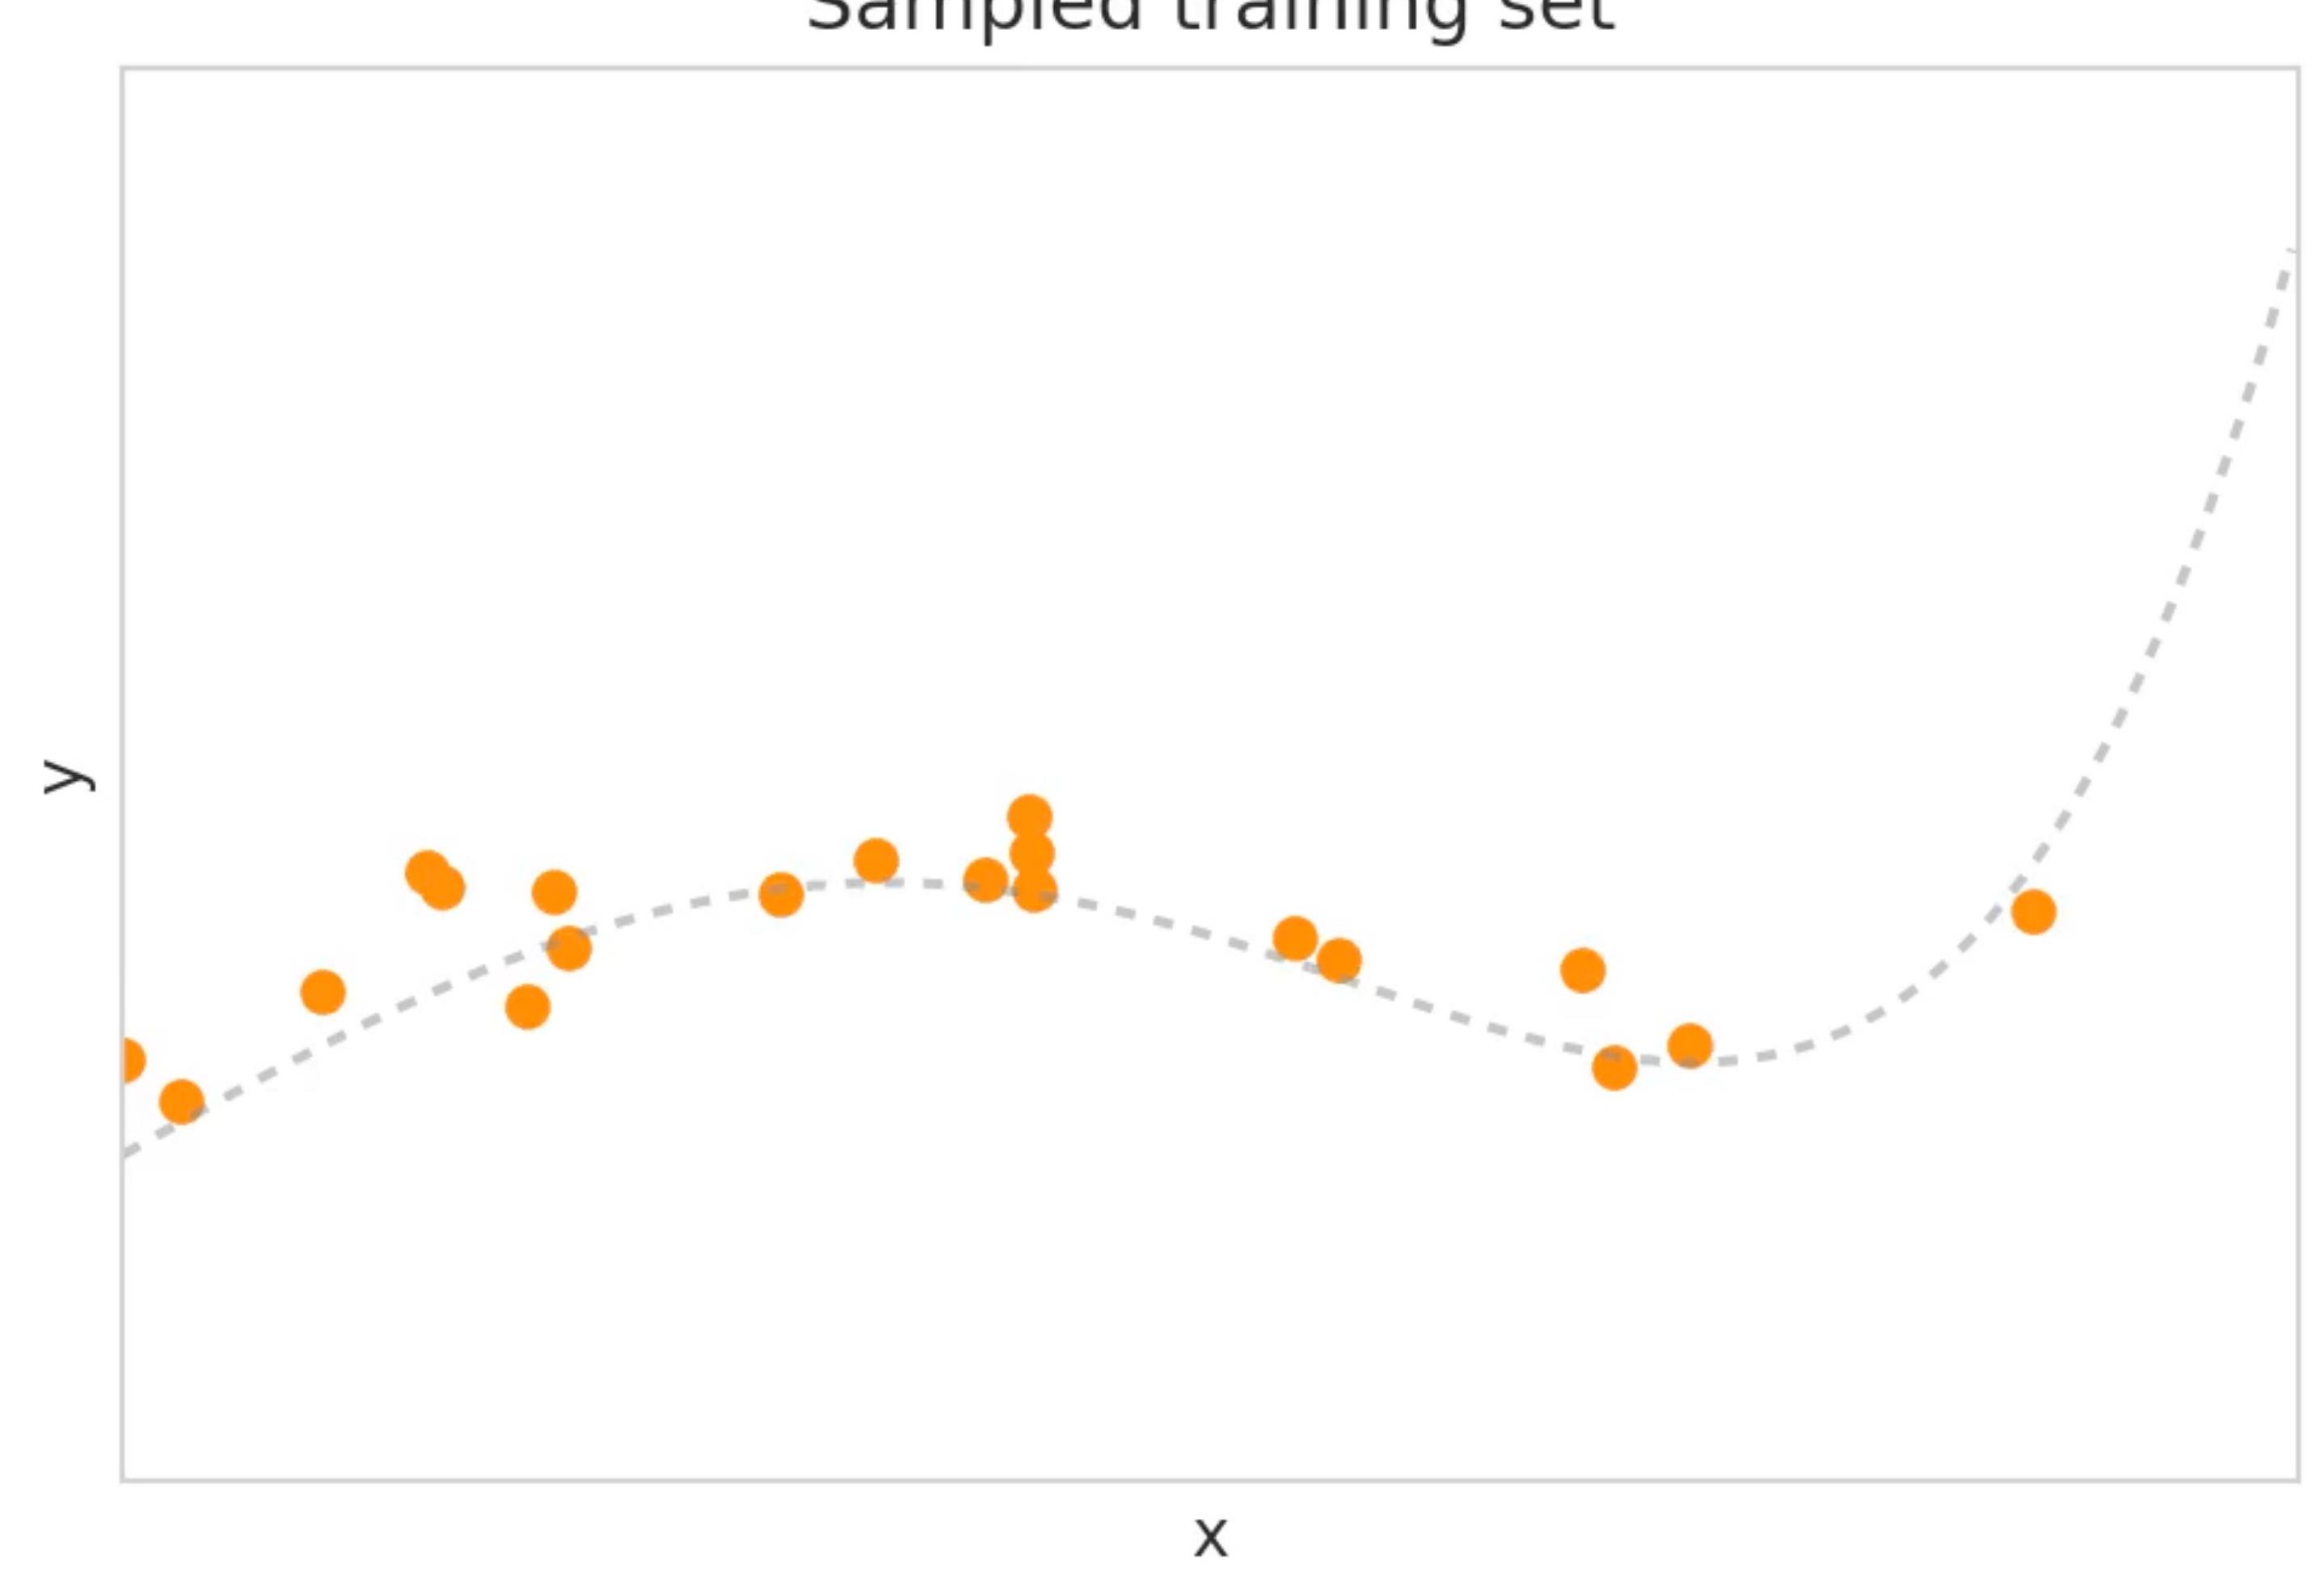
\includegraphics[max width=\textwidth]{2023_12_30_442f876157646883c2c9g-09}
\end{center}

Even if we keep the same $\left(x_{1}, \cdots, x_{n}\right)$, we have variability in the observed $\left(y_{1}, \cdots, y_{n}\right)$

\section*{Thus there is randomness in the predictions}
Training fit (degree 1)

\begin{center}
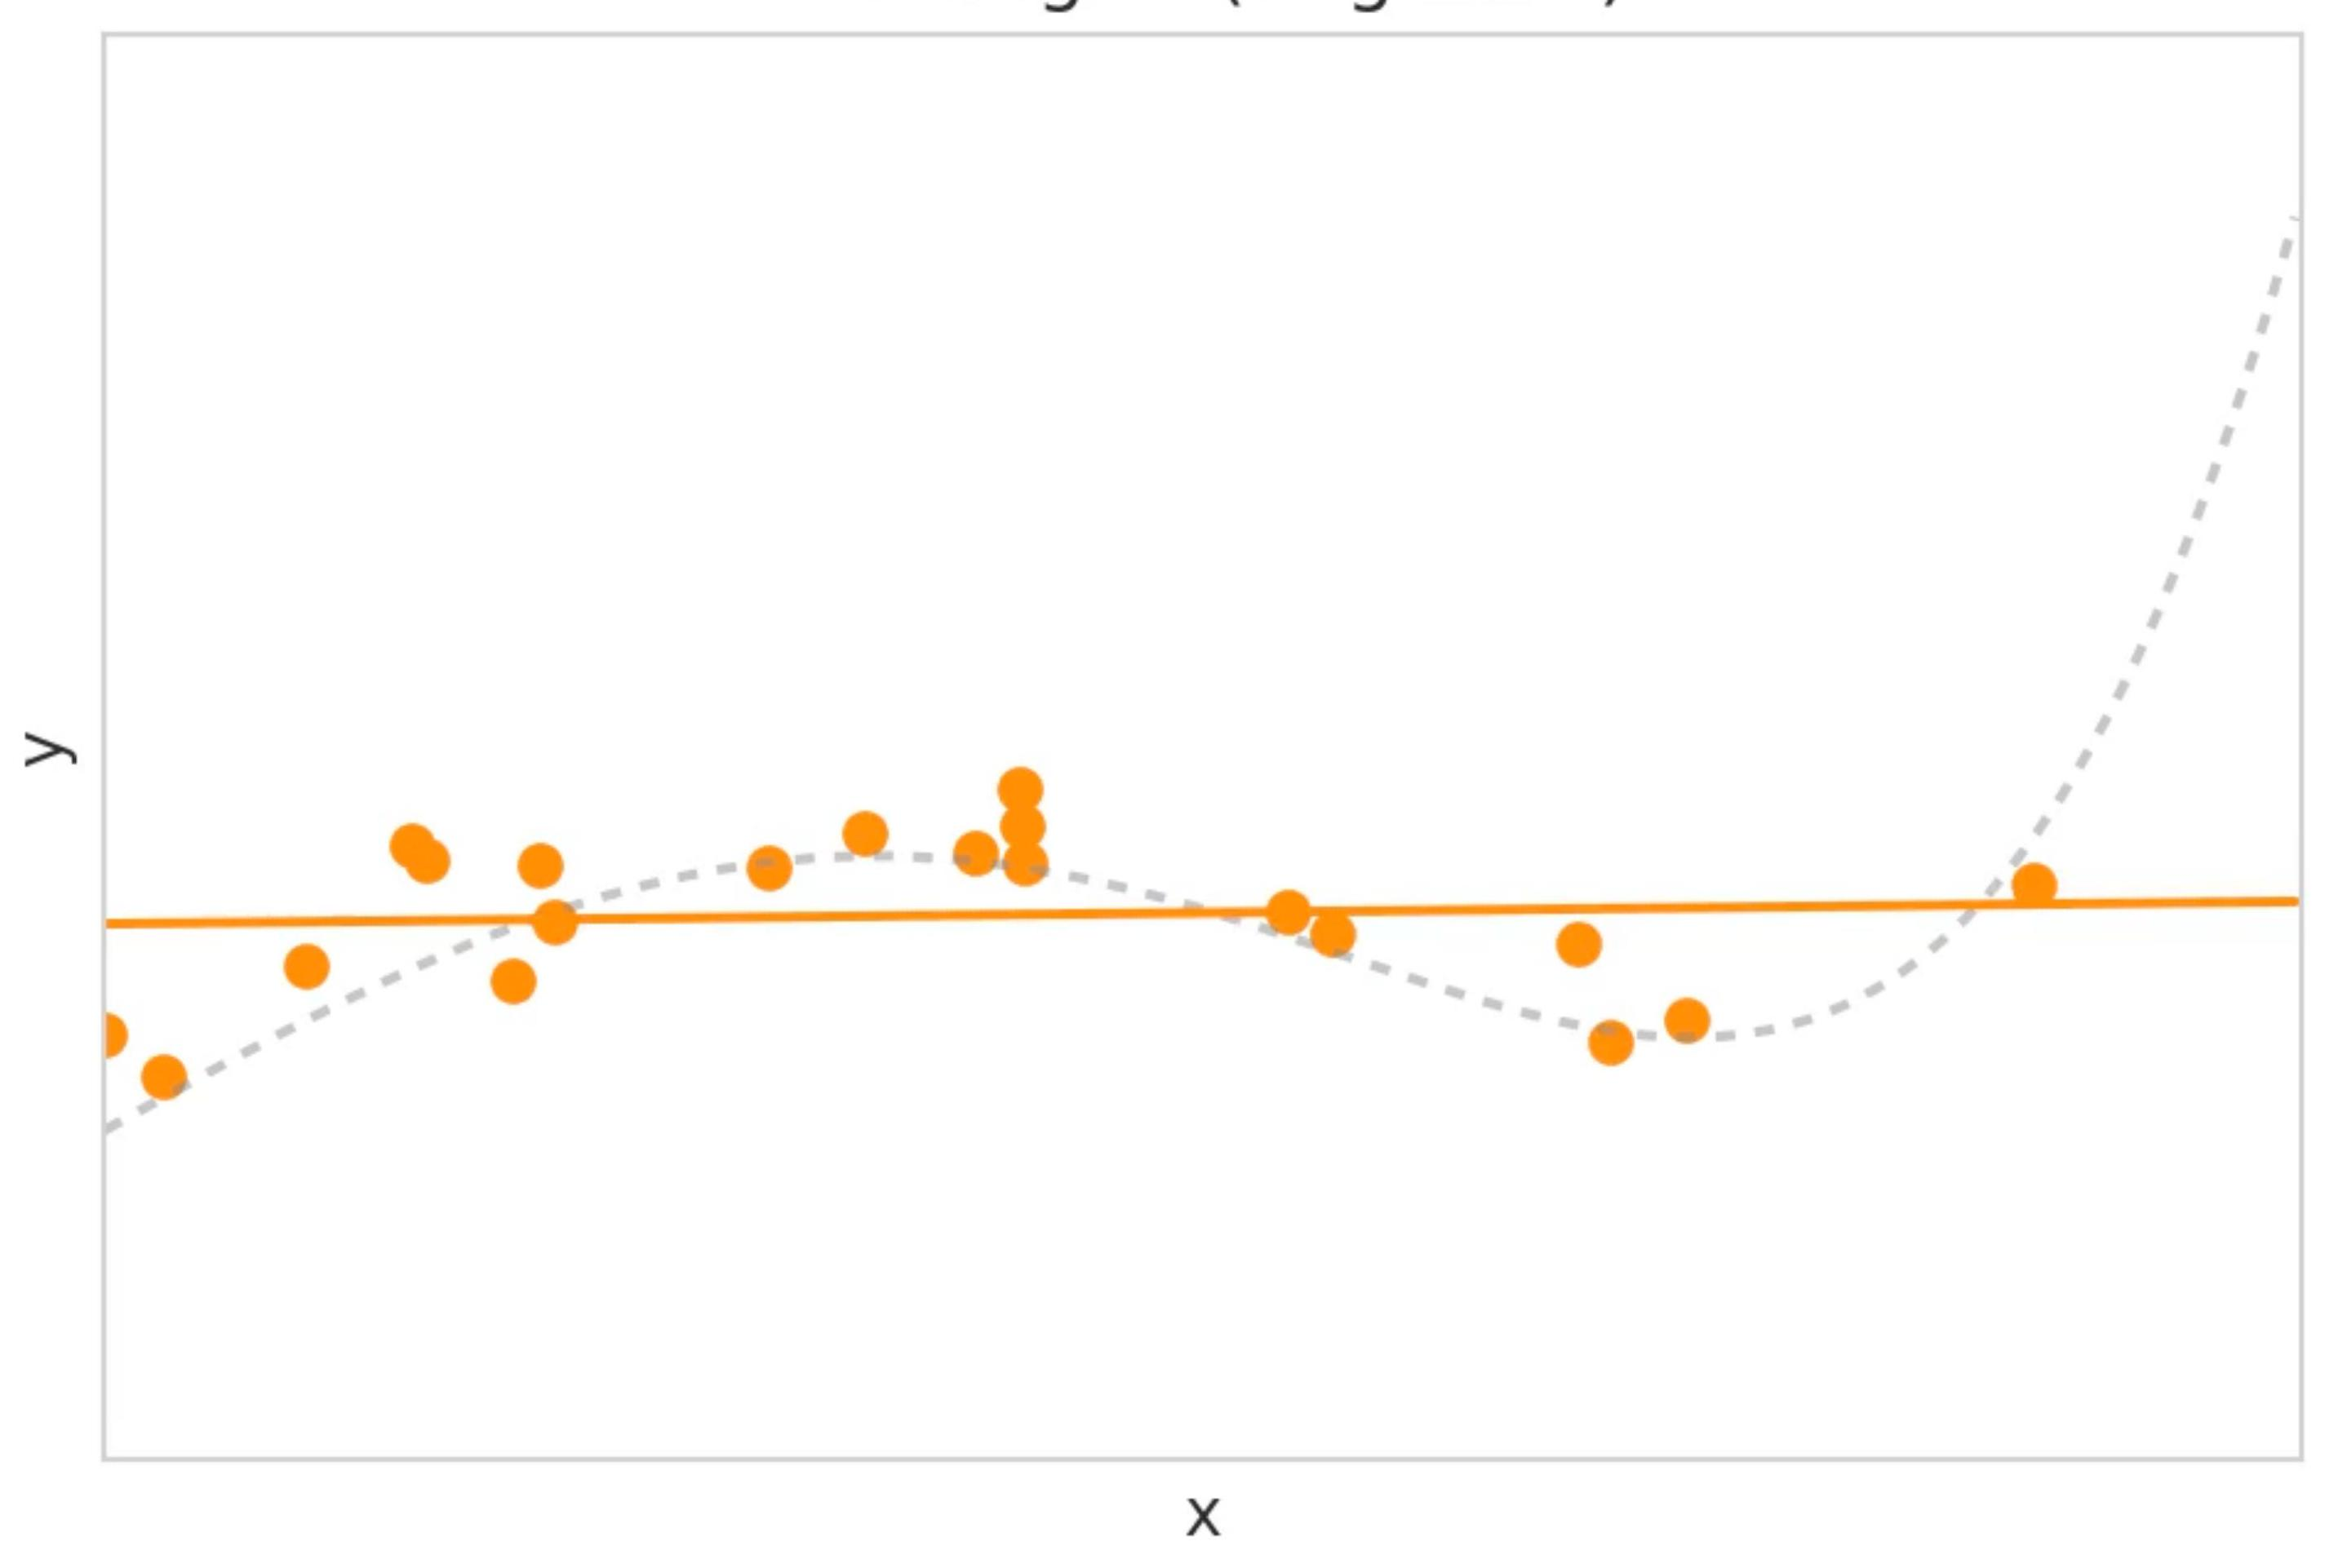
\includegraphics[max width=\textwidth]{2023_12_30_442f876157646883c2c9g-10(1)}
\end{center}

Moving a single observation will cause only a small shift in the position of the line

Underfitting
Training fit (degree 12)

\begin{center}
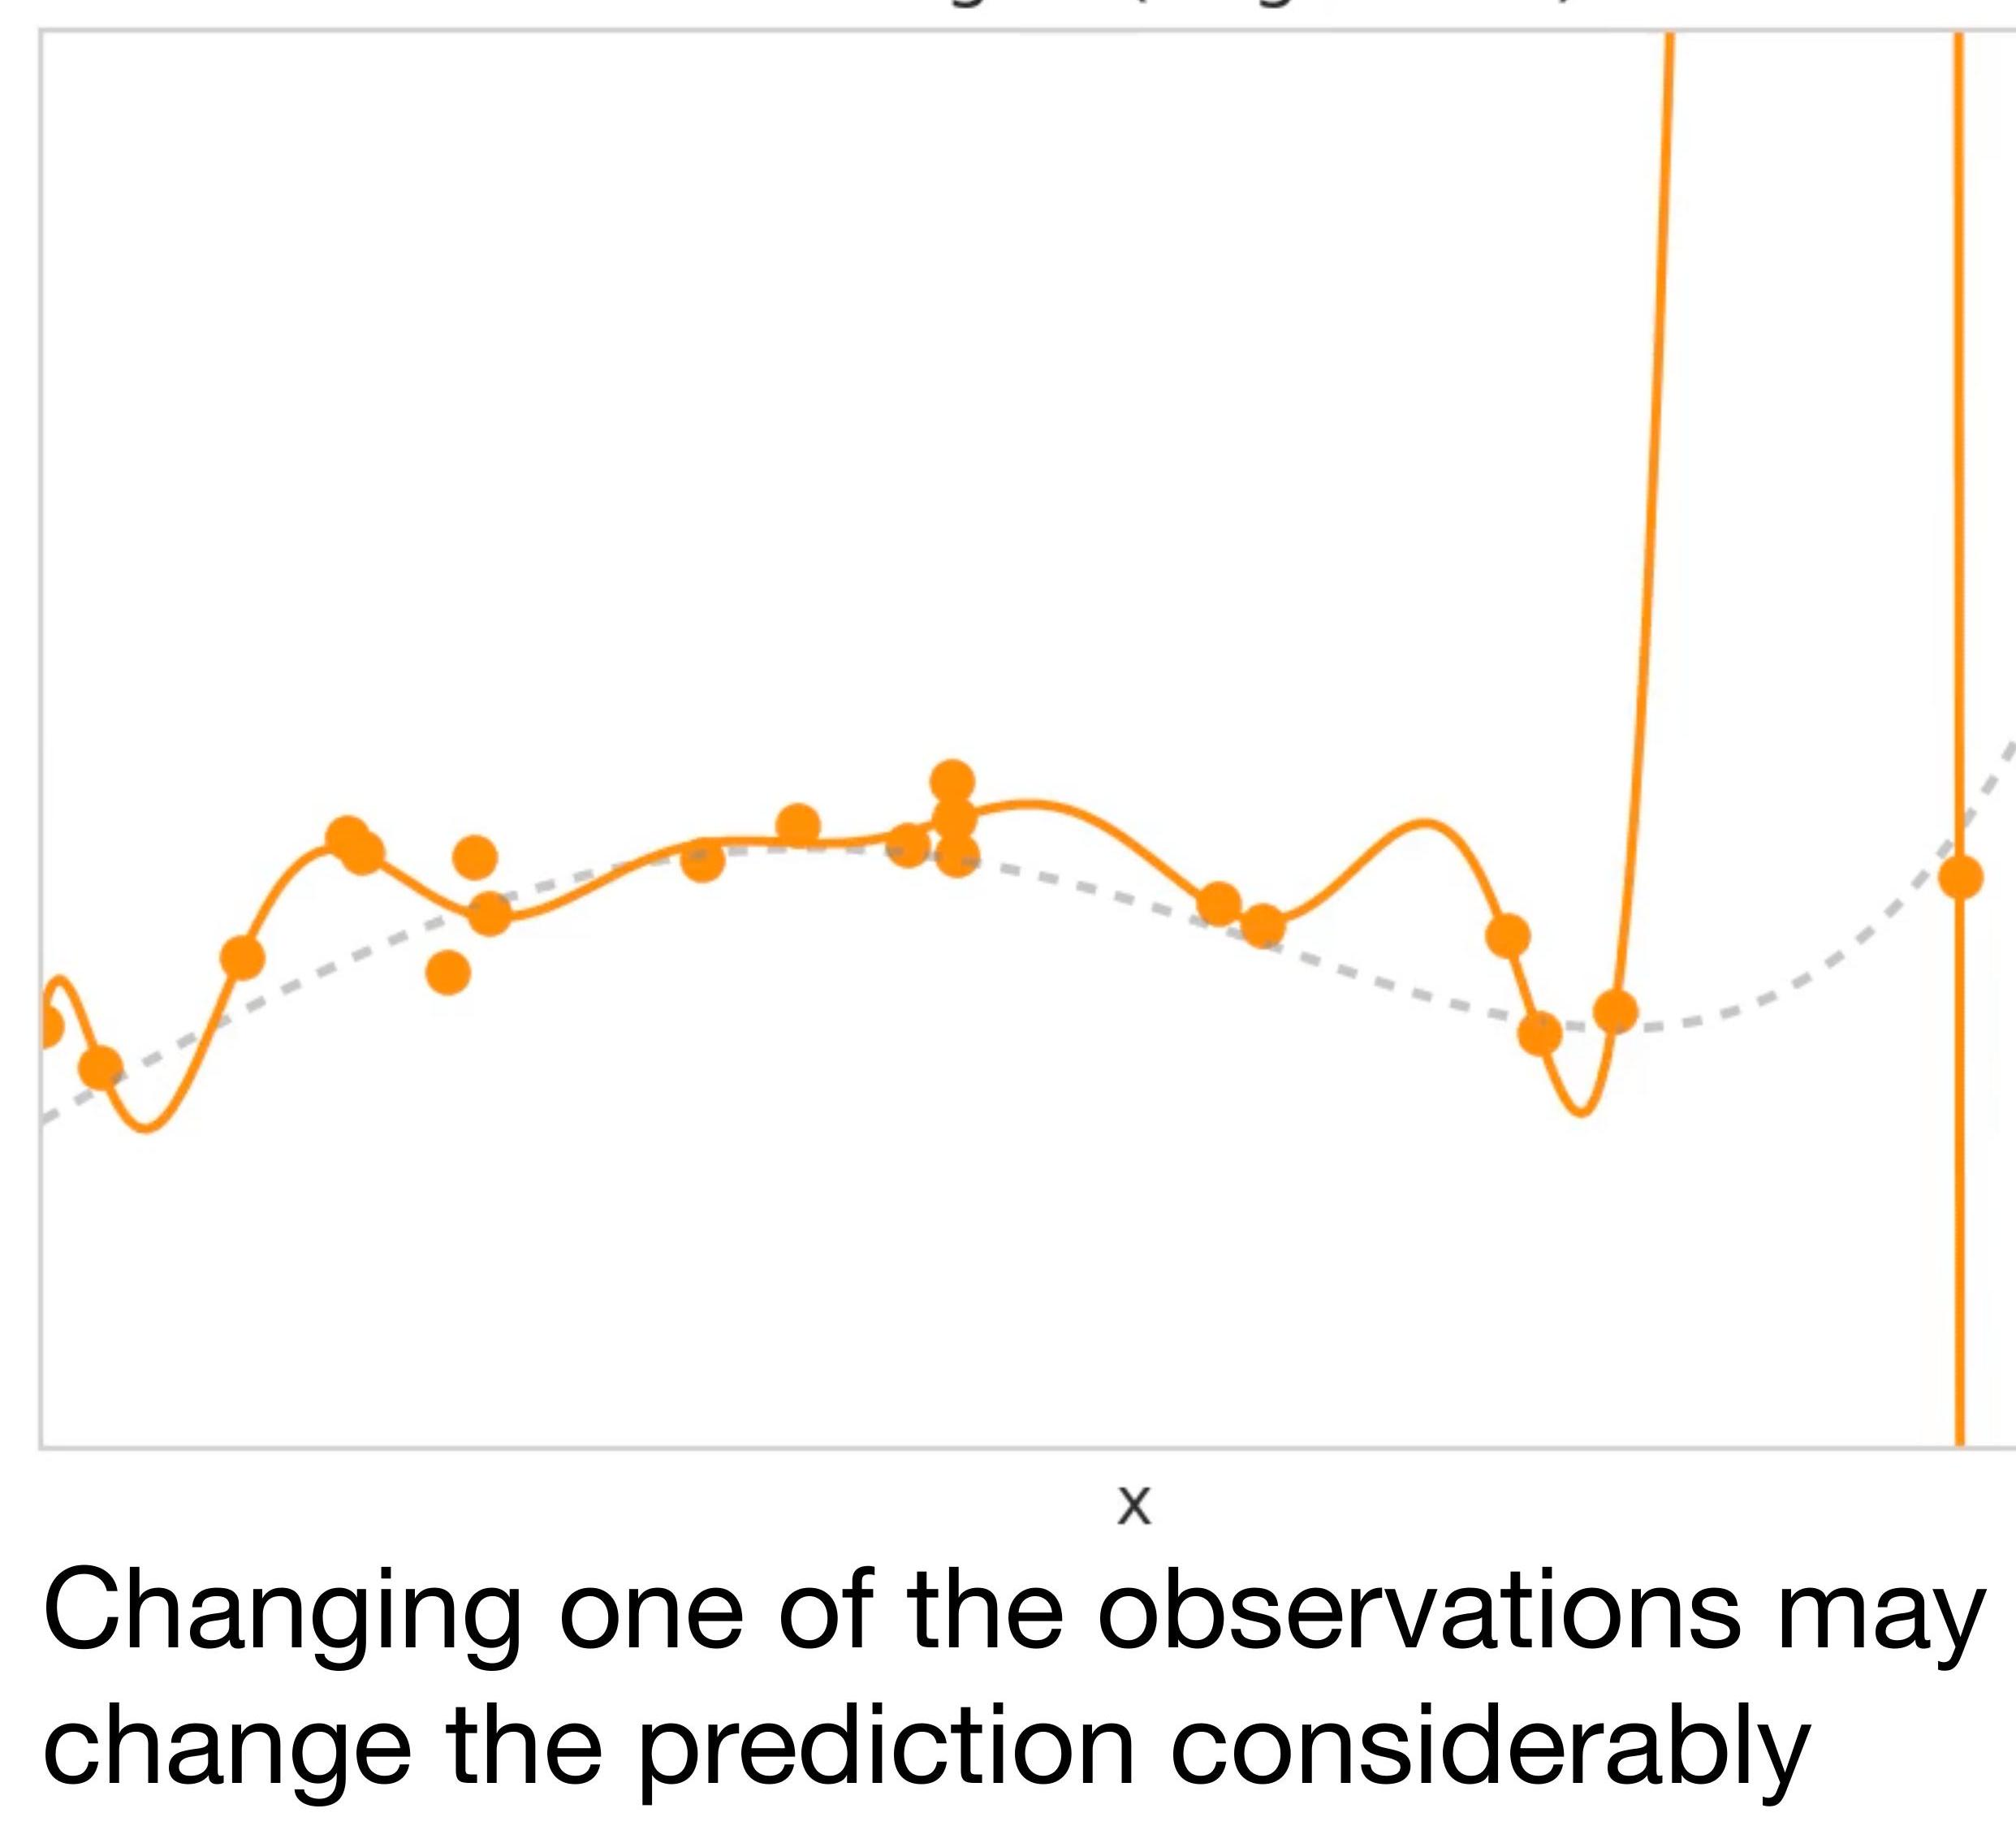
\includegraphics[max width=\textwidth]{2023_12_30_442f876157646883c2c9g-10}
\end{center}

Overfitting

Simple models are less sensitive

\section*{Simple models have large bias but low variance}
\begin{center}
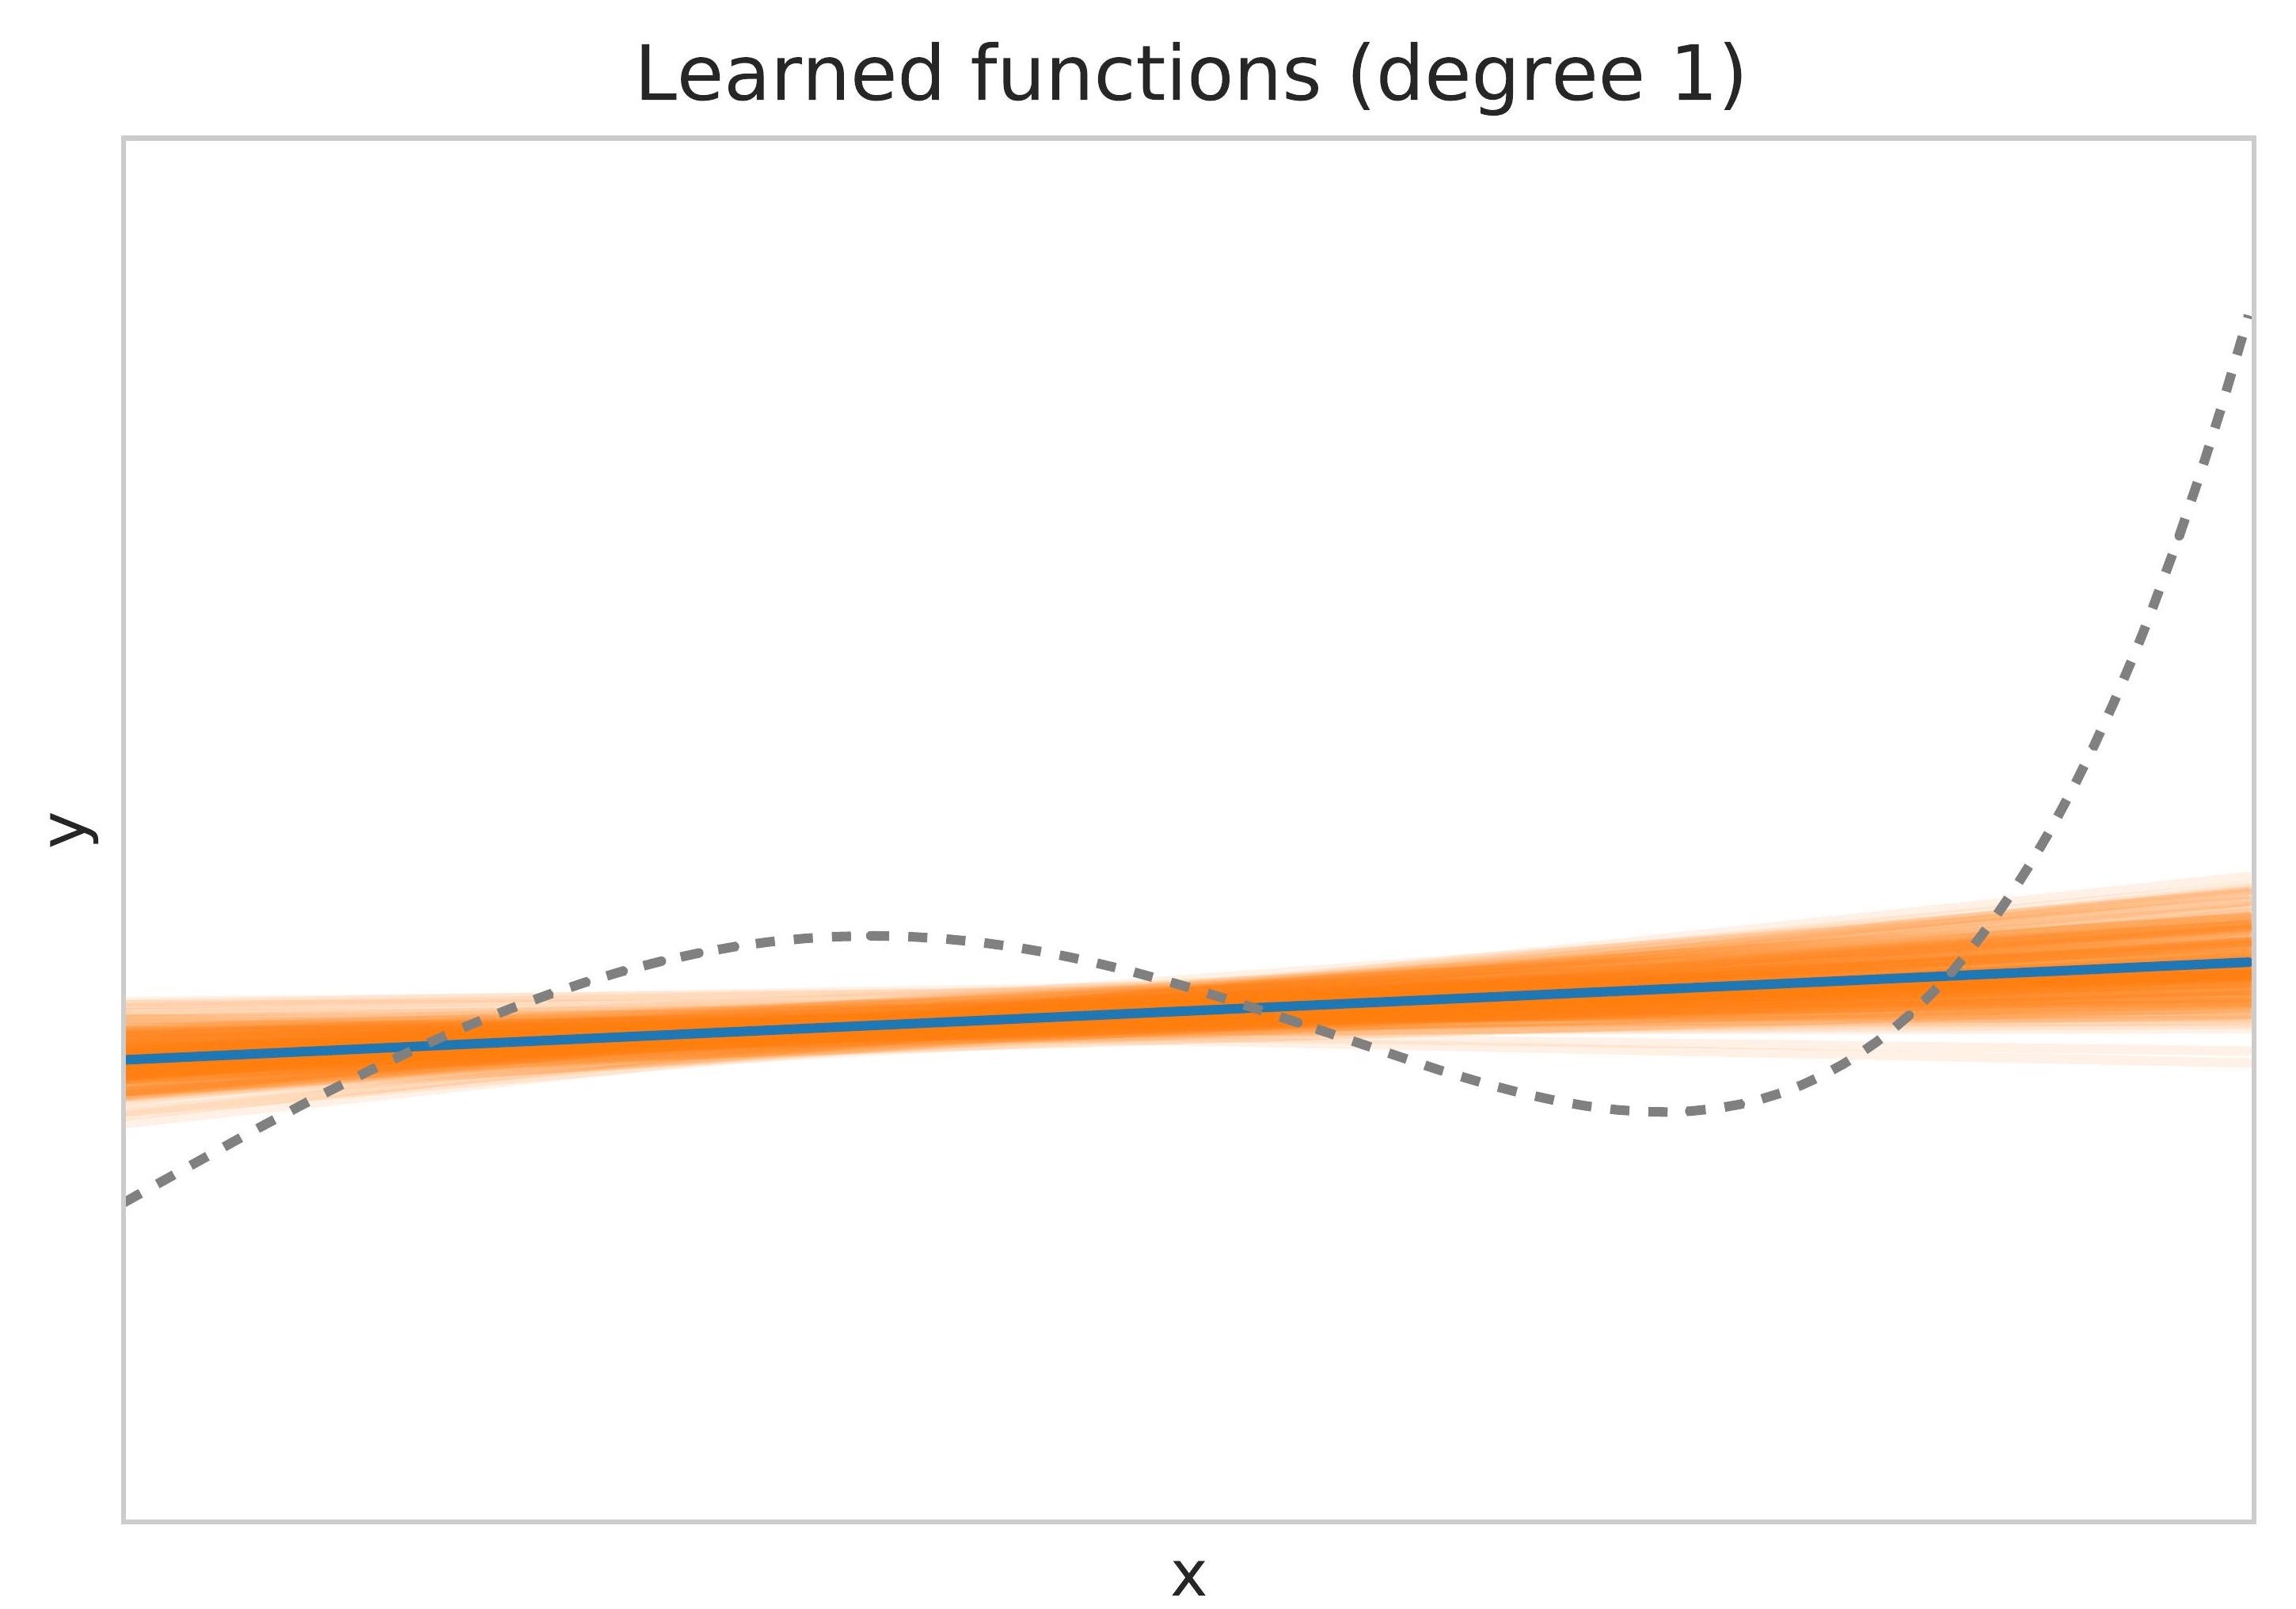
\includegraphics[max width=\textwidth]{2023_12_30_442f876157646883c2c9g-11}
\end{center}

The average of the predictions $f_{S}$ does not fit well the data: large bias The variance of the predictions $f_{S}$ as a function of $S$ is small: small variance

\section*{Complex models have low bias but high variance}
\begin{center}
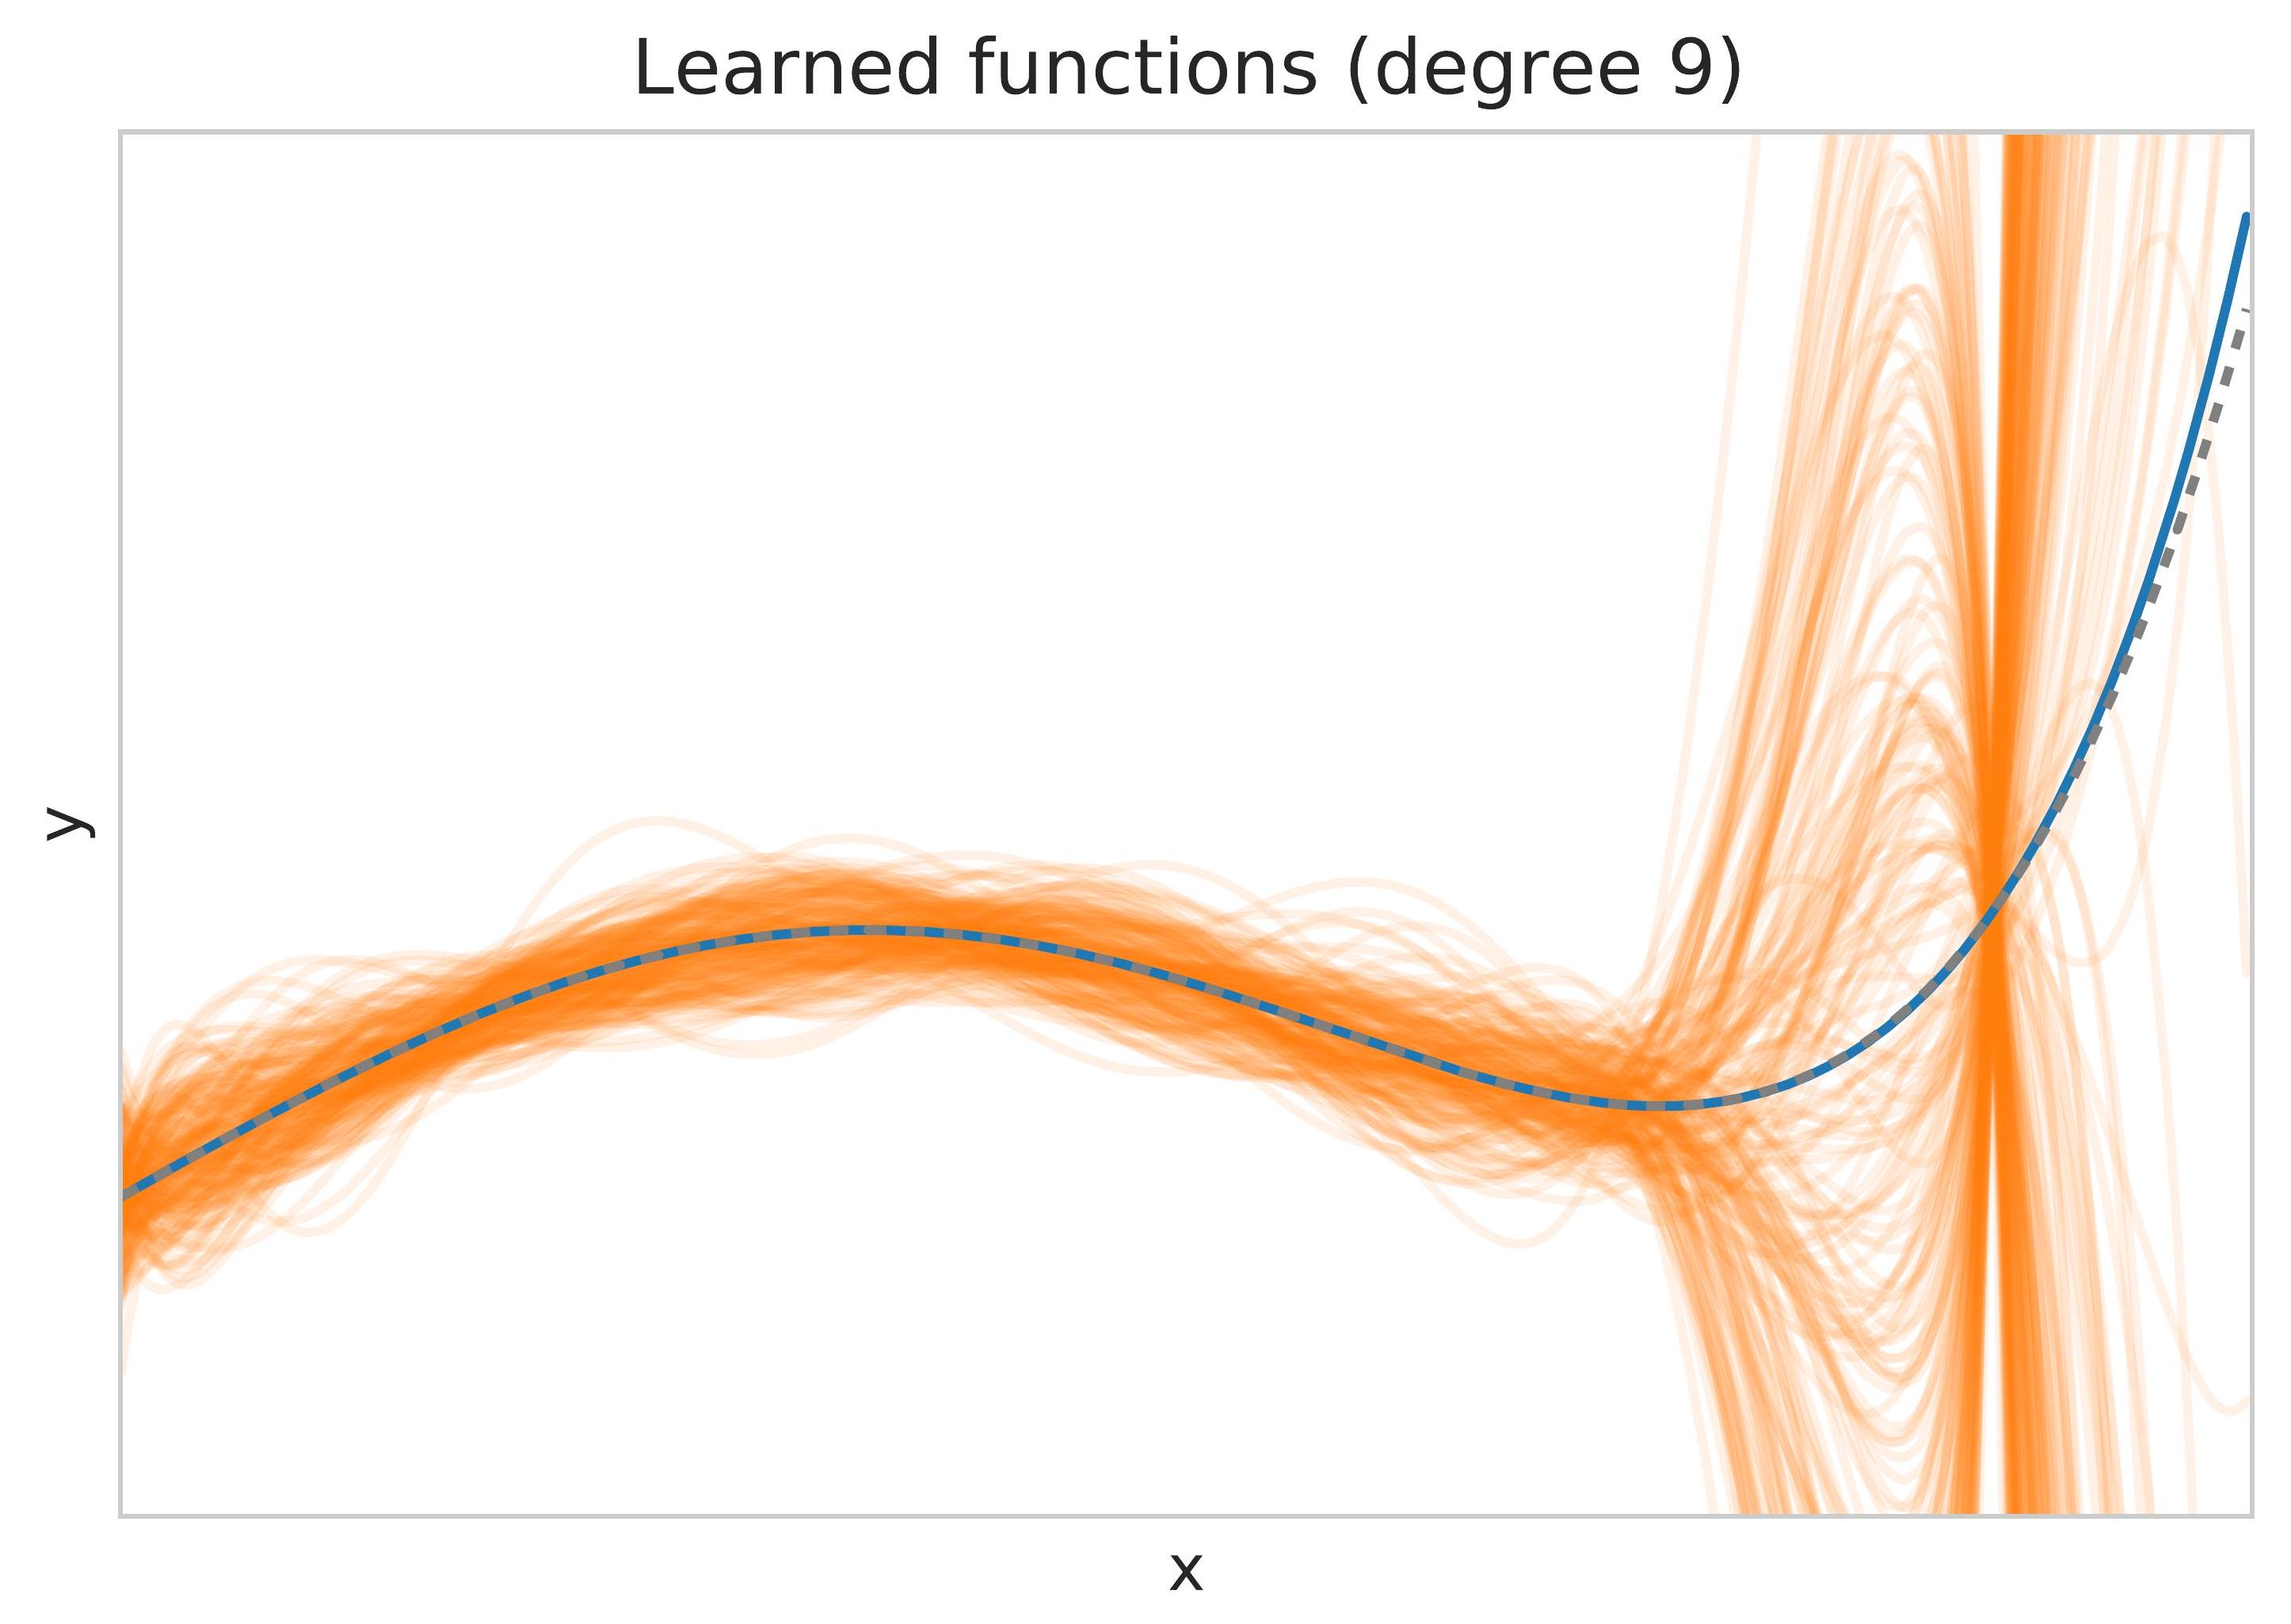
\includegraphics[max width=\textwidth]{2023_12_30_442f876157646883c2c9g-12}
\end{center}

The average of the predictions $f_{S}$ fits well the data: small bias

The variance of the predictions $f_{S}$ as a function of $S$ is large: large variance

\section*{We need to balance bias \& variance correctly}
\begin{center}
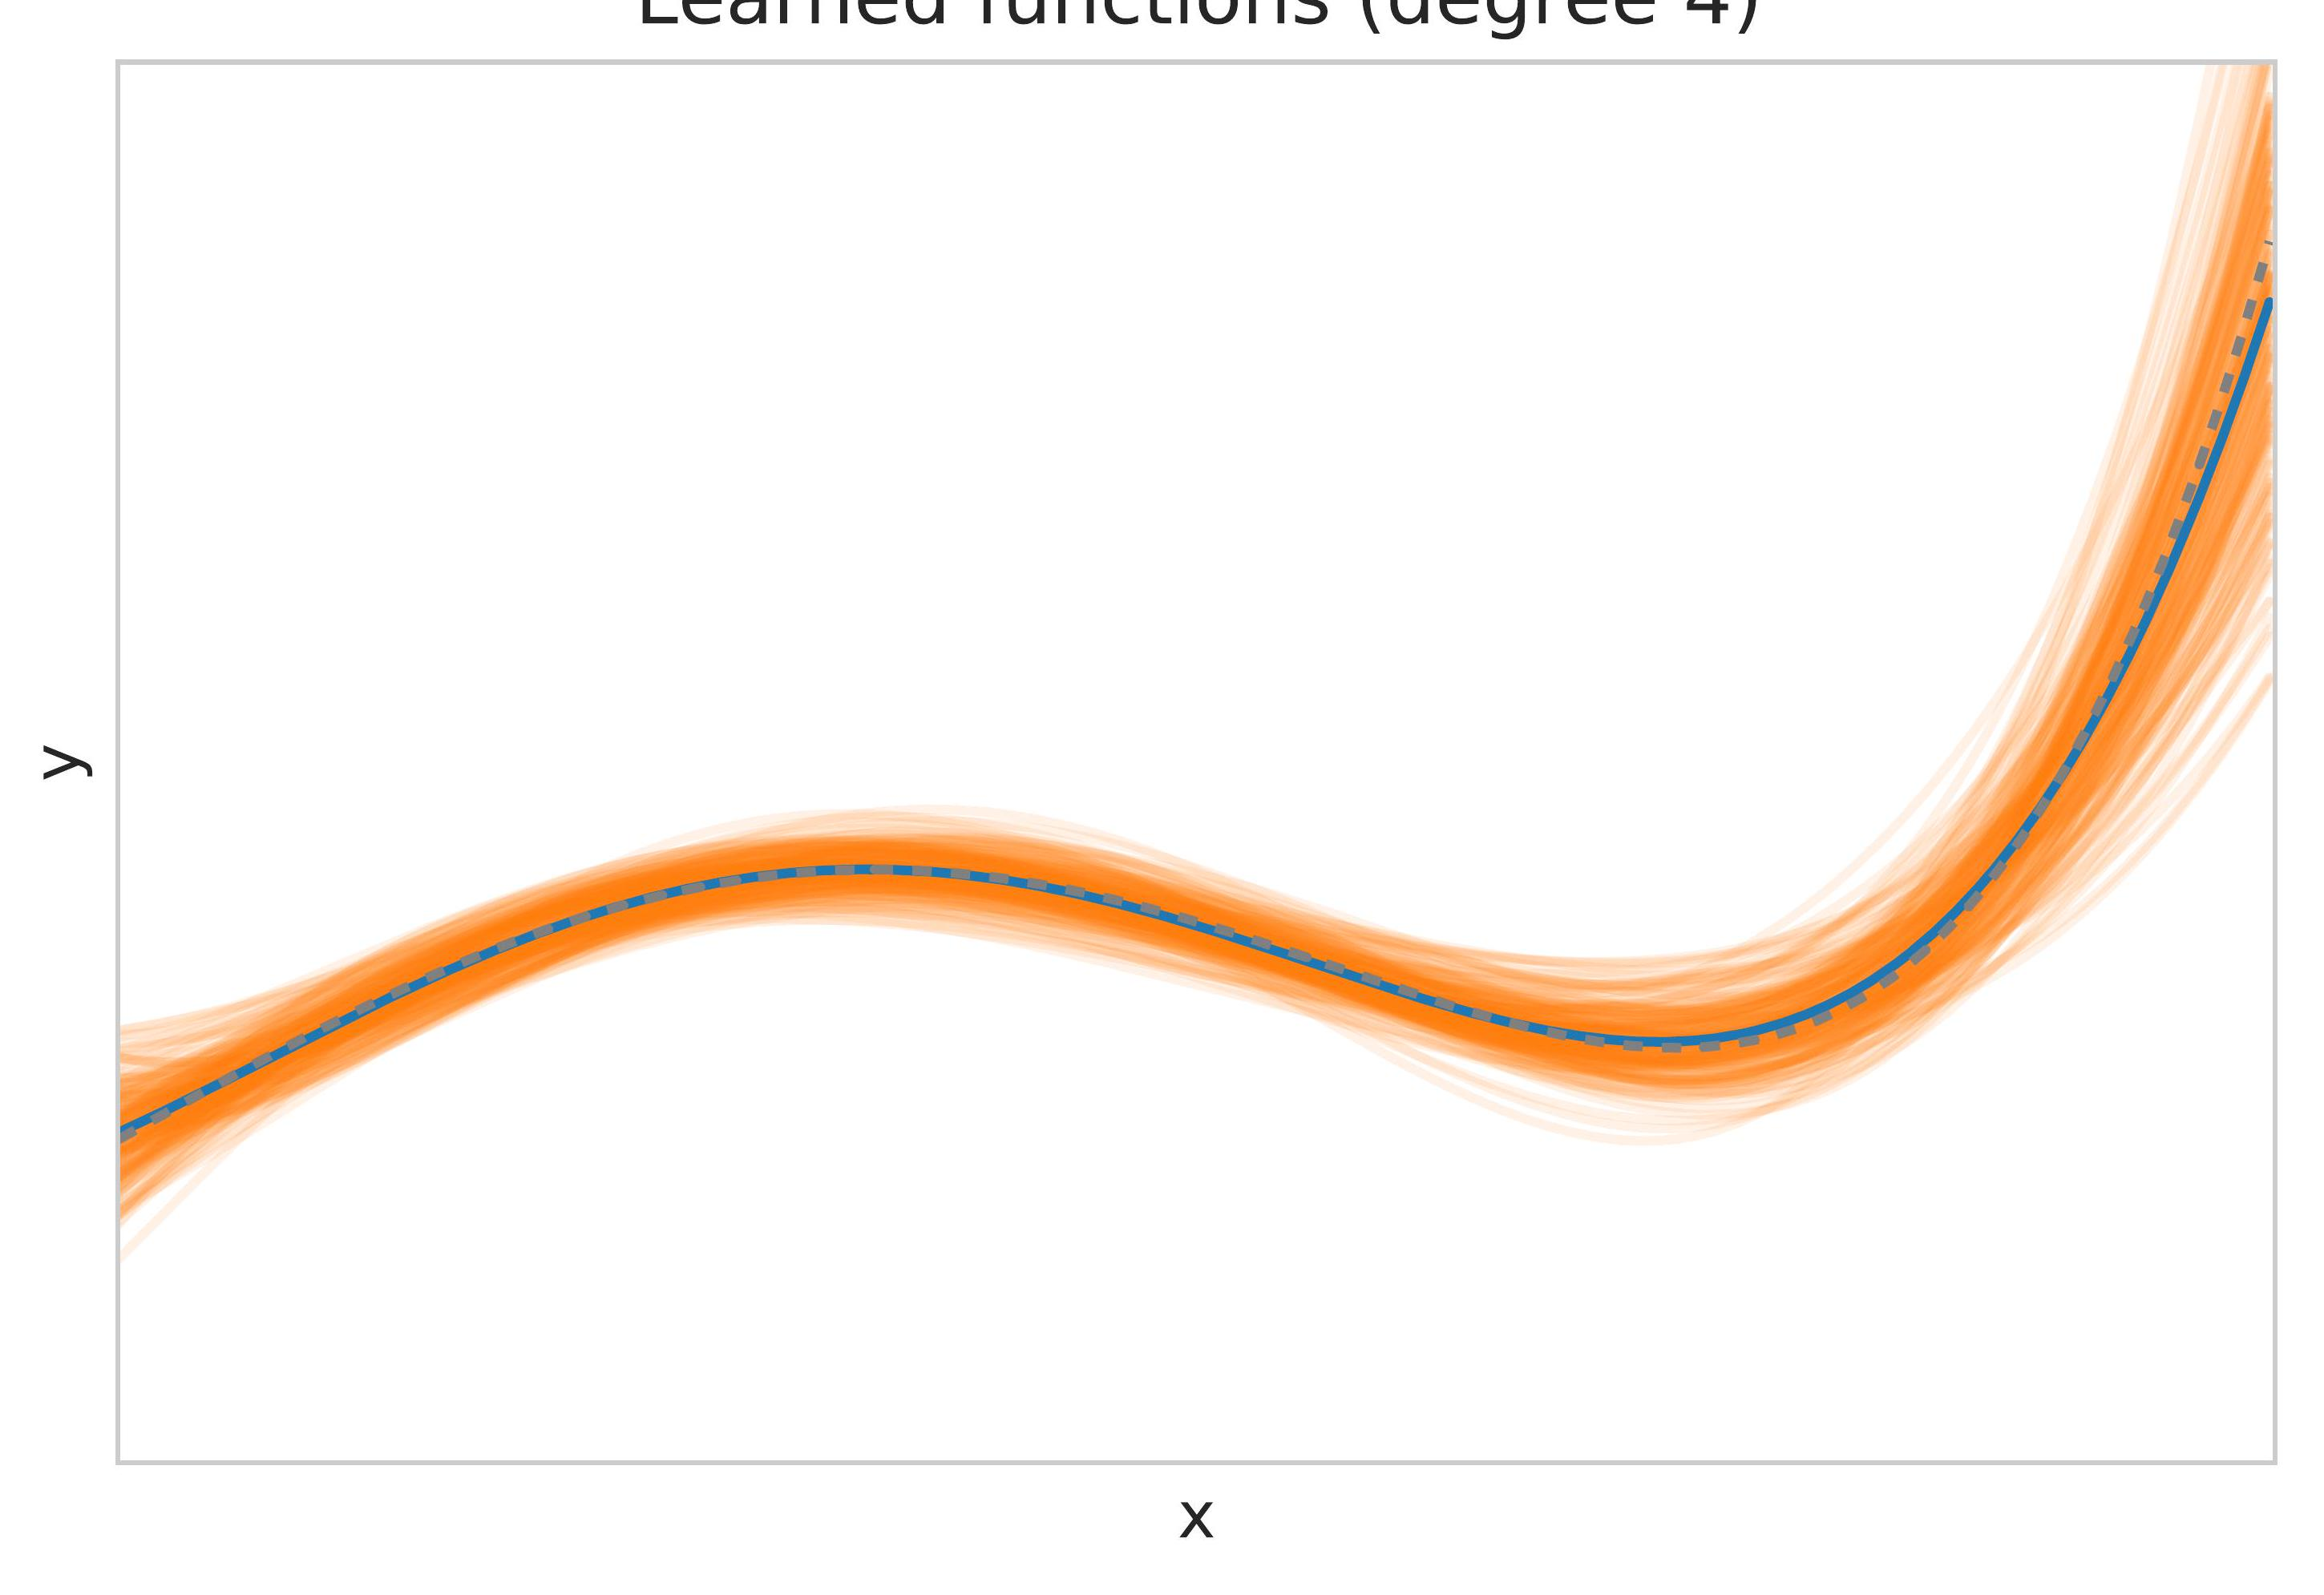
\includegraphics[max width=\textwidth]{2023_12_30_442f876157646883c2c9g-13}
\end{center}

\section*{Data model: output perturbed by some noise}
\begin{center}
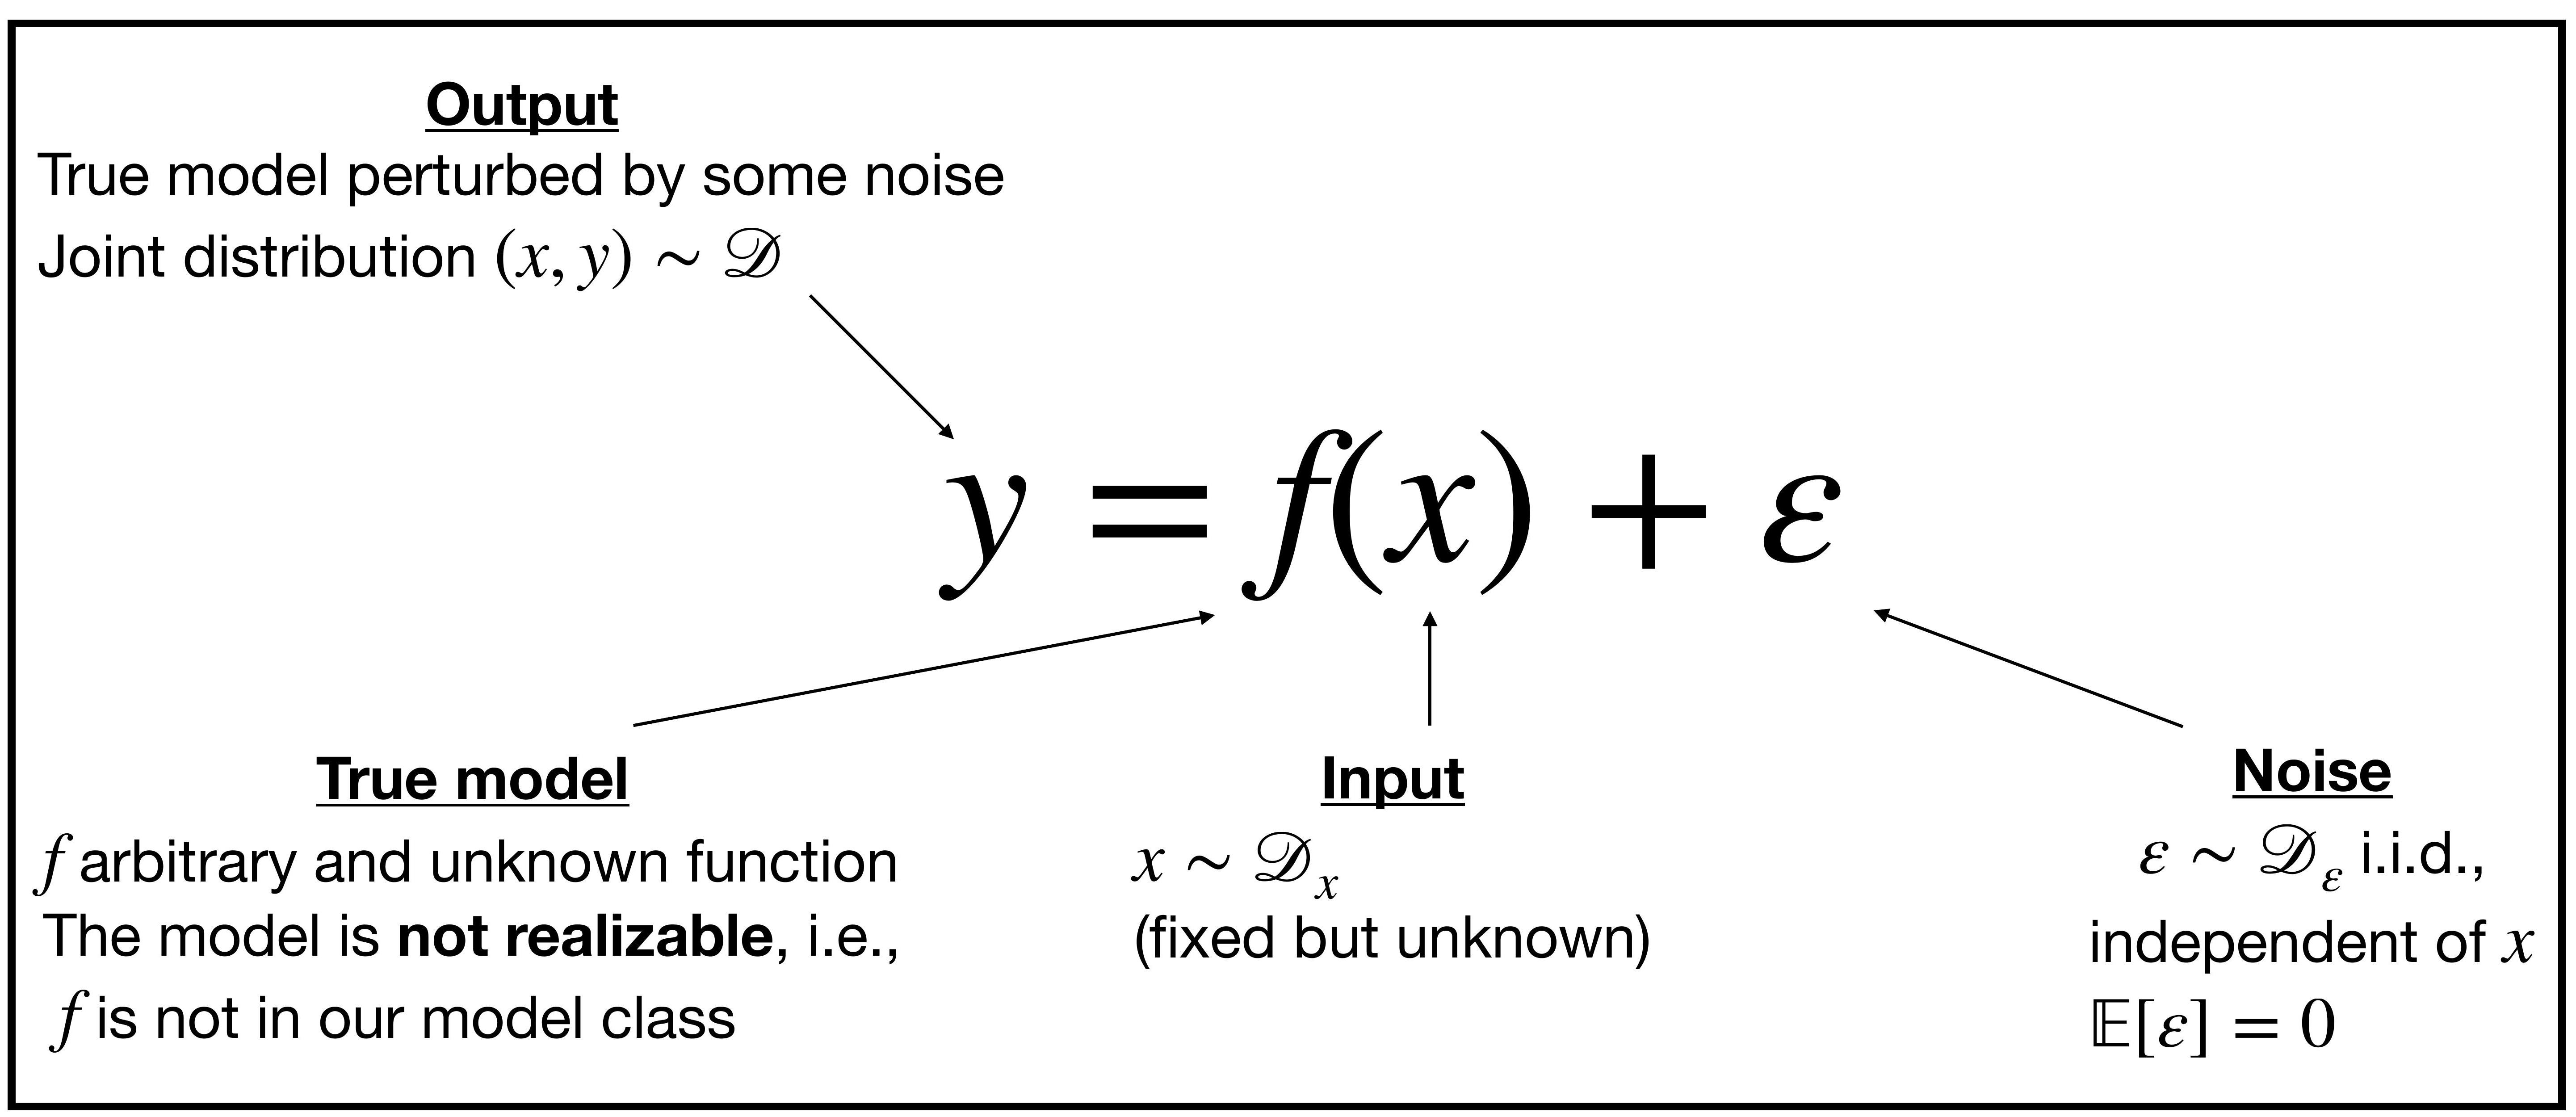
\includegraphics[max width=\textwidth]{2023_12_30_442f876157646883c2c9g-14}
\end{center}

We consider the square loss and will provide a decomposition of the true error

\section*{Error Decomposition}
\begin{center}
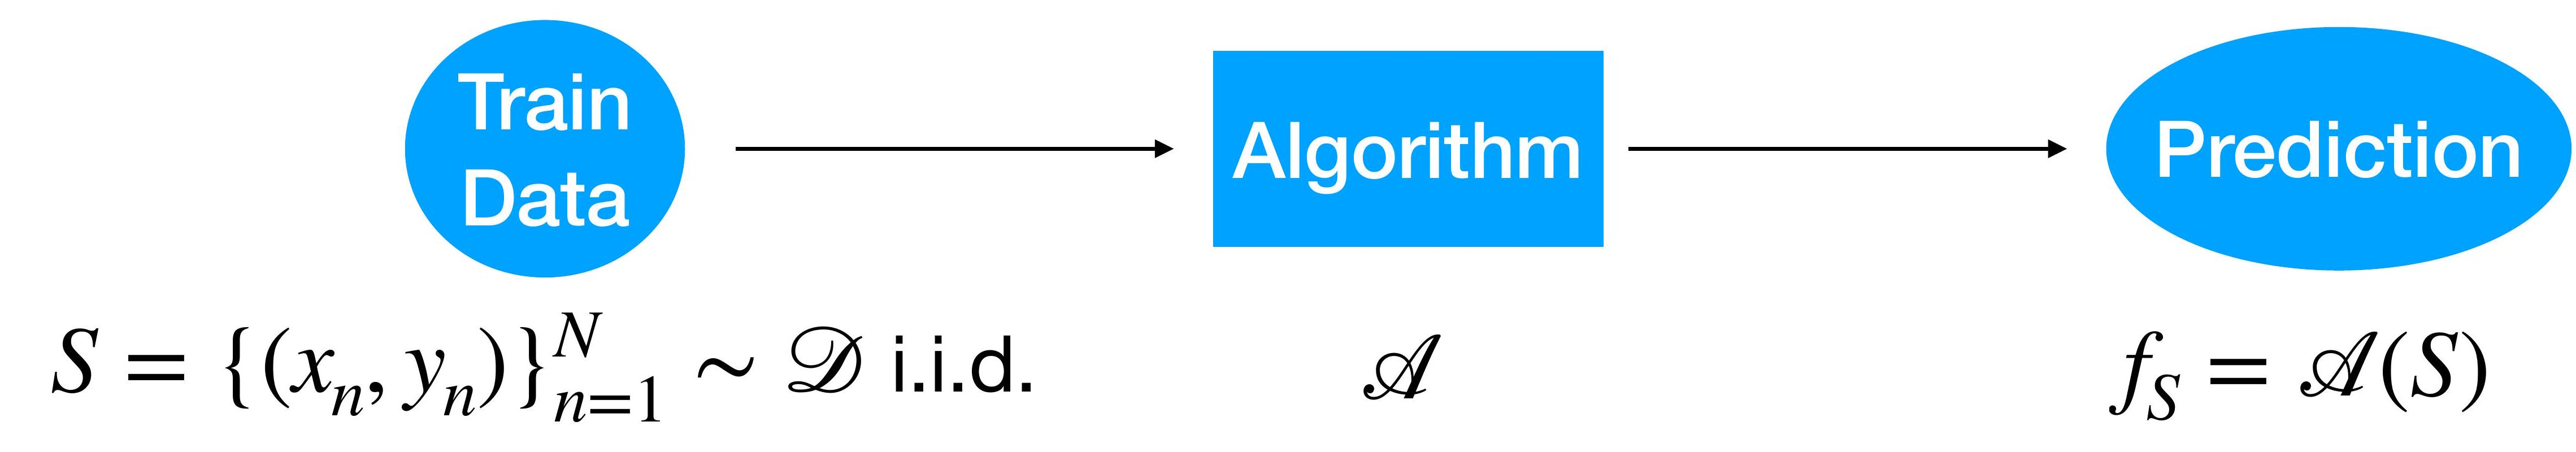
\includegraphics[max width=\textwidth]{2023_12_30_442f876157646883c2c9g-15}
\end{center}

We are interested in how the expected error of $f_{S}$ :

$$
\mathbb{E}_{(x, y) \sim D}\left[\left(y-f_{S}(x)\right)^{2}\right]
$$

behaves as a function of the train set $S$ and model class complexity

\section*{Error Decomposition}
\begin{center}
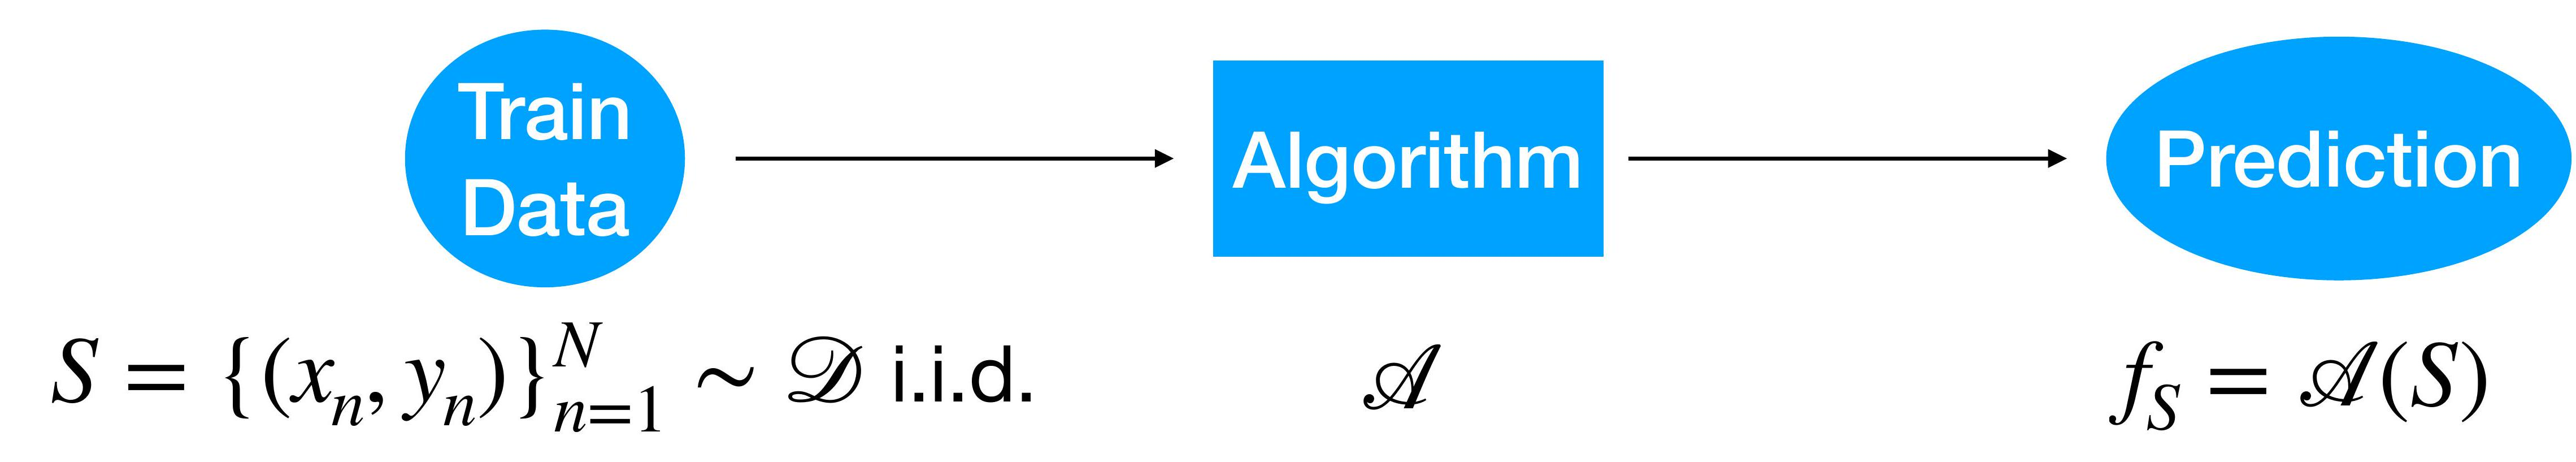
\includegraphics[max width=\textwidth]{2023_12_30_442f876157646883c2c9g-16}
\end{center}

The decomposition will hold true at every single point $x$. Therefore, to simplify, we consider the expected error of $f_{S}$ for a fixed element $x_{0}$ :

$$
L\left(f_{S}\right)=\mathbb{E}_{\varepsilon \sim \mathscr{D}_{\varepsilon}}\left[\left(f\left(x_{0}\right)+\varepsilon-f_{S}\left(x_{0}\right)\right)^{2}\right]
$$

This is a random variable. The randomness comes for the train set $S$

\section*{We run the experiment many times}
\begin{center}
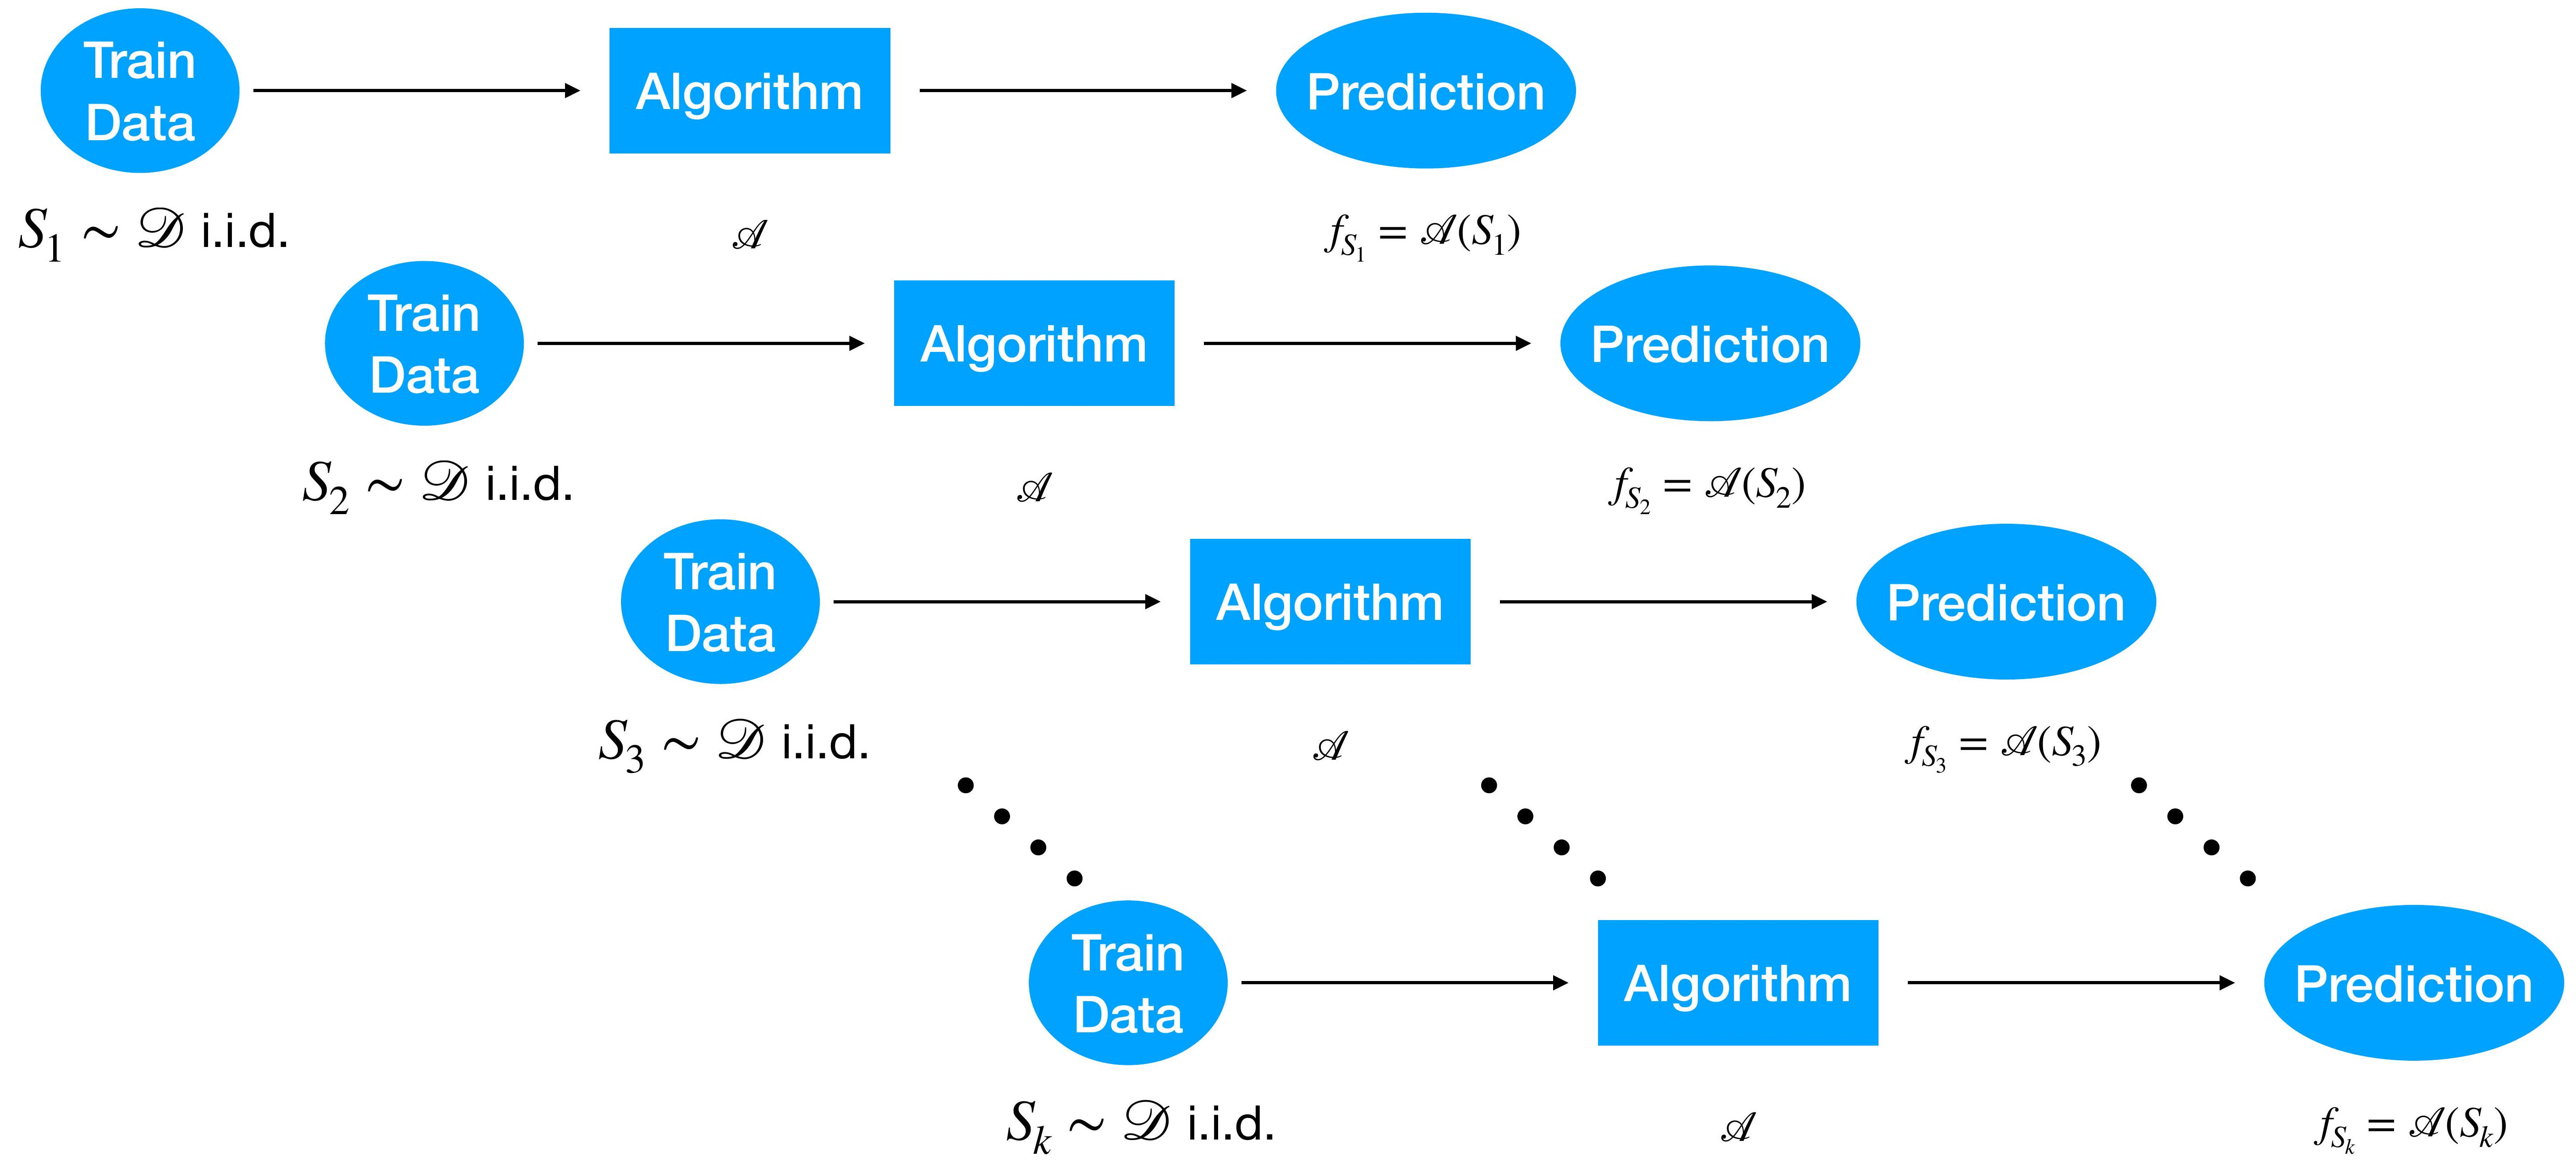
\includegraphics[max width=\textwidth]{2023_12_30_442f876157646883c2c9g-17}
\end{center}

We are interested in the average and the variance of the predictions $\left(f_{S_{1}}, \cdots, f_{S_{k}}\right)$ over these multiple runs

\section*{A decomposition in three terms}
We are interested in the expectation of the true risk over the training set $S$

$$
\begin{aligned}
\mathbb{E}_{S \sim \mathscr{D}}\left[L\left(f_{S}\right)\right] & =\mathbb{E}_{S \sim \mathscr{D}}\left[\mathbb{E}_{\varepsilon \sim D_{\varepsilon}}\left[\left(f\left(x_{0}\right)+\varepsilon-f_{S}\left(x_{0}\right)\right)^{2}\right]\right] \\
& =\mathbb{E}_{S \sim \mathscr{D}, \varepsilon \sim \mathscr{D}_{\varepsilon}}\left[\left(f\left(x_{0}\right)+\varepsilon-f_{S}\left(x_{0}\right)\right)^{2}\right]
\end{aligned}
$$

We will decompose this quantity in three non-negative terms and will interpret each of these terms

First we expand the square:

$$
\begin{aligned}
& \mathbb{E}_{S \sim \mathscr{D}, \varepsilon \sim \mathscr{D}_{\varepsilon}}\left[\left(f\left(x_{0}\right)+\varepsilon-f_{S}\left(x_{0}\right)\right)^{2}\right]=\mathbb{E}_{\varepsilon \sim \mathscr{D}_{\varepsilon}}\left[\varepsilon^{2}\right] \\
&+2 \mathbb{E}_{S \sim \mathscr{D}, \varepsilon \sim \mathscr{D}_{\varepsilon}}\left[\varepsilon\left(f\left(x_{0}\right)-f_{S}\left(x_{0}\right)\right)\right] \\
&+\mathbb{E}_{S \sim \mathscr{D}}\left[\left(f\left(x_{0}\right)-f_{S}\left(x_{0}\right)\right)^{2}\right]
\end{aligned}
$$

Using that $\mathbb{E}_{\varepsilon \sim \mathscr{D}}[\varepsilon]=0$ and $\varepsilon \Perp S$ :

\begin{itemize}
  \item $\mathbb{E}_{\varepsilon \sim \mathscr{D}_{\varepsilon}}\left[\varepsilon^{2}\right]=\operatorname{Var}_{\varepsilon \sim \mathscr{D}_{\varepsilon}}[\varepsilon]$
  \item $\mathbb{E}_{S \sim \mathscr{D}, \varepsilon \sim \mathscr{D}_{\varepsilon}}\left[\varepsilon\left(f\left(x_{0}\right)-f_{S}\left(x_{0}\right)\right)\right]=\mathbb{E}_{\varepsilon \sim \mathscr{D} \varepsilon}[\varepsilon] \times \mathbb{E}_{S \sim \mathscr{D}}\left[f\left(x_{0}\right)-f_{S}\left(x_{0}\right)\right]=0$
\end{itemize}

Therefore

$\mathbb{E}_{S \sim \mathscr{D}, \varepsilon \sim \mathscr{D}_{\varepsilon}}\left[\left(f\left(x_{0}\right)+\varepsilon-f_{S}\left(x_{0}\right)\right)^{2}\right]=\operatorname{Var}_{\varepsilon \sim D_{\varepsilon}}[\varepsilon]+\mathbb{E}_{S \sim \mathscr{D}}\left[\left(f\left(x_{0}\right)-f_{S}\left(x_{0}\right)\right)^{2}\right]$

Trick: we add and subtract the constant term $\mathbb{E}_{S^{\prime} \sim D}\left[f_{S^{\prime}}\left(x_{0}\right)\right]$, where $S^{\prime}$ is a second training set independent from $S$

$$
\begin{aligned}
\mathbb{E}_{S \sim \mathscr{D}}\left[\left(f\left(x_{0}\right)-f_{S}\left(x_{0}\right)\right)^{2}\right]= & \mathbb{E}_{S \sim \mathscr{D}}\left[\left(f\left(x_{0}\right)-\mathbb{E}_{S^{\prime} \sim \mathscr{D}}\left[f_{S^{\prime}}\left(x_{0}\right)\right]+\mathbb{E}_{S^{\prime} \sim \mathscr{D}}\left[f_{S^{\prime}}\left(x_{0}\right)\right]-f_{S}\left(x_{0}\right)\right)^{2}\right] \\
= & \mathbb{E}_{S \sim \mathscr{D}}\left[\left(f\left(x_{0}\right)-\mathbb{E}_{S^{\prime} \sim \mathcal{D}}\left[f_{S^{\prime}}\left(x_{0}\right)\right]\right)^{2}+\left(\mathbb{E}_{S^{\prime} \sim \mathscr{D}}\left[f_{S^{\prime}}\left(x_{0}\right)\right]-f_{S}\left(x_{0}\right)\right)^{2}\right. \\
& \left.+2\left(f\left(x_{0}\right)-\mathbb{E}_{S^{\prime} \sim \mathscr{D}}\left[f_{S^{\prime}}\left(x_{0}\right)\right]\right)\left(\mathbb{E}_{S^{\prime} \sim \mathscr{D}}\left[f_{S^{\prime}}\left(x_{0}\right)\right]-f_{S}\left(x_{0}\right)\right)\right]
\end{aligned}
$$

Cross-term:

$$
\begin{aligned}
& \mathbb{E}_{S \sim \mathscr{D}} {\left[\left(f\left(x_{0}\right)-\mathbb{E}_{S^{\prime} \sim \mathscr{D}}\left[f_{S^{\prime}}\left(x_{0}\right)\right]\right) \cdot\left(\mathbb{E}_{S^{\prime} \sim \mathscr{D}}\left[f_{S^{\prime}}\left(x_{0}\right)\right]-f_{S}\left(x_{0}\right)\right)\right] } \\
& \quad=\left(f\left(x_{0}\right)-\mathbb{E}_{S^{\prime} \sim \mathscr{D}}\left[f_{S^{\prime}}\left(x_{0}\right)\right]\right) \cdot \mathbb{E}_{S \sim \mathscr{D}}\left[\left(\mathbb{E}_{S^{\prime} \sim \mathscr{D}}\left[f_{S^{\prime}}\left(x_{0}\right)\right]-f_{S}\left(x_{0}\right)\right)\right] \\
& \quad=\left(f\left(x_{0}\right)-\mathbb{E}_{S^{\prime} \sim \mathscr{D}}\left[f_{S^{\prime}}\left(x_{0}\right)\right]\right) \cdot\left(\mathbb{E}_{S^{\prime} \sim \mathcal{D}}\left[f_{S^{\prime}}\left(x_{0}\right)\right]-\mathbb{E}_{S \sim \mathscr{D}}\left[f_{S}\left(x_{0}\right)\right]\right)=0 .
\end{aligned}
$$

$$
\mathbb{E}_{S \sim \mathscr{D}}\left[\left(f\left(x_{0}\right)-f_{S}\left(x_{0}\right)\right)^{2}\right]=\left(f\left(x_{0}\right)-\mathbb{E}_{S^{\prime} \sim \mathscr{D}}\left[f_{S^{\prime}}\left(x_{0}\right)\right]\right)^{2}+\mathbb{E}_{S \sim \mathscr{D}}\left[\left(\mathbb{E}_{S^{\prime} \sim \mathscr{D}}\left[f_{S^{\prime}}\left(x_{0}\right)\right]-f_{S}\left(x_{0}\right)\right)^{2}\right]
$$

\section*{Bias-Variance Decomposition}
We obtain the following decomposition into three positive terms:

$\mathbb{E}_{S \sim \mathscr{D}, \varepsilon \sim \mathscr{D}_{\varepsilon}}\left[\left(f\left(x_{0}\right)+\varepsilon-f_{S}\left(x_{0}\right)\right)^{2}\right]=\operatorname{Var}_{\varepsilon \sim \mathscr{D}_{\varepsilon}}[\varepsilon] \longleftarrow$ Noise variance

$$
\begin{aligned}
& \text { Bias } \longrightarrow+\left(f\left(x_{0}\right)-\mathbb{E}_{S^{\prime} \sim \mathscr{D}}\left[f_{S^{\prime}}\left(x_{0}\right)\right]\right)^{2} \\
& \text { Variance } \longrightarrow+\mathbb{E}_{S \sim \mathscr{D}}\left[\left(f_{S}\left(x_{0}\right)-\mathbb{E}_{S^{\prime} \sim \mathscr{D}}\left[f_{S^{\prime}}\left(x_{0}\right)\right]\right)^{2}\right]
\end{aligned}
$$

each of which always provides a lower bound of the true error

$\Rightarrow$ To minimize the true error, we must choose a method that achieves low bias and low variance simultaneously

\section*{Noise: a strict lower bound on the achievable error}
\begin{center}
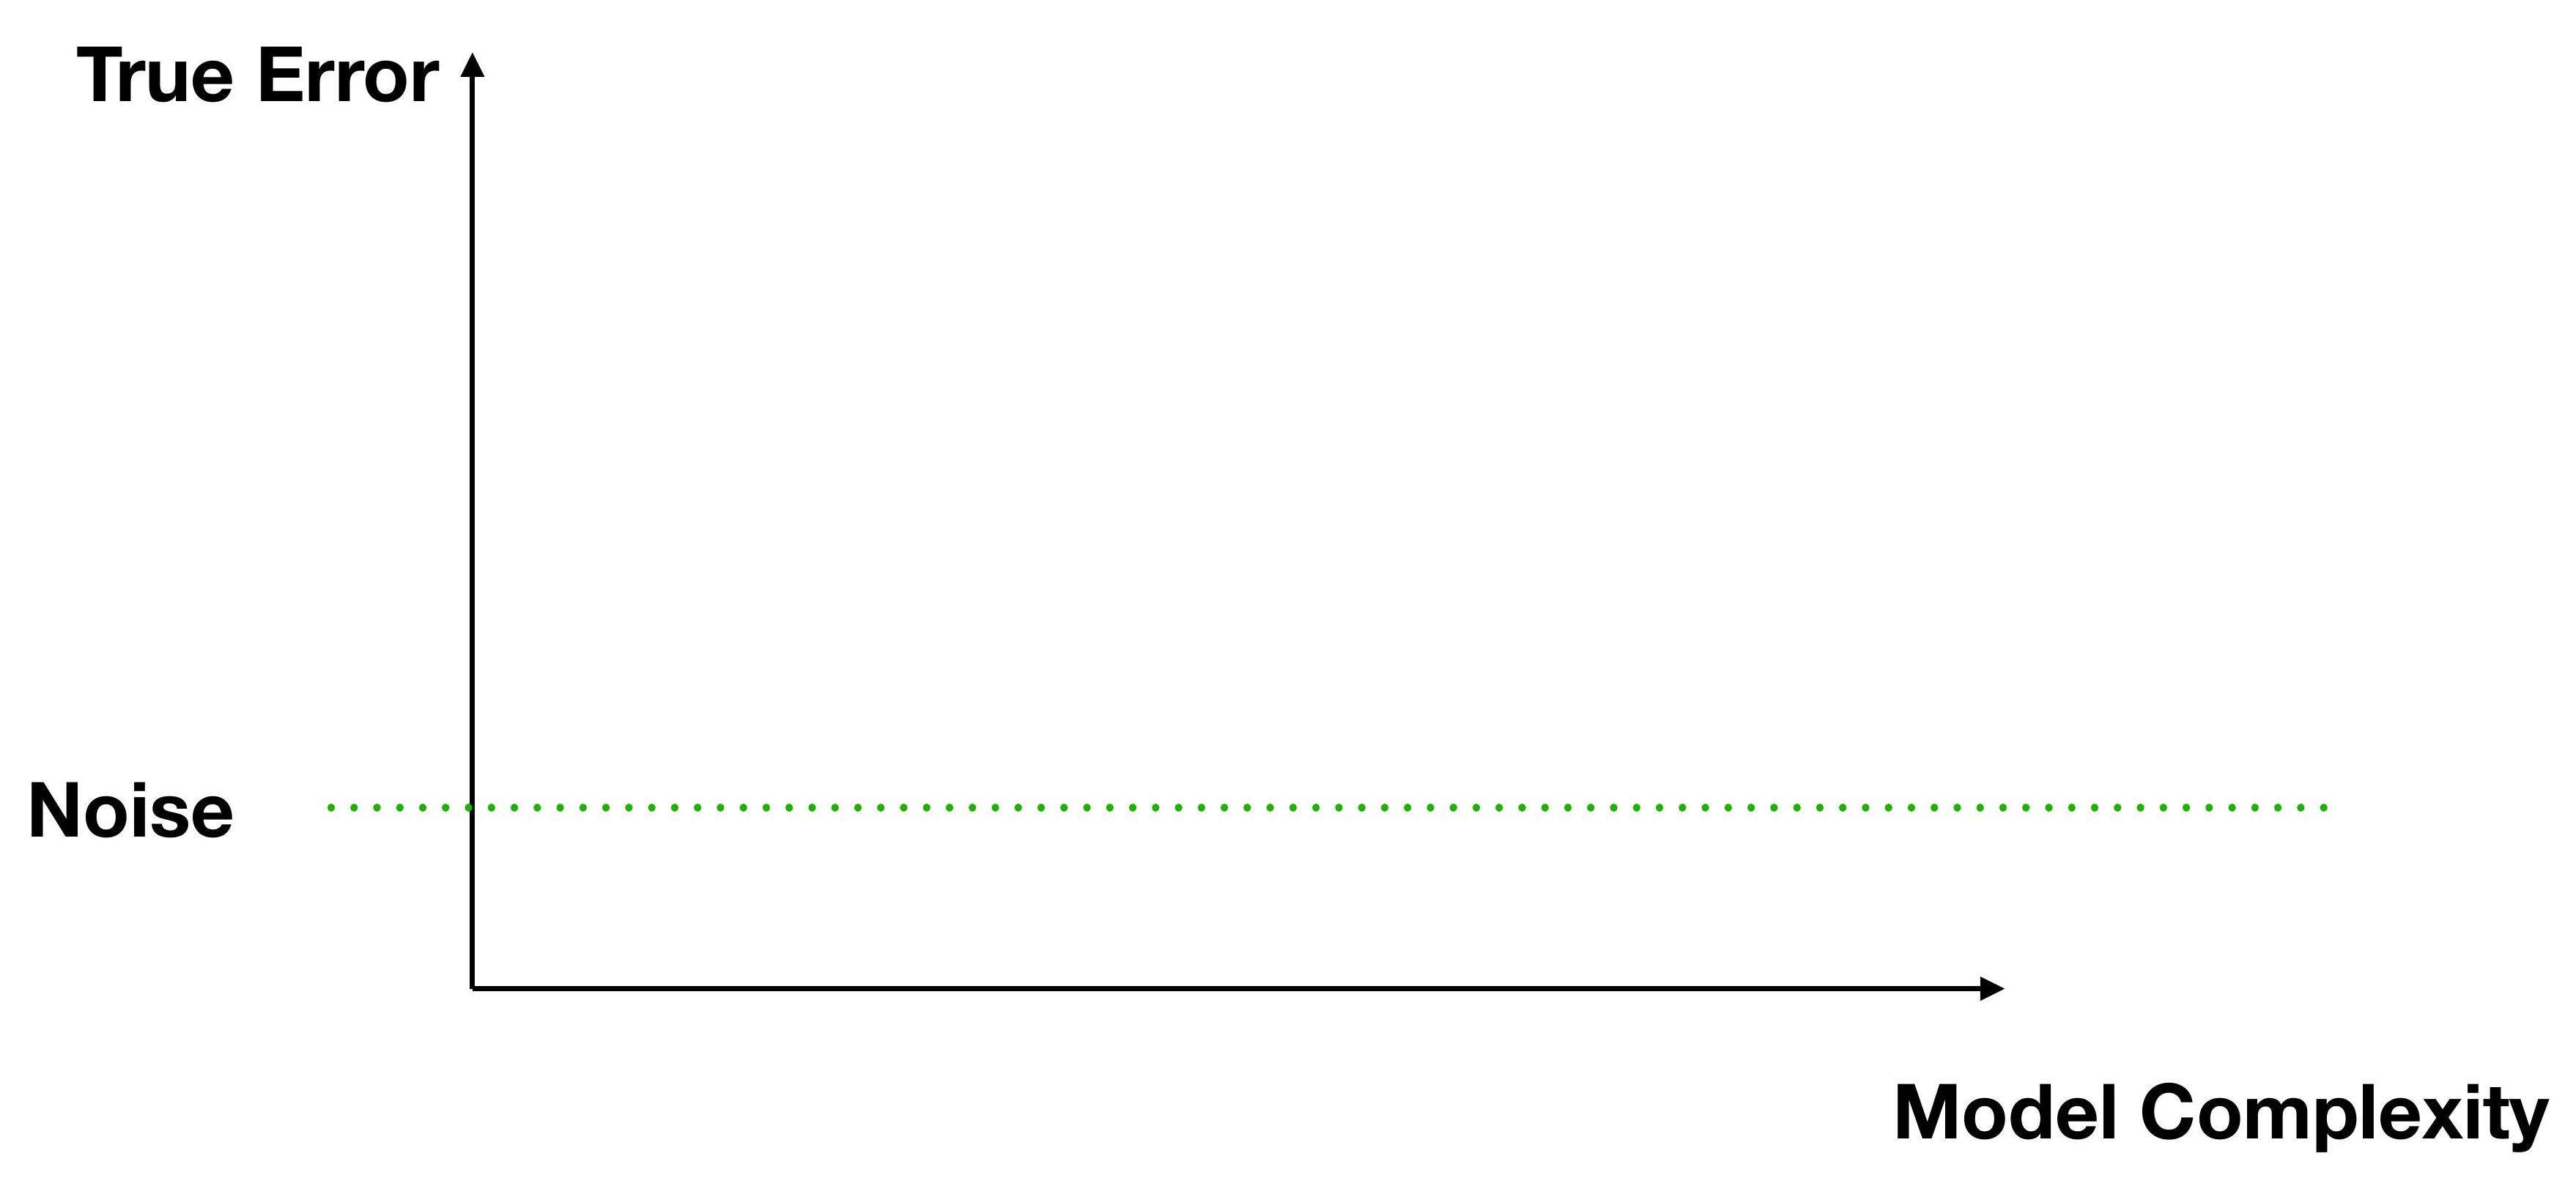
\includegraphics[max width=\textwidth]{2023_12_30_442f876157646883c2c9g-22}
\end{center}

\begin{itemize}
  \item It is not possible to go below the noise level

  \item Even if we know the true model $f$, we still suffer from the noise: $L(f)=\mathbb{E}\left[\varepsilon^{2}\right]$

  \item It is not possible to predict the noise from the data since they are independent

\end{itemize}

\section*{Bias: $\left(f\left(x_{0}\right)-\mathbb{E}_{S \sim \mathscr{D}}\left[f_{S}\left(x_{0}\right)\right]\right)^{2}$}
\begin{center}
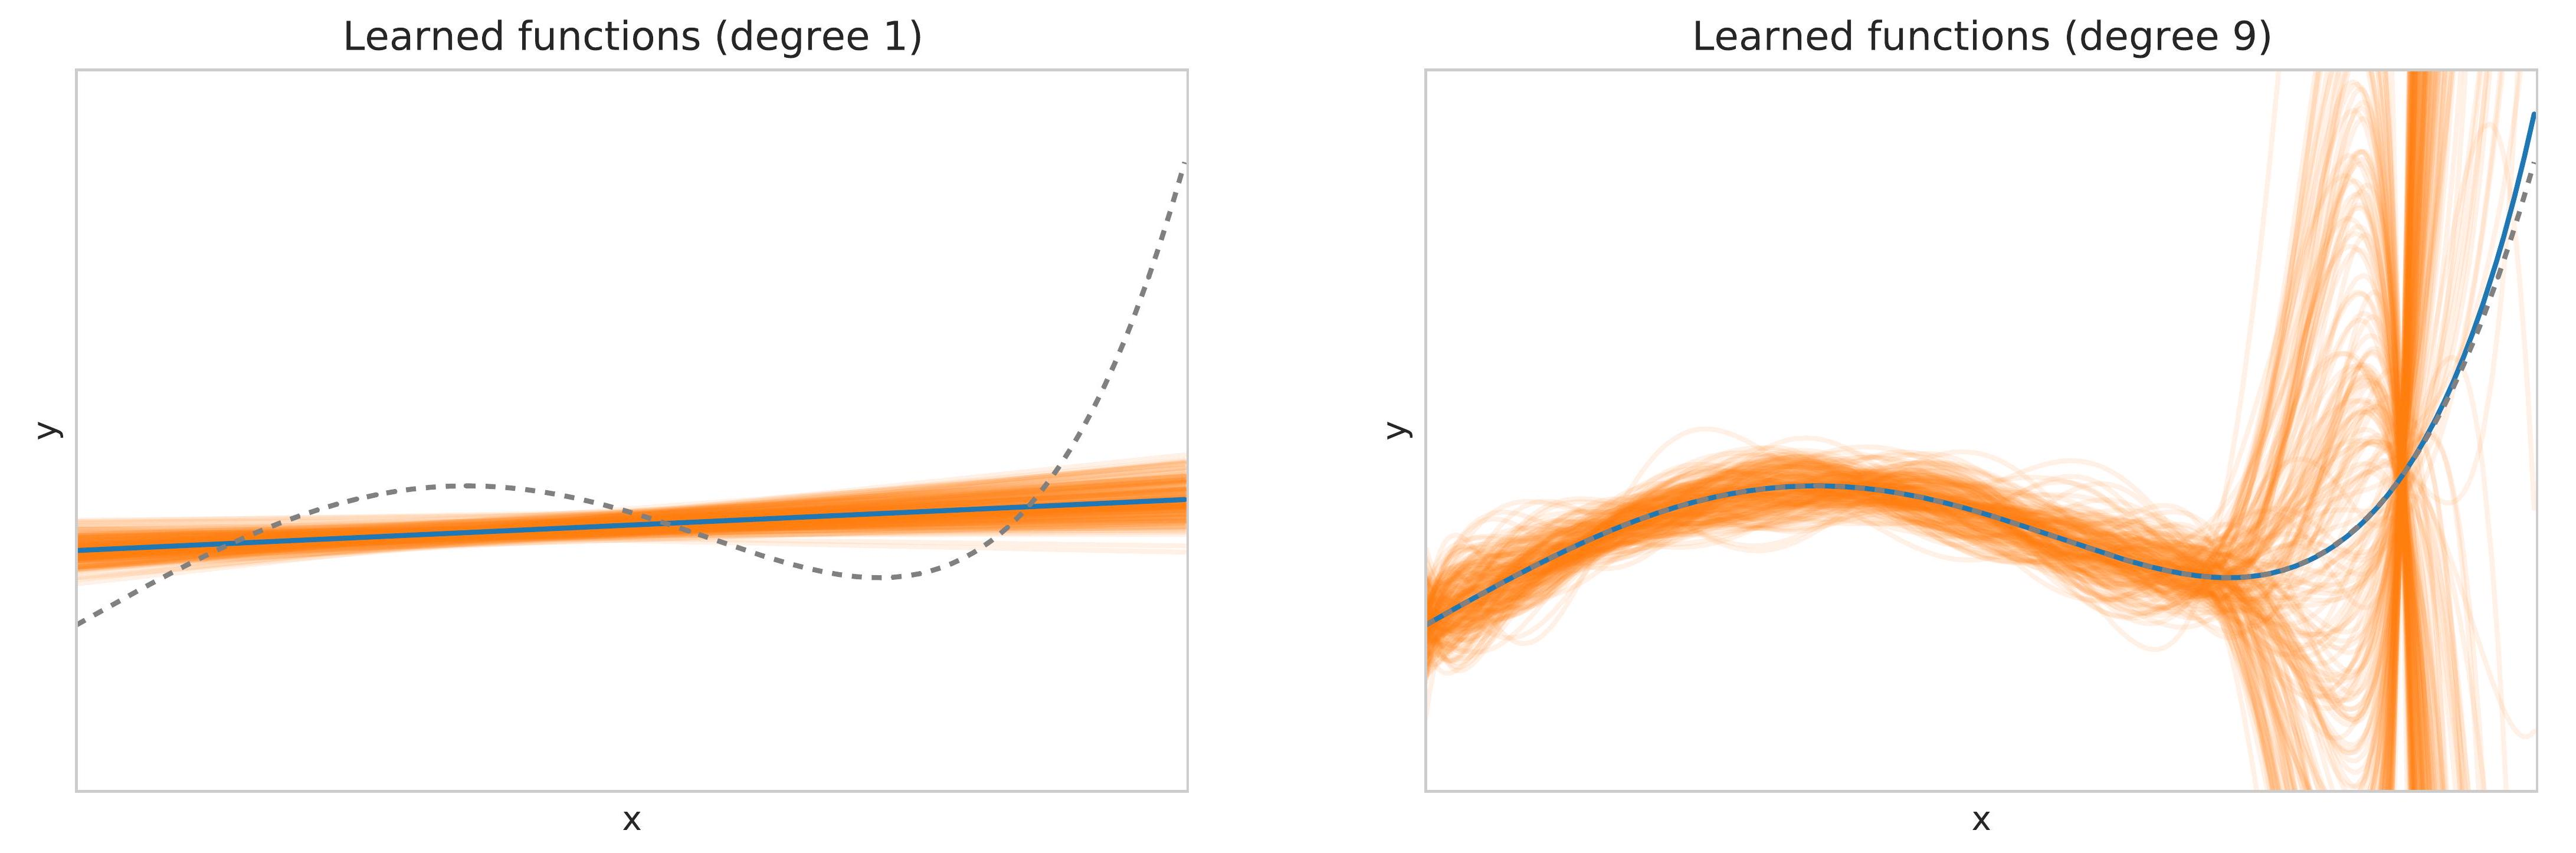
\includegraphics[max width=\textwidth]{2023_12_30_442f876157646883c2c9g-23}
\end{center}

\begin{itemize}
  \item Squared of the difference between the actual value $f\left(x_{0}\right)$ and the expected prediction

  \item It measures how far off in general the models' predictions are from the correct value

  \item If model complexity is low, bias is typically high

  \item If model complexity is high, bias Is typically low

\end{itemize}

\section*{Bias: $\left(f\left(x_{0}\right)-\mathbb{E}_{S \sim \mathscr{D}}\left[f_{S}\left(x_{0}\right)\right]\right)^{2}$}
\begin{center}
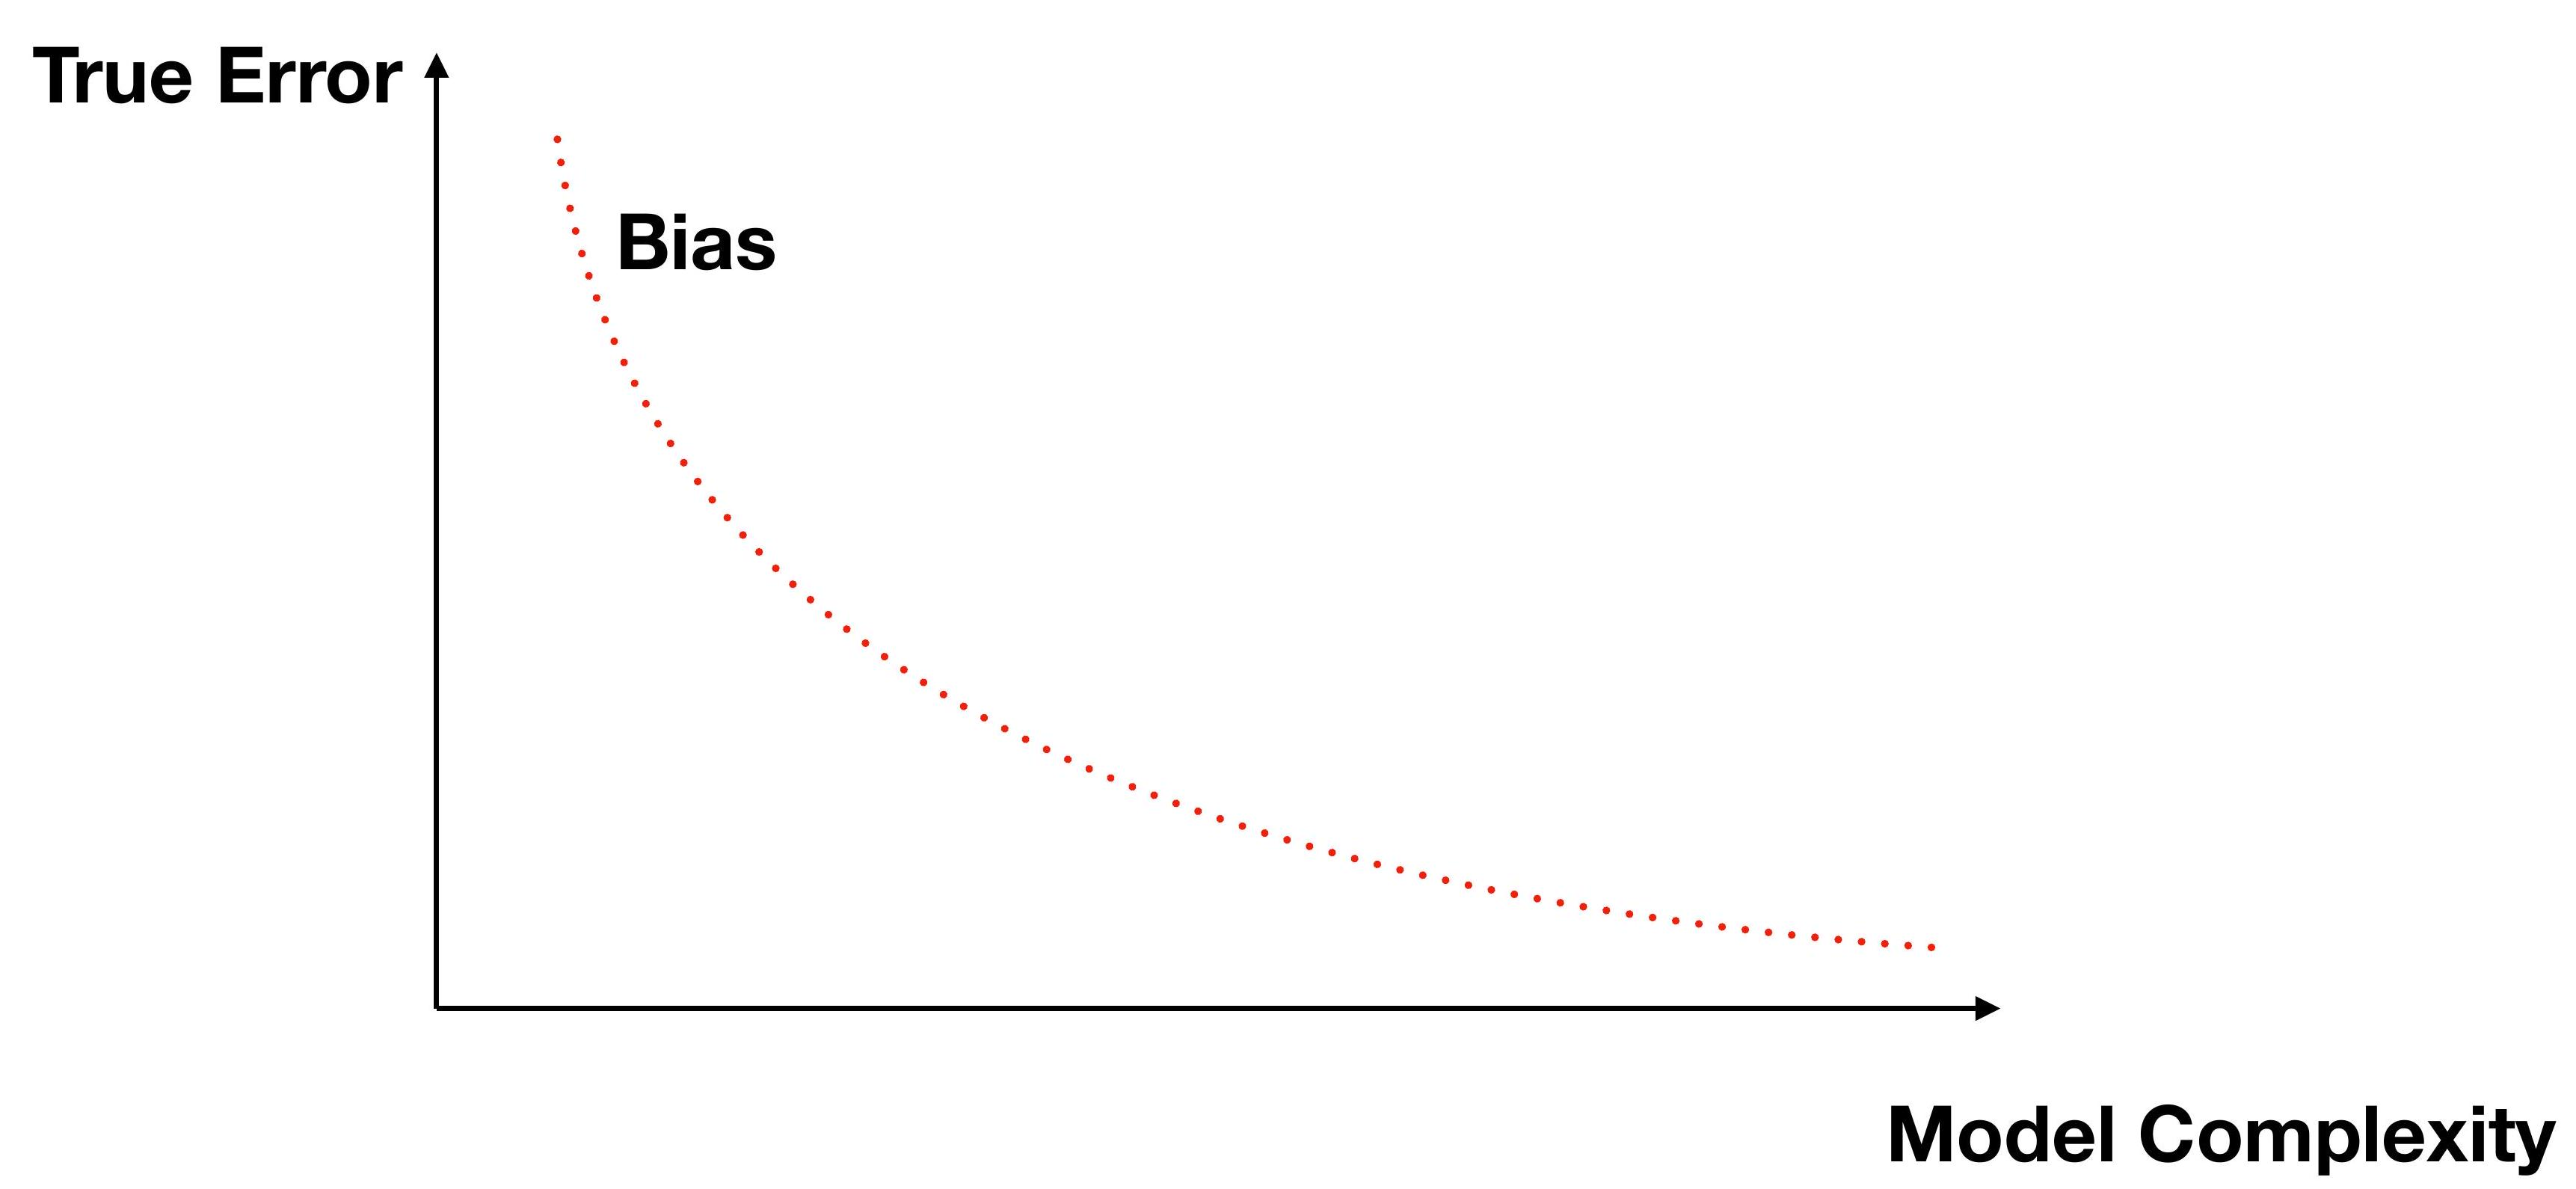
\includegraphics[max width=\textwidth]{2023_12_30_442f876157646883c2c9g-24}
\end{center}

\begin{itemize}
  \item Squared of the difference between the actual value $f\left(x_{0}\right)$ and the expected prediction

  \item It measures how far off in general the models' predictions are from the correct value

  \item If model complexity is low, bias is typically high

  \item If model complexity is high, bias is typically low

\end{itemize}

\section*{Variance: $\mathbb{E}_{S \sim \mathscr{D}}\left[\left(f_{S}\left(x_{0}\right)-\mathbb{E}_{S \sim \mathscr{D}}\left[f_{S}\left(x_{0}\right)\right]\right)^{2}\right]$}
\begin{center}
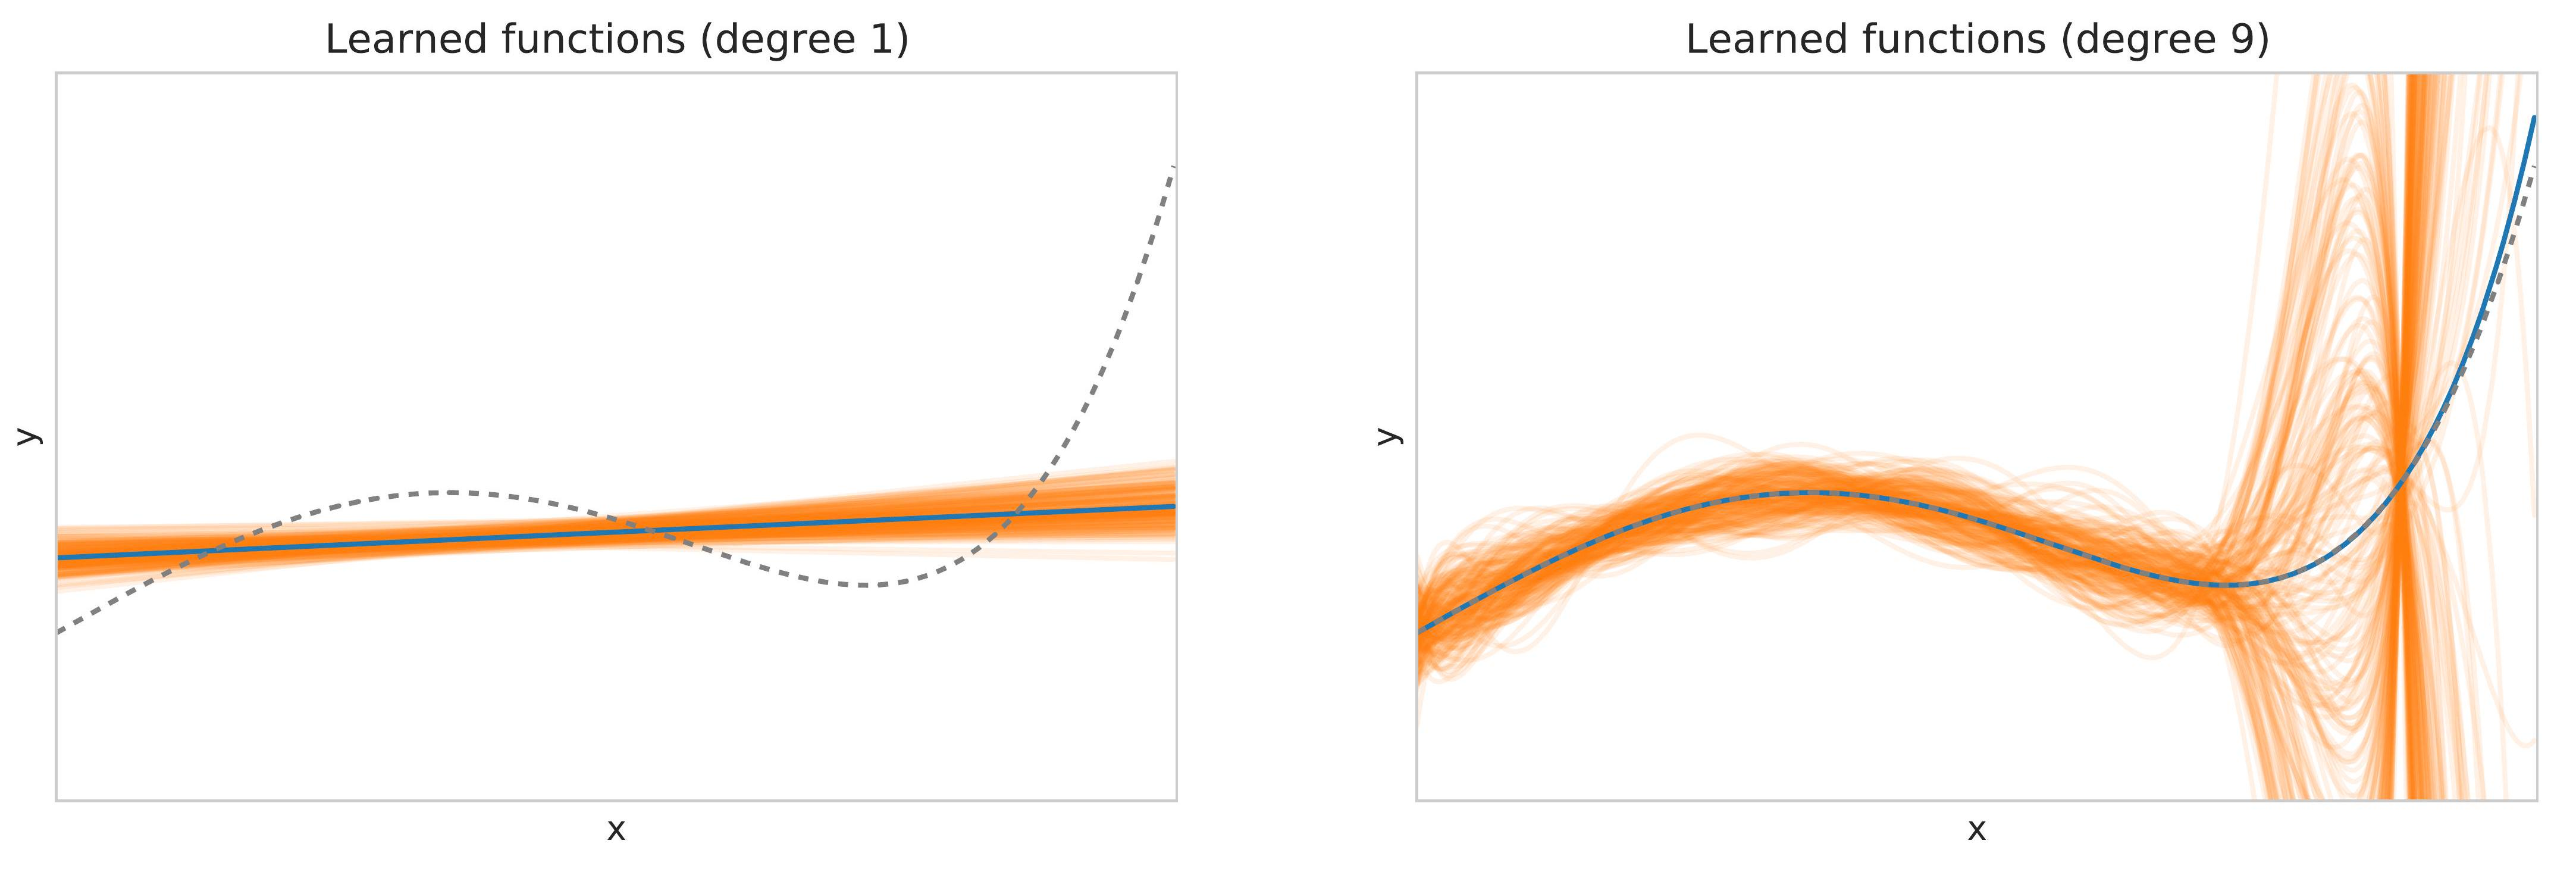
\includegraphics[max width=\textwidth]{2023_12_30_442f876157646883c2c9g-25}
\end{center}

\begin{itemize}
  \item Variance of the prediction function
  \item It measures the variability of predictions at a given point across different training set realizations
  \item If we consider complex models, small variations in the training set can lead to significant changes in the predictions
\end{itemize}

\section*{Variance: $\mathbb{E}_{S \sim \mathscr{D}}\left[\left(f_{S}\left(x_{0}\right)-\mathbb{E}_{S \sim D}\left[f_{S}\left(x_{0}\right)\right]\right)^{2}\right]$}
\begin{center}
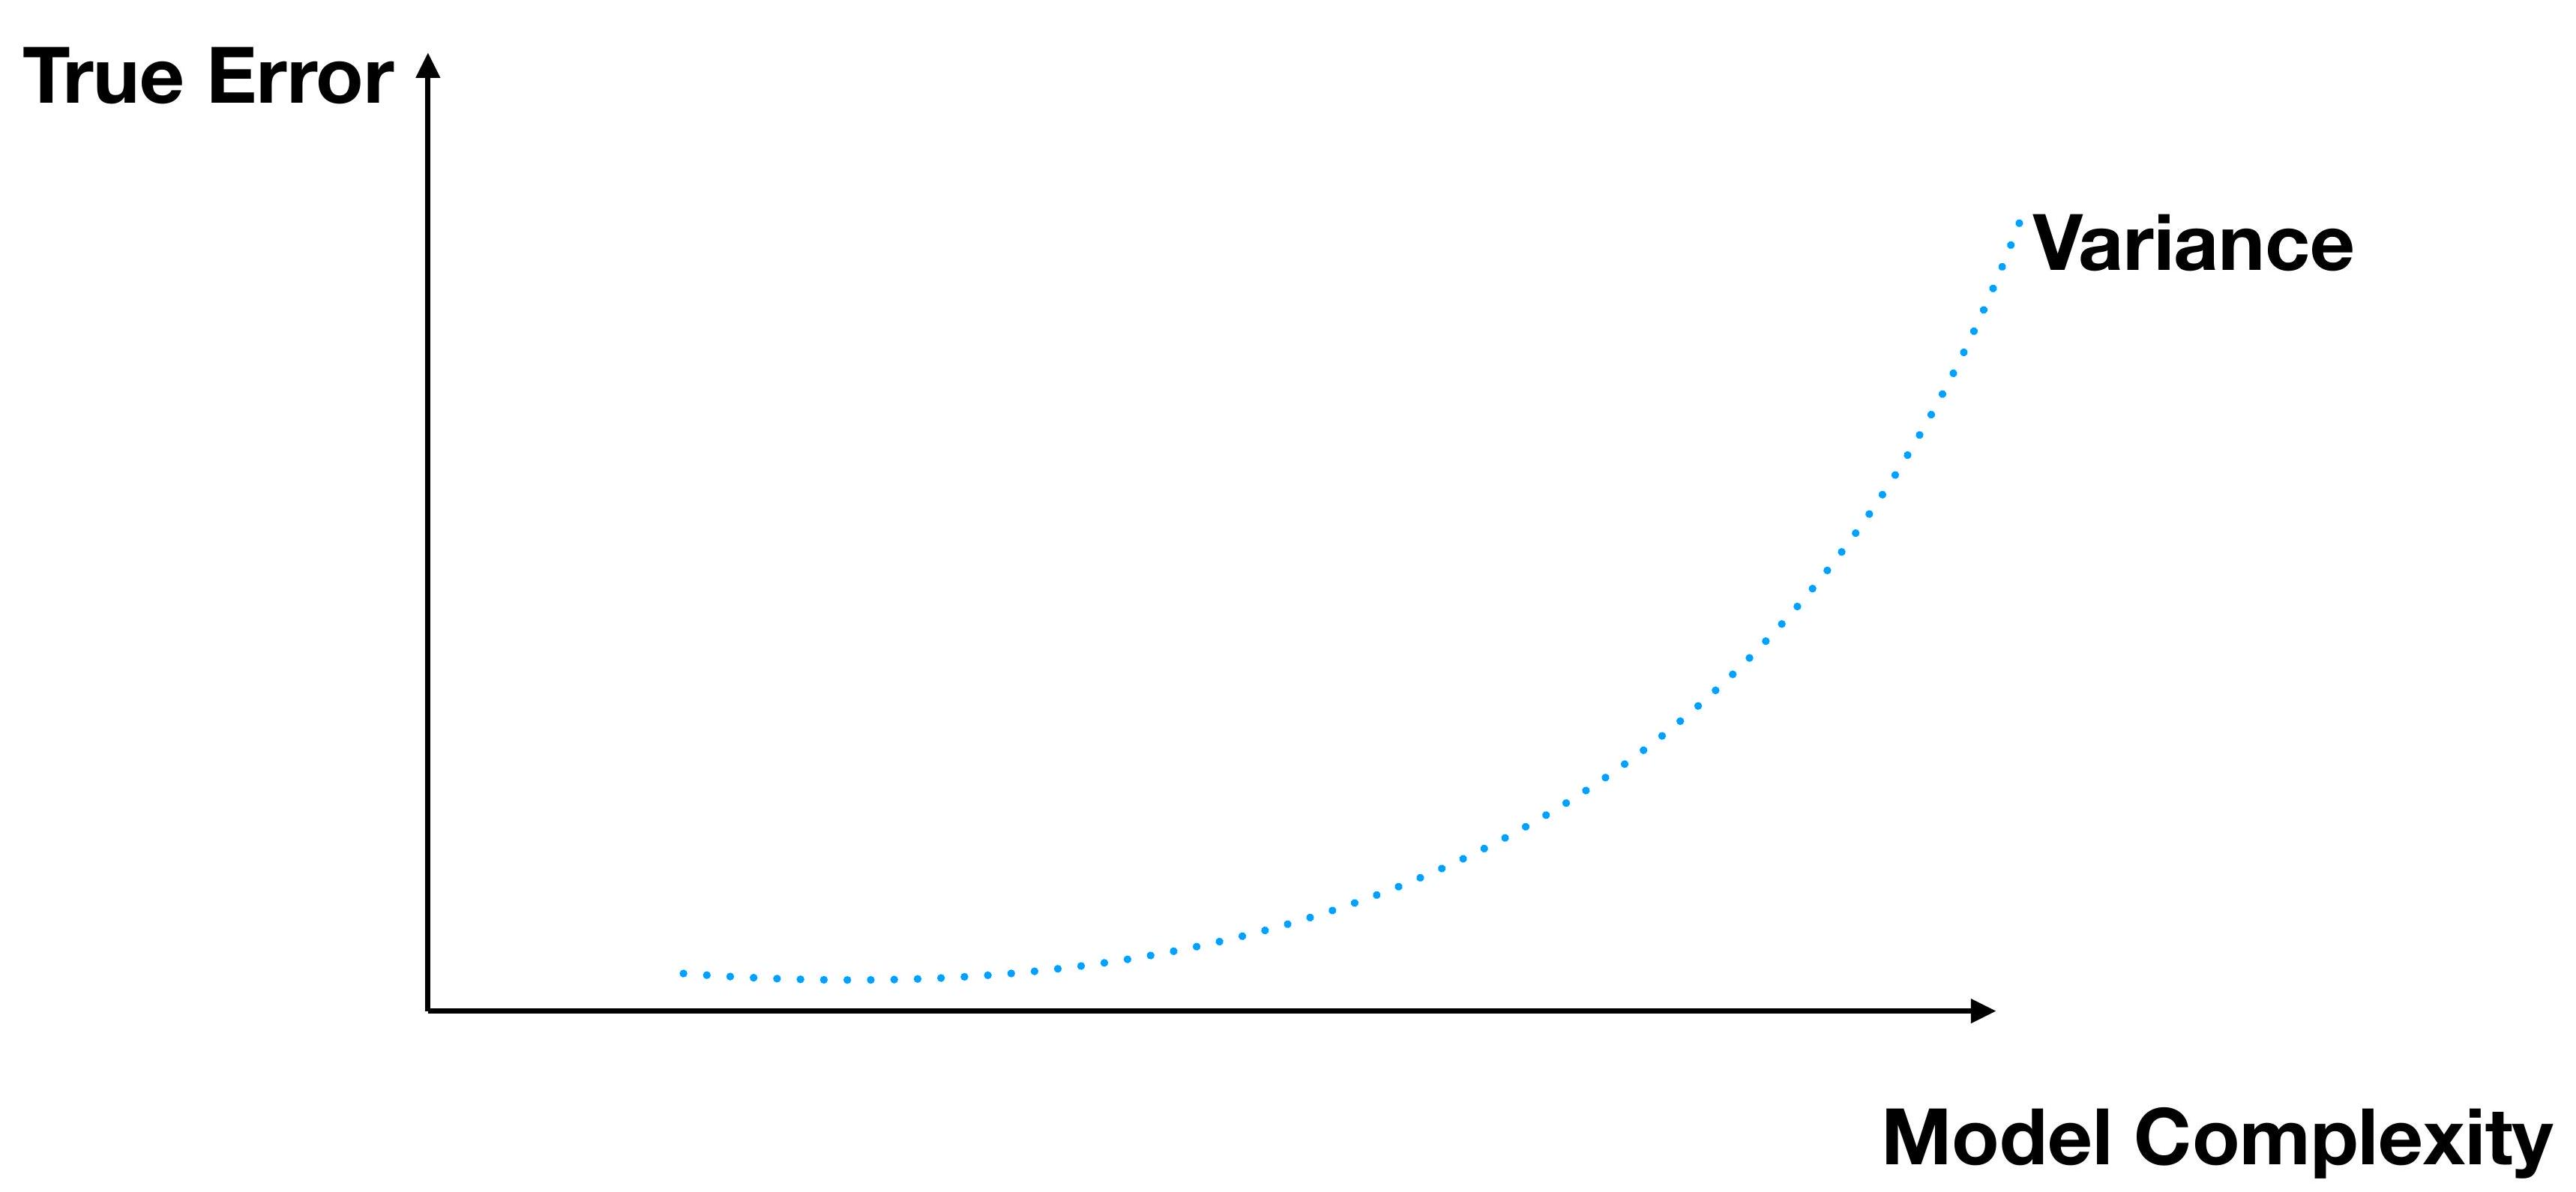
\includegraphics[max width=\textwidth]{2023_12_30_442f876157646883c2c9g-26}
\end{center}

\begin{itemize}
  \item Variance of the prediction function
  \item It measures the variability of predictions at a given point across different training set realizations
  \item If we consider complex models, small variations in the training set can lead to significant changes in the predictions
\end{itemize}

\section*{Bias Variance tradeoff and U-shape curve}
\begin{center}
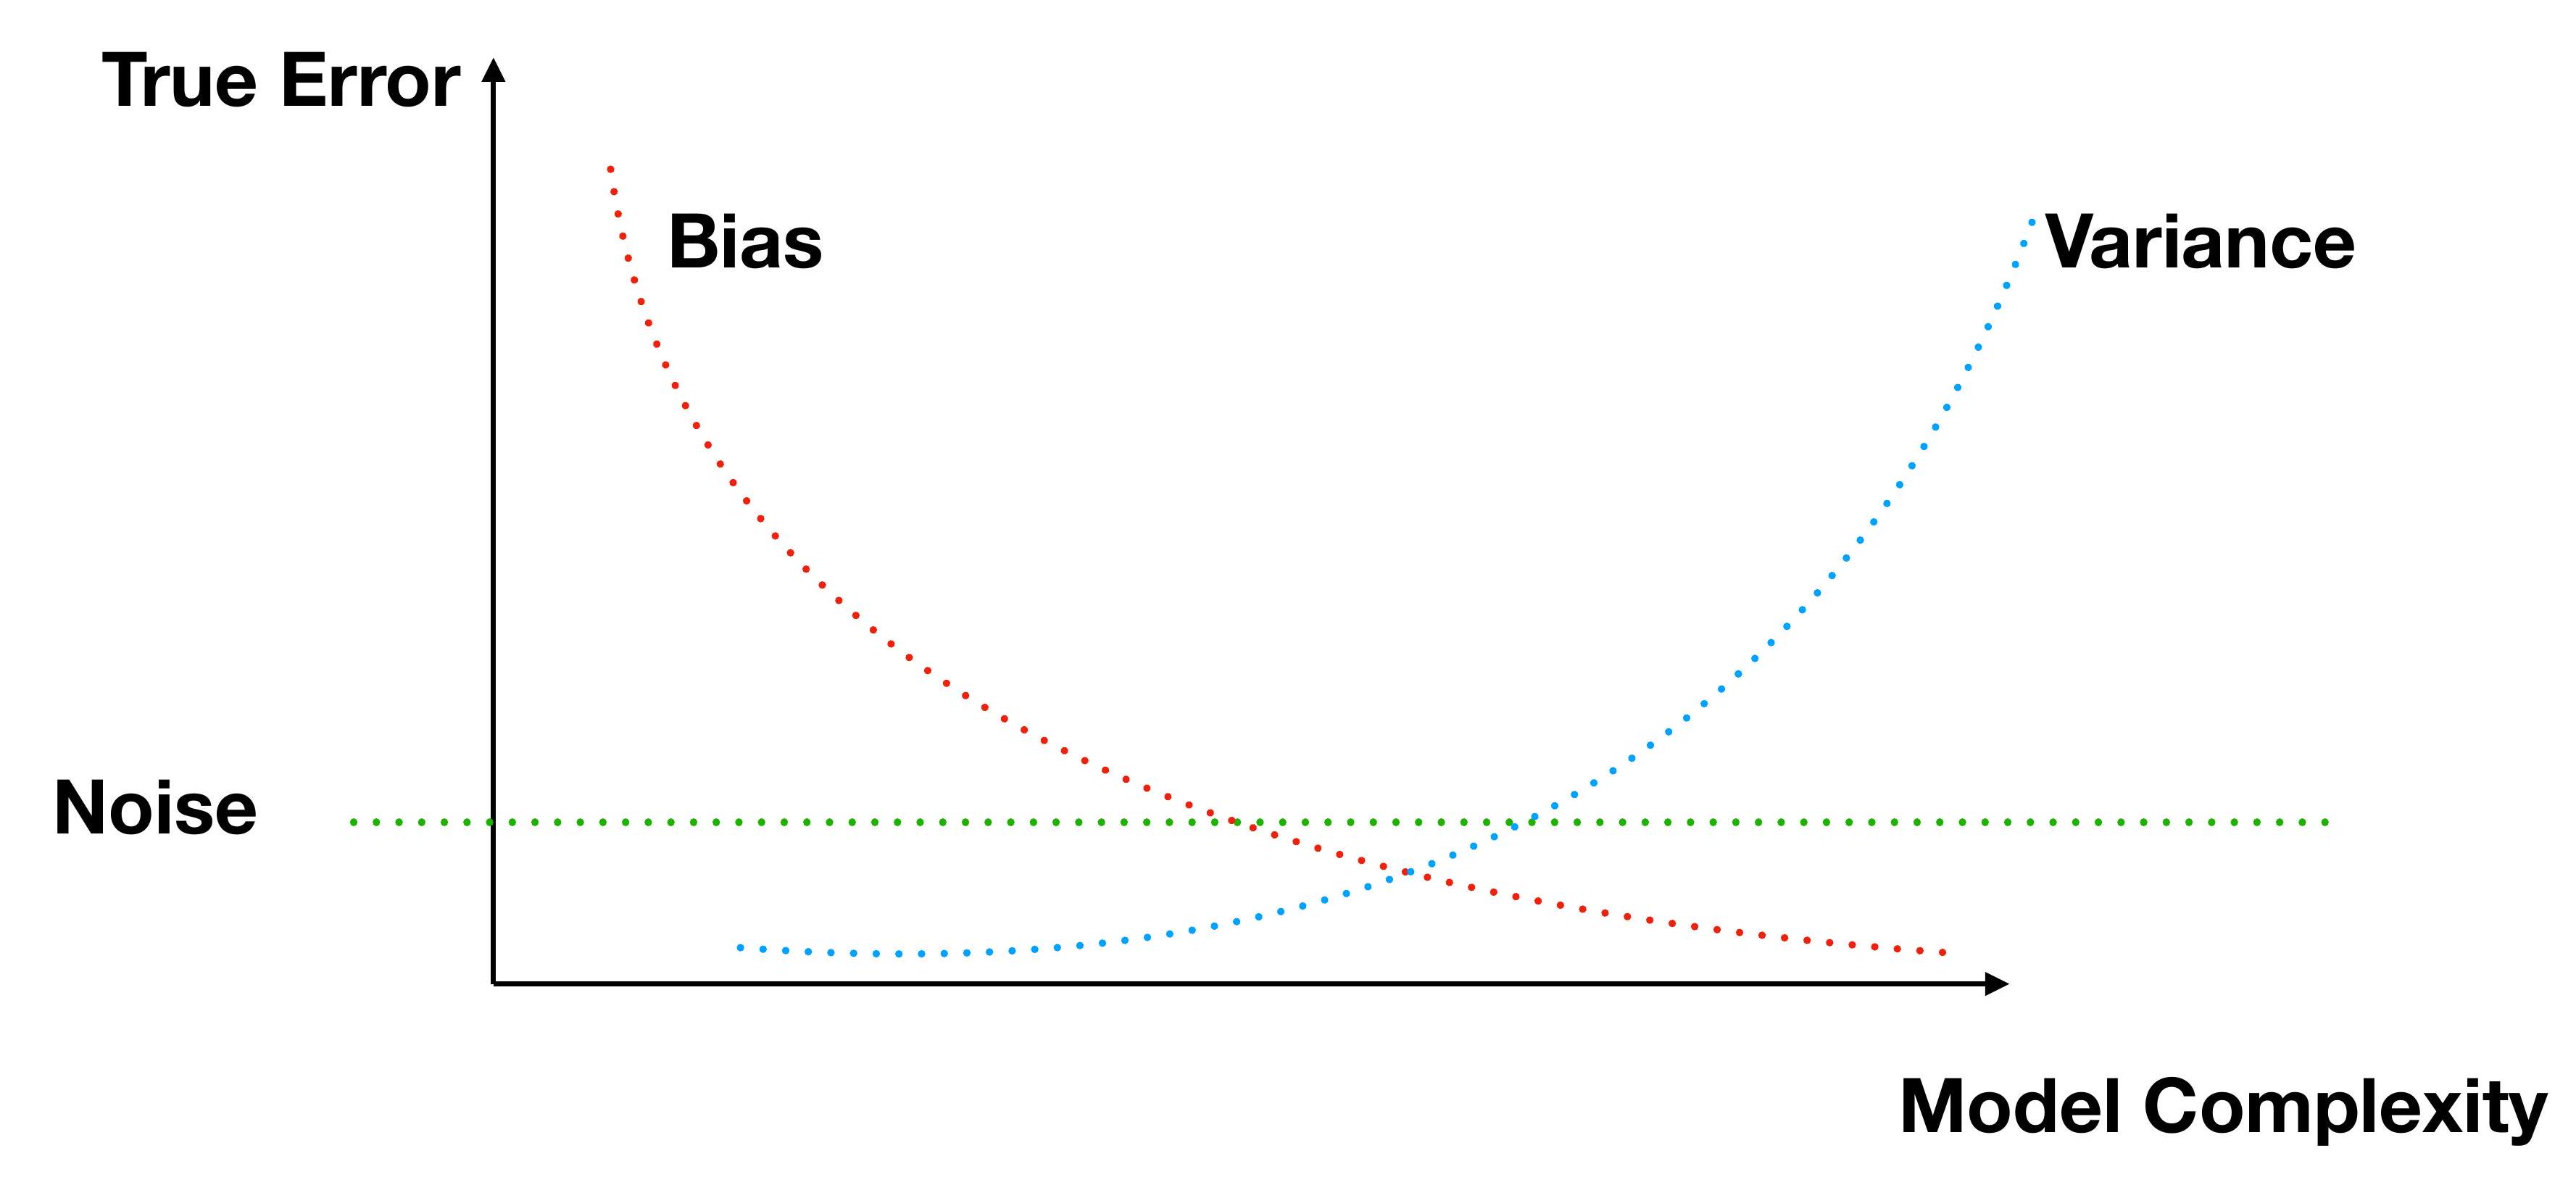
\includegraphics[max width=\textwidth]{2023_12_30_442f876157646883c2c9g-27}
\end{center}

\begin{itemize}
  \item If model complexity is too low, approximation will be poor (underfitting)

  \item If model complexity is too high, it may cause issues with variance (overfitting)

\end{itemize}

$\Rightarrow$ This phenomenon is known as the bias-variance tradeoff

\section*{Challenge: Identify a method that ensures both low variance and low bias}
\section*{Conclusion}
Low Variance

Low Bias

\begin{center}

\includegraphics[max width=\textwidth]{2023_12_30_442f876157646883c2c9g-29(1)}
\end{center}

High Bias

\begin{center}
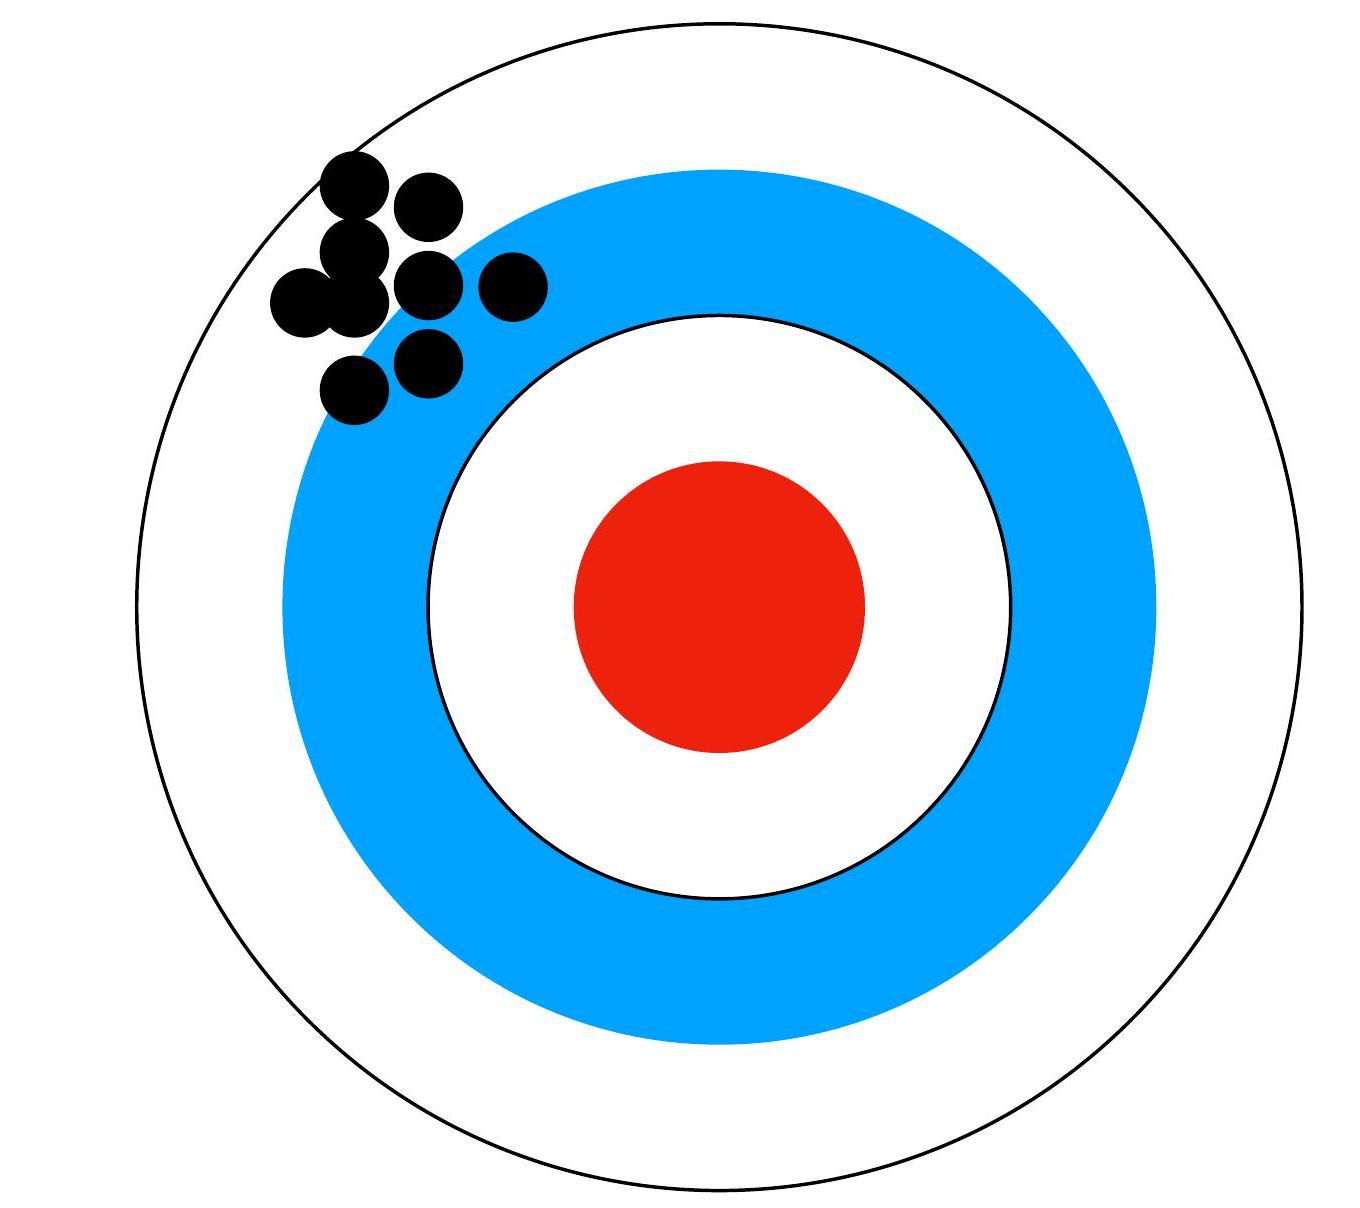
\includegraphics[max width=\textwidth]{2023_12_30_442f876157646883c2c9g-29}
\end{center}

High Variance
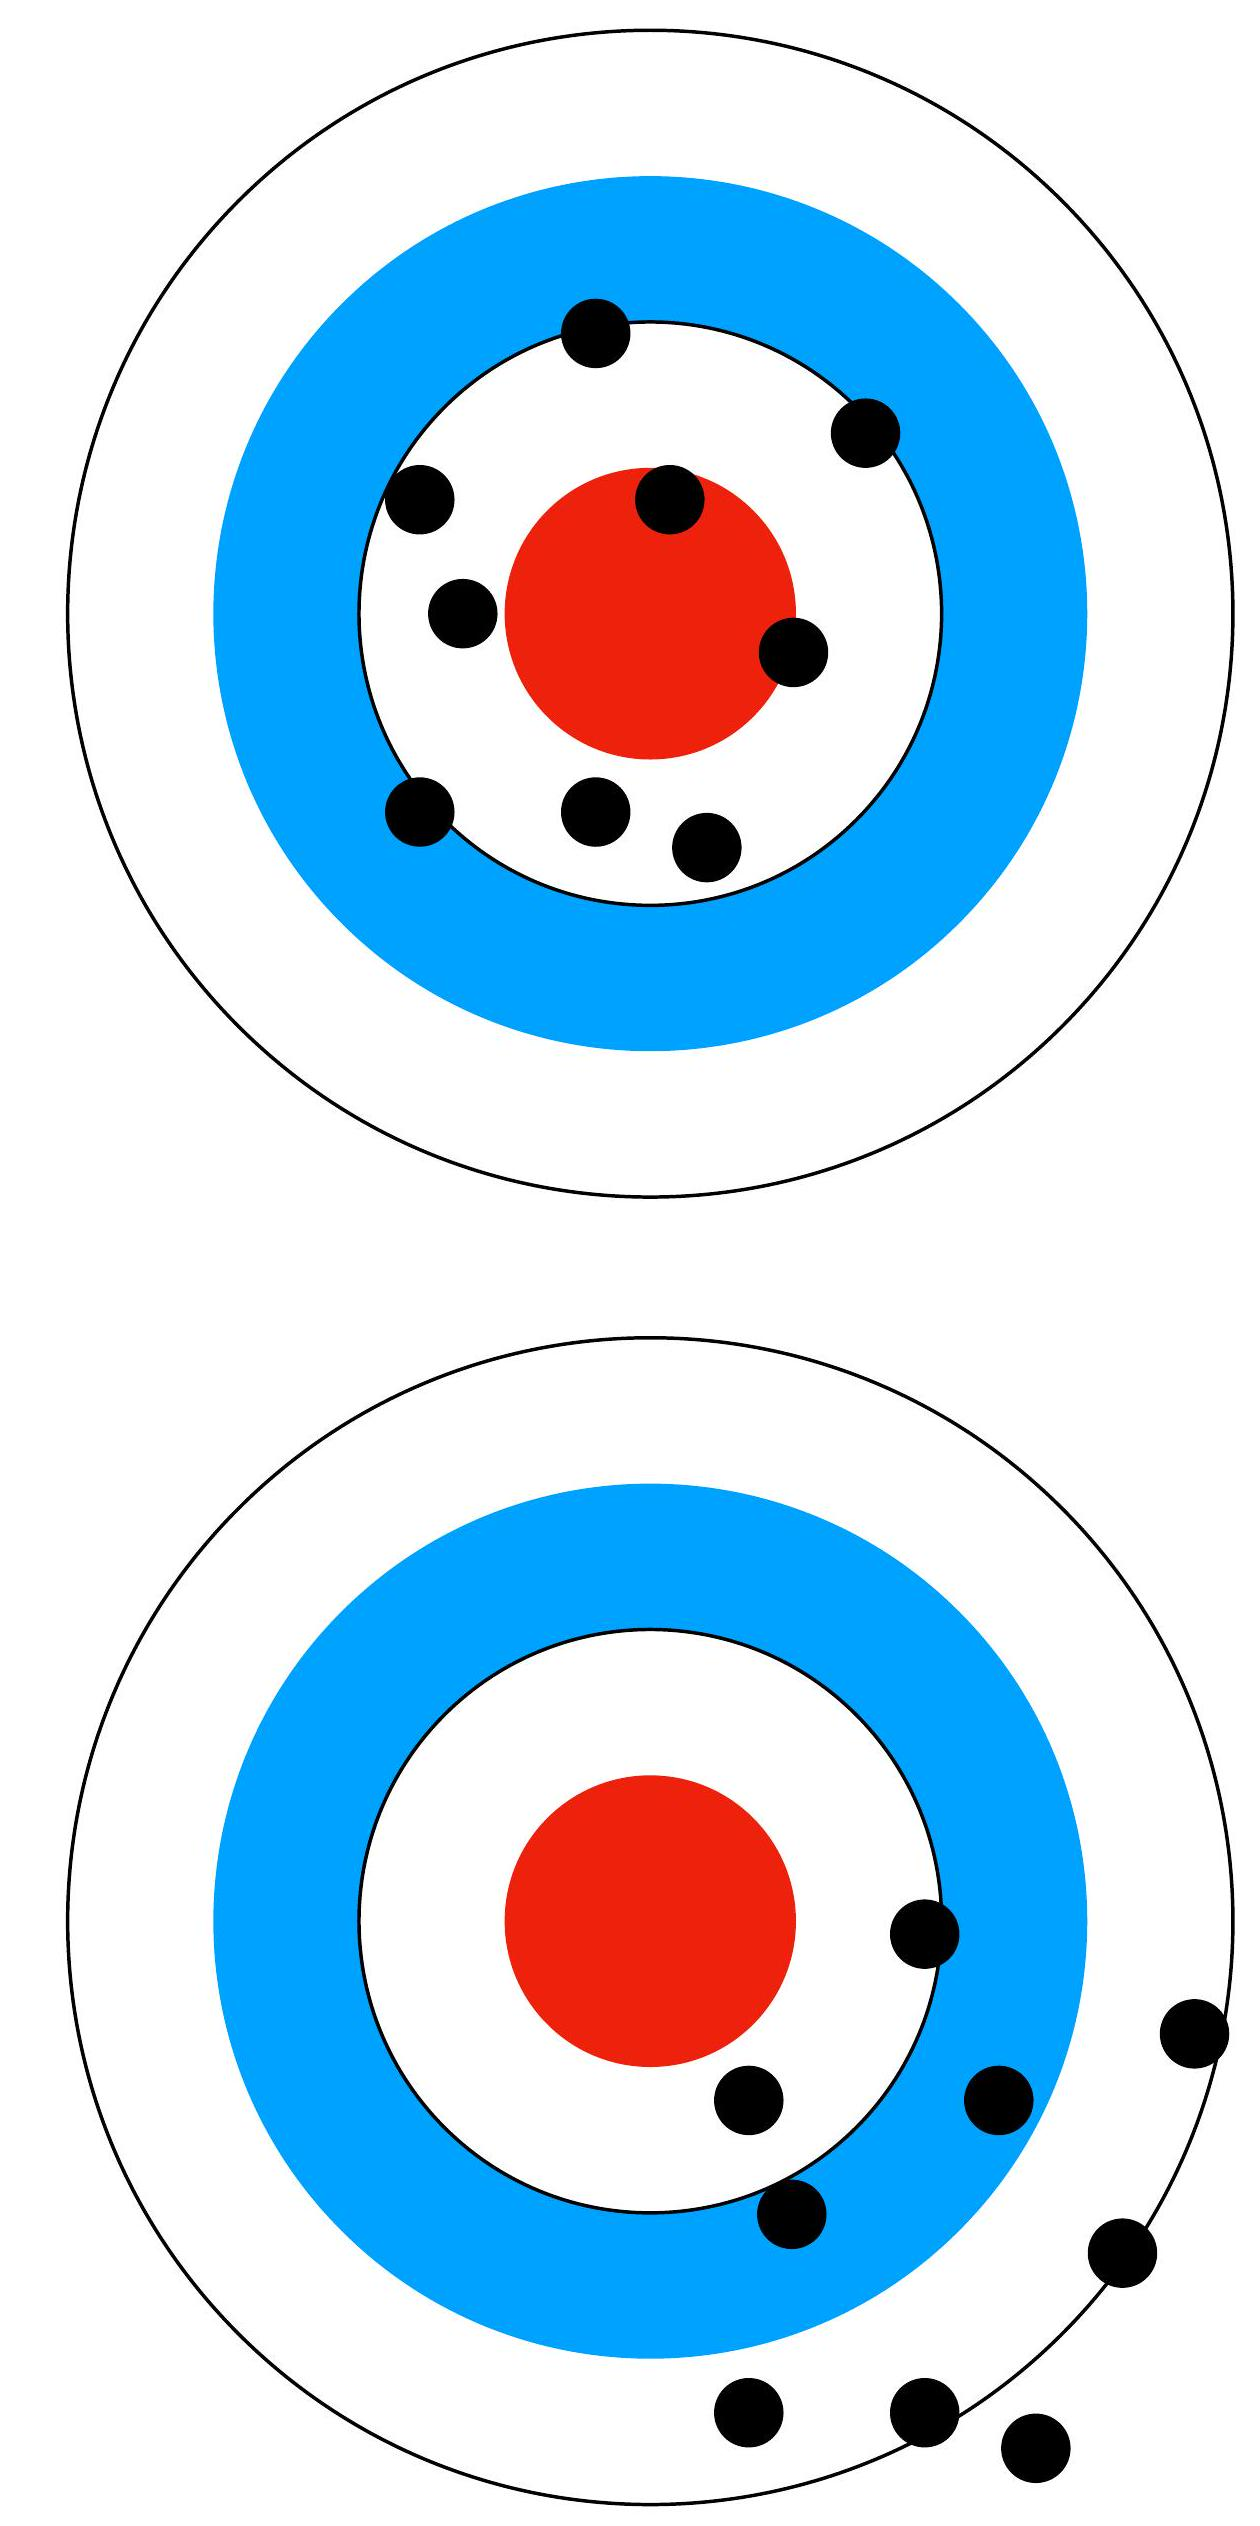
\includegraphics[max width=\textwidth, center]{2023_12_30_442f876157646883c2c9g-29(2)}

\section*{But this depends on the algorithm!}
\section*{Double descent curve}
\begin{center}
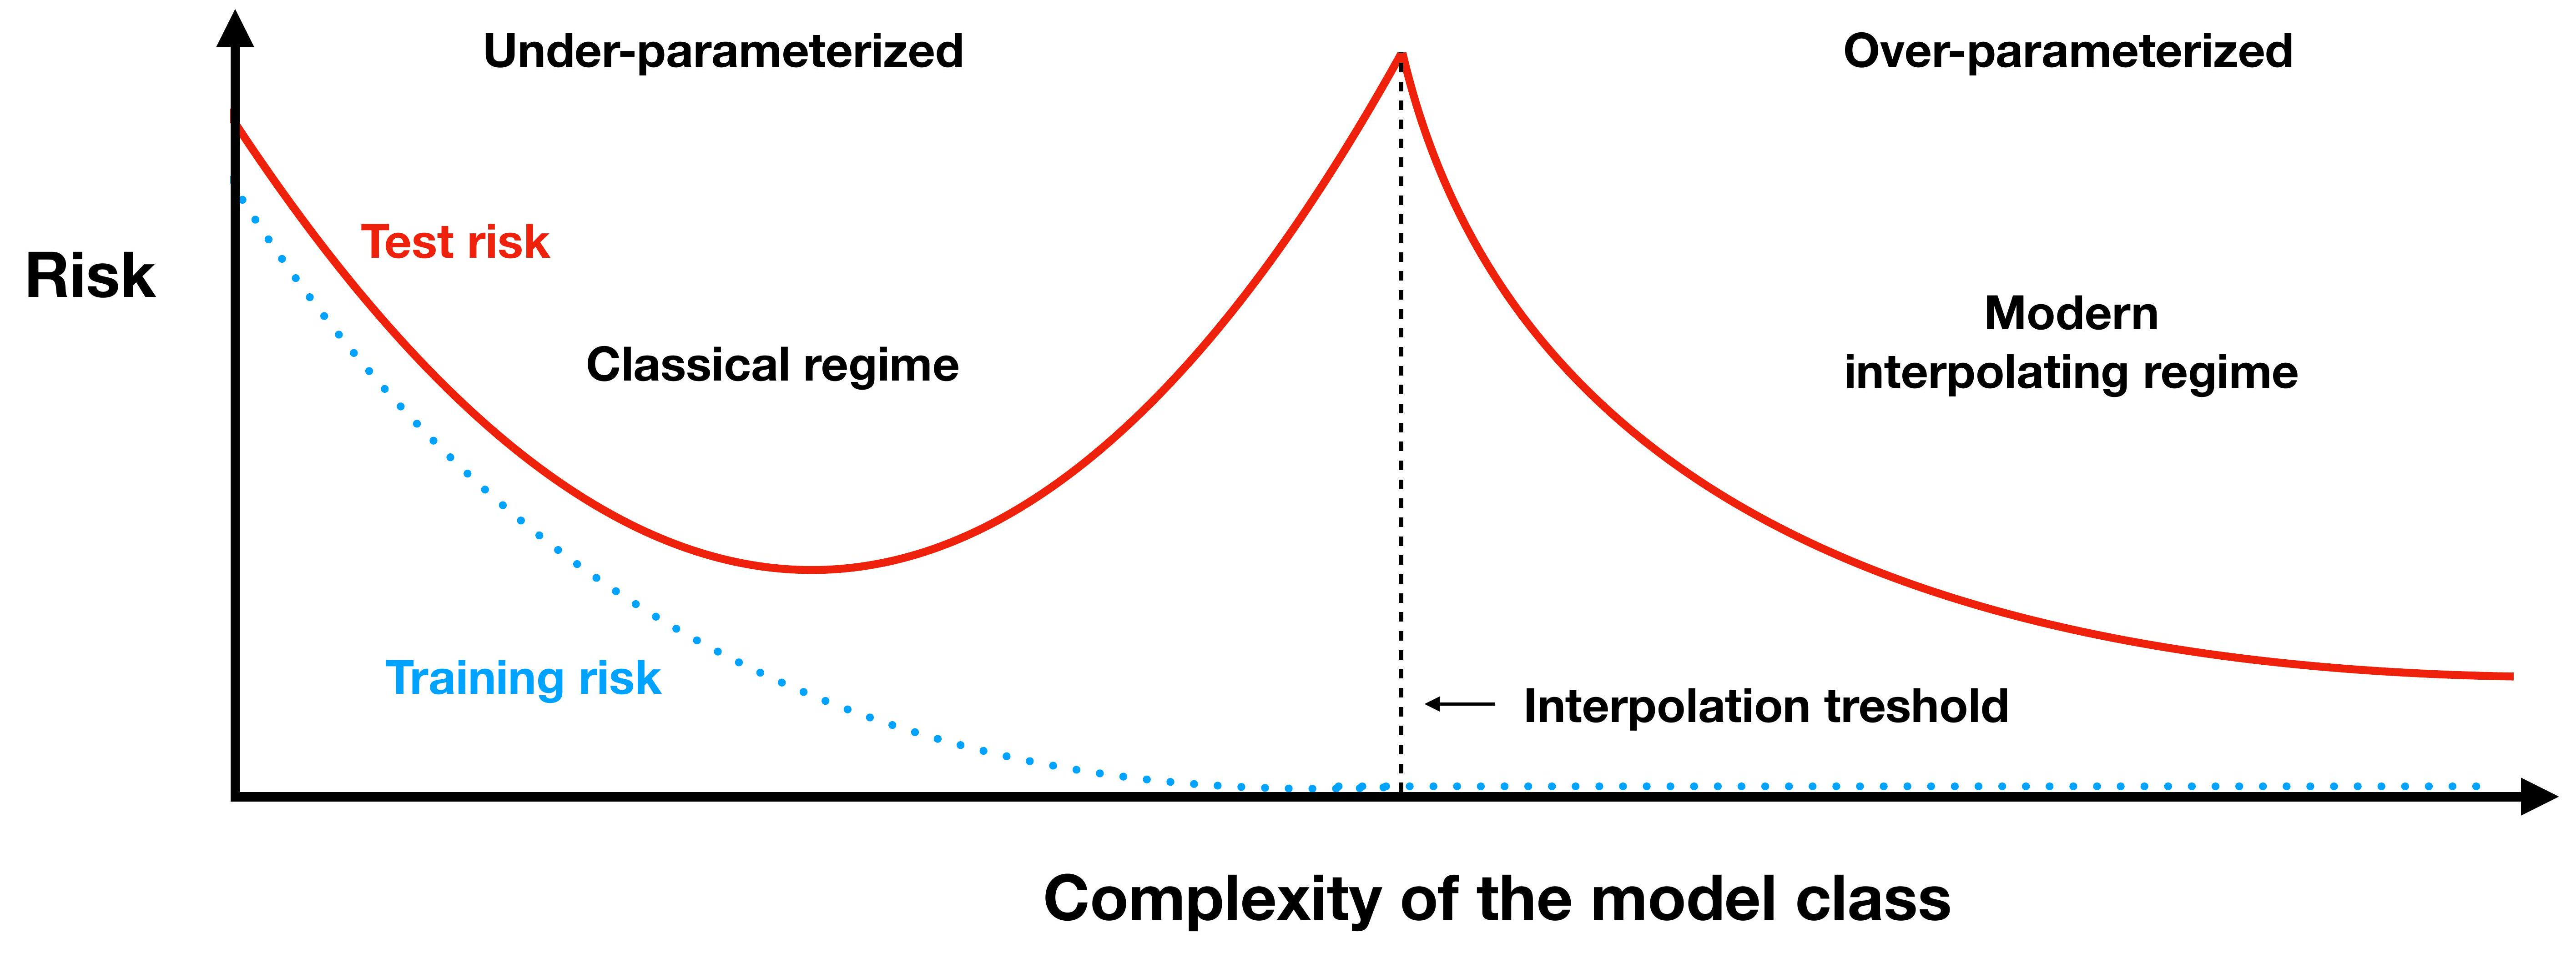
\includegraphics[max width=\textwidth]{2023_12_30_442f876157646883c2c9g-31}
\end{center}

Reconciling modern machine-learning practice and the classical bias-variance trade-off Mikhail Belkin, Daniel Hsu, Siyuan Ma, and Soumik Mandal, PNAS, 2019


\end{document}